% Created 2018-12-27 Thu 19:30
% Intended LaTeX compiler: xelatex
\documentclass[12pt,a4paper]{article}
\usepackage{graphicx}
\usepackage{grffile}
\usepackage{longtable}
\usepackage{wrapfig}
\usepackage{rotating}
\usepackage[normalem]{ulem}
\usepackage{amsmath}
\usepackage{textcomp}
\usepackage{amssymb}
\usepackage{capt-of}
\usepackage{hyperref}
\usepackage{fontspec}
\usepackage{xeCJK}
\usepackage{times}
\usepackage{booktabs}
\usepackage[table]{xcolor}
\usepackage{colortbl}
\usepackage{siunitx}

\setCJKmainfont[BoldFont={標楷體}]{標楷體}
\setmainfont{TeX Gyre Termes}
\renewcommand\tablename{表}
\renewcommand\figurename{圖}
\renewcommand{\contentsname}{目次}
\renewcommand{\listtablename}{表次}

\bibliographystyle{plain}
\bibliography{../references}
\parindent=25pt
\definecolor{contiYellow}{RGB}{255,165,0}

\makeatletter
\renewcommand\tableofcontents{%
  \section*{\huge\contentsname
    \@mkboth{%
      \MakeUppercase\contentsname}{\MakeUppercase\contentsname}}
  \setcounter{page}{1}
  \pagenumbering{Roman}
  \@starttoc{toc}%
}
\renewcommand\listoffigures{%
  \section*{\huge\listfigurename
    \@mkboth{%
      \MakeUppercase\listfigurename}{\MakeUppercase\listfigurename}}
  \@starttoc{lof}%
}
\renewcommand\listoftables{%
  \section*{\huge\listtablename
    \@mkboth{%
      \MakeUppercase\listtablename}{\MakeUppercase\listtablename}}
  \@starttoc{lot}%
  \newpage
  \pagenumbering{arabic}
}
\makeatother

\usepackage{amssymb}
\usepackage{xpatch}
\makeatletter
\xpatchcmd{\@maketitle}
          {\@title}
          {\thispagestyle{empty}
            \large 科發基金管理會補助計畫成果報告 \\
            \vskip 1em%
          社會與科技政策溝通平台計畫 \\
          \@title
          }
          {}{}

\xpatchcmd{\@maketitle}
          {\@date}
          {\large
            \vskip 10em
            %% \@date \\
            \begin{flushleft}
              \normalsize
              $\blacksquare$ 本計畫除繳交成果報告外,另含下列出國報告,共\underline{\ \ \ \ \ \ }份:\\
              $\square$ 執行國際合作與移地研究心得報告\\
              $\square$ 出席國際學術會議心得報告\\

              \vskip 1.5em

              報告處理方式:
              \begin{enumerate}
                \itemsep -12pt
              \item 公開方式:\\
                $\square$ 非列管計畫亦不具下列情形,立即公開查詢\\
                $\square$ 涉及專利或其他智慧財產權,□一年□二年後可公開查詢\\
              \item 「本研究」是否已有嚴重損及公共利益之發現:$\square$否 $\square$是\\
              \item 「本報告」是否建議提供政府單位施政參考 $\square$否 $\square$是,\underline{\ \ \ \ }(請列舉提供之單位;本會不經審議,依勾選逕予轉送)\\
              \end{enumerate}
              \vskip 2em
              委託單位:行政院科技會報辦公室\\
              執行單位:計畫分項執行團隊名稱\\
            \end{flushleft}
            \vskip 2em
            \begin{center}
              中\hspace{12pt}華\hspace{12pt}民\hspace{12pt}國\hspace{60pt}年\hspace{60pt}月\hspace{60pt}日
            \end{center}
            \newpage
          }
          {}{}
\makeatother

\author{陳信屹、簡韻真、黃凱蘭、黃宇新}
\date{\today}
\title{如何促進科技社群網路參與科技政策討論建議報告 - 以資訊科技社群為例 (草稿)}
\hypersetup{
 pdfauthor={陳信屹、簡韻真、黃凱蘭、黃宇新},
 pdftitle={如何促進科技社群網路參與科技政策討論建議報告 - 以資訊科技社群為例 (草稿)},
 pdfkeywords={},
 pdfsubject={},
 pdfcreator={Emacs 27.0.50 (Org mode 9.1.14)},
 pdflang={Zh-Tw}}
\begin{document}

\maketitle
\tableofcontents

\listoftables
\listoffigures
\section{中文摘要}
\label{sec:org2d99149}
本研究針對「數位原民」為主之網路科技社群,設計一套線上線下串接議題釐清機制,以建立公民參與意願與公共討論品質,讓網路社群能自組織發起討論並且論述有足夠議事資本可影響科技政策。本研究以資訊科技社群為例,以服務藍圖、顧客旅程等服務設計方法,拆解公民參與階段,並針對「前期議題設定」、「議題發酵」兩階段之溝通落差,以敏捷開發線上意見整理工具與線下議題小聚,研究發現透過問答、名詞定義、補充資料來源、界定利害關係人等原則做深度議題釐清達到與會者知識語彙對齊、提升論述品質,其中以線下實體參與建立參與意願與個人連結,線上數位記錄做網路擴散與延續討論,使線上線下串連達成網路社群低成本、高頻之自組織討論方式凝聚共識、釐清爭點。然本研究尚未達到網路效應,無法在特定議題上做到完善之回應建構評估之多方利害關係人參與討論。針對政府則建議(1)開放易搜尋與互相連結之資料補足民間與政府知識落差,(2)鼓勵社群討論與提供會議紀錄及會議參考資料,(3)加入社群討論。

\textbf{實踐社群}, \textbf{線上參與}, \textbf{issue mapping}, \textbf{論點圖}
\section{英文摘要}
\label{sec:org48ae2d7}
We develop an online-offline issue-mapping civic discussion process to empower cyber communities of practice to generate high quality discourse in order to influence technology policy in pre-evaluation stage. The civic participation process of digital natives in Taiwan is examined through service blueprint and customer journey map. Identifying the key communication gaps in agenda setting and issue discussion process, we develop an integrated process of an online annotation and concept mapping tool and offline issue-mapping meetups to include cyber communities to initiate responsive constructive evaluation process on social issues and policies. The offline meetups connect active participants and inspire further online discussion. The low entry barriar discussion generates high quality discussion based on questioning and  answering, term definition, supporting sources, and identifying stakeholders. By crowdsourcing micro activities constructing opinions and policies suggestion with above principles, cyber communities are able to identify key arguments on certain issues in serious discussion.

\textbf{community of practice}, \textbf{online participation}, \textbf{issue mapping}, \textbf{argument map}
\section{前言}
\label{sec:org5a6d993}
\texttt{需要修正讀起來的是否順暢}
「1970 年代後,公共政策學者開始修正鐵三角理論,認為實際的政策過程並非如鐵三角理論所描述的封閉,實則有許多公私組織參與其中」 \citep*{luo15_gong} ,台灣亦有學者以全民健保政策改革為例,針對「政策利害關係人」(William N. Dunn,1994)形成的網路關係進行研究,發現「當政策屬於規劃階段,不論就政策的資訊獲得、交換或是議題的資訊來源,均能形成由公、私與第三部門所組成的資訊網絡。政府部門不再被認為擁有獨占的專業知識,必須依賴私部門與第三部門提供政策資訊與諮詢,同時成為政策夥伴。」\citep{luo2005} ,但「由於顧主導向的政策研究,往往未能或是沒有興趣指認『沉默的輸家』」\citep*{chen11} ,一旦正式會議未處理政策弱勢的代表性議題,公眾只要沒有透過培力或動員來建構其代表性基礎,將在會議中缺乏議事資本,也導致決策缺乏草根性和正當性 \citep*{lo17}。

今日,數位原民 \citep*{prensky2001digital} 以社群為網絡進行串聯、以科技為工具參與政治,透過 Facebook、Twitter 等各種數位社交軟體發聲,吸引其他人參與討論其關心的議題,形成「議題網路」(Hugh Heclo,1978),進而從虛擬走向實體,透過體制外的手法對政策產生影響 \citep*{xue11_xiang} 。 資訊科技社群更是在 2012 年發生質變,衍生出「g0v」這樣的網路社群,透過如 g0v 年會、黑客松、提出和運作各種與公民社會相關的專案,召喚其他公民一起公民參與(例如各種「開放政府」的成果),部分參與者更是從體制外走進體制內改革。但歸根究底,「g0v」的出現,實乃因工程師出自於對政府決策的不滿 \citep*{zheng18} 。 2014 年太陽花學運爆發,馬政府召開經貿國是會議回應,並增加了許多網路參與機制,在網路上蒐集執行上的意見參考,更邀請網路意見領袖實體與會參與,但在代表性上遭遇到困難。「『網路』不像產官學或社運界,是某種獨立的功能群體;實際上『網民』來自社會各界,往往具備其他身分。將網民想像成某個不同群體,先天邏輯就有問題。」(\citep*{albert2014} )。

我國現已有數項網路參與機制,例如行政院國發會所主導的公民提案連署平台 \href{https://join.gov.tw}{JOIN.tw},在不定期召開之全國性會議亦設有網路參與機制,例如全國文化會議、能源轉型白皮書等,與網路社群協作的線上線下整合的 \href{https://vtaiwan.tw/}{vTaiwan 數位經濟法規調適平台}等,當務之急並非設計新的網路參與機制,而是增加參與誘因與提升既有參與機制所接收到的提案品質。

值此國家大力推動數位轉型(digital transformation)之際,不管是「公民參與」還是「政治參與」的網路參與機制必須也應當叩合「數位原民」(digital native)的慣習做出改變,在「產官學研」分類外納入對科技議題專精之實踐社群的實作意見,然而實務上政務官與事務官對直接採用非傳統專家的網路公共討論之品質有疑,且網路社群不熟悉政策制定流程與用語,難以與政策制定直接接軌。

電子治理研究中心針對 \href{https://join.gov.tw}{JOIN.tw }平台的提案品質,有如下建議:「未來應加強推廣協作討論區的系統功能,或進一步導入新的協作方法,或建立新的誘因制度,以吸引民間社群(如公民科技社群)結合政府開放資料,或透過網路公眾協力(如公眾外包途徑)協助提案者釐清議題本質,進而提高民眾提案品質。」\cite{liao18}

故,本研究核心問題為「 \textbf{如何促進網路社群提出建設性意見之品質,使網路社群意見更容易被政府採納,政府亦能收到建設性政策回饋而非在迷失在眾多網路留言中難以找到洞見} 」。

政府與民間協作的溝通缺口在於缺乏議題脈絡的交代以及與會者知識語彙未對齊 \citep{alberttzeng08} 。本報告希望進一步研究如何透過公眾協力的分式讓網路社群能夠自組織釐清議題、對齊知識語彙,從而有「議事資本」 作為利害關係人群體參與政策預評估會議。讓因興趣、議題而快速聚集的網路社群,能夠在社群內部進行議題釐清後產生論述,做出行動,真正在公民參與上達到議題設定,而非只有在政府框架出的網路參與機制中被動參與單向傳播之討論。

本研究在於設計並嘗試線上線下整合的網路參與機制,培力(empower)社群自組織並符合數位原生代(Degital Native)社群文化之討論方式,並非直接移植線下討論方式使之線上化,透過數位工具、社群討論的文化,促成低門檻、高頻度、高品質的討論。由於網路社公眾多,文化和討論平台也不盡相同 。

由於研究資源限制,本研究從網路資訊科技社群出發,試作線上線下整合的科技政策的網路參與機制。最後,根據研究成果提出「由下而上的」公眾參與操作建議,希望能如 \ref{fig:participation_funnel} 所示,加深網路社群之公民參與。

\begin{figure}[htbp]
\centering
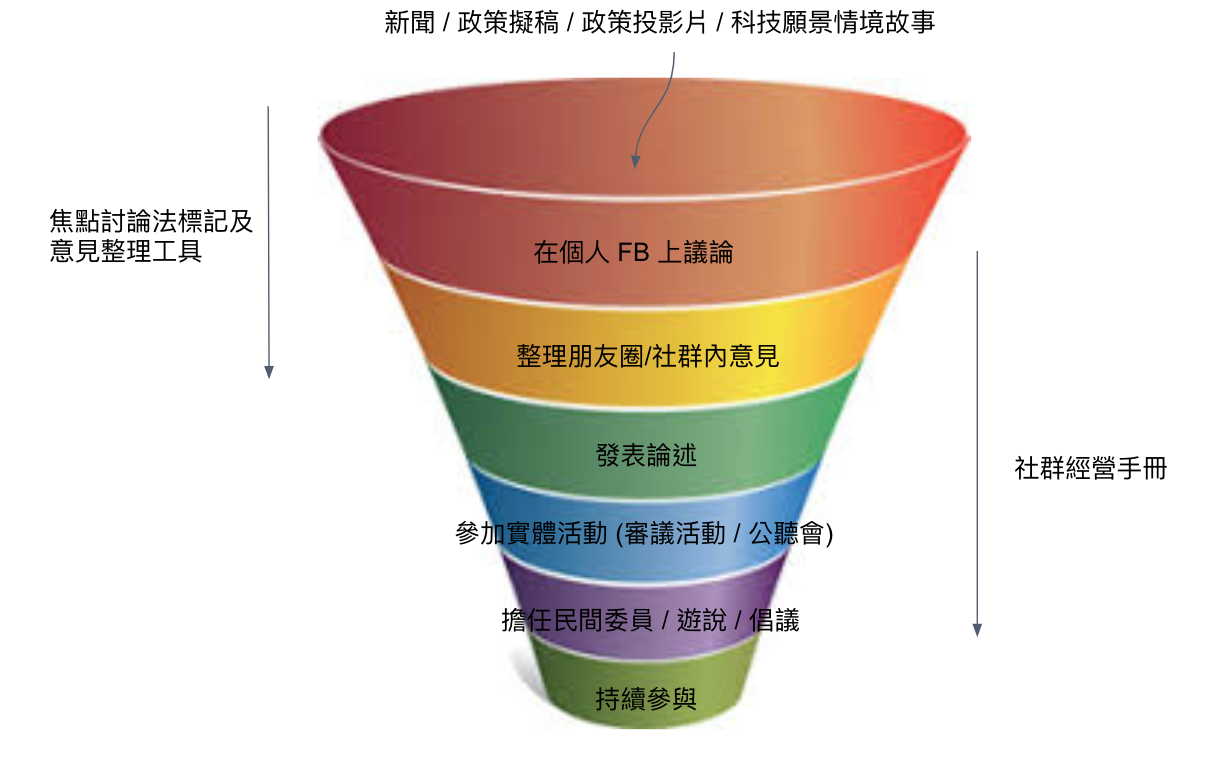
\includegraphics[width=.9\linewidth]{./images/participation_funnel.png}
\caption{\label{fig:org10ad05c}
行動參與深度圖}
\end{figure}
\section{研究目的}
\label{sec:org505933c}
依據上述背景與核心問題,本研究目的分為兩個層面,簡述如下:
\begin{enumerate}
\item 研析既有網路參與機制,找出網路社群參與之核心問題。
\item 設計一套適用「數位原民」非同步的網路討論方式提升議題討論的品質與參與政策過程的深入程度,並促使網路社群自組織議題社群增加議事資本。
\end{enumerate}
\section{研究方法 }
\label{sec:orgf909871}
\subsection{研究架構}
\label{sec:org3fa8628}
\begin{figure}[htbp]
\centering

\includegraphics[width=.9\linewidth]{./images/research_arch.png}
\caption{\label{fig:orgfed04cc}
研究架構}
\end{figure}

\subsection{研究流程}
\label{sec:orge6b3b0e}
採用 Double Diamond \cite{double_diamond} 設計流程的四個階段作為設計發展的介紹綱要 \ref{fig:double-diamond} 。

\begin{figure}[htbp]
\centering
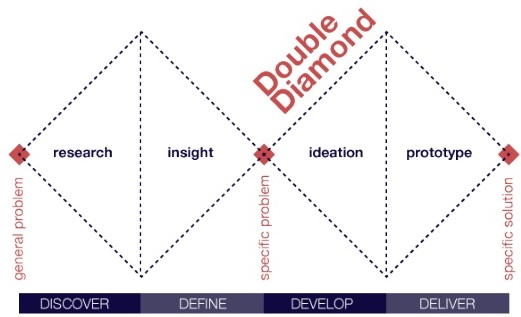
\includegraphics[width=.9\linewidth]{./images/Double-diamond-process.jpg}
\caption{\label{fig:org70edbd5}
"Double Diamond Process - CC BY 4.0 International Olga Carreras Montoto" from \url{https://commons.wikimedia.org/wiki/File:Double-diamond-process.jpg}}
\end{figure}

本研究架構之第一部分與第二部分分別對應到前後兩個階段,每個階段採取不同的工具協助發展該階段的探索/執行目標:

\begin{enumerate}
\item 網路社群視角之科技政策參與機制分析
\begin{itemize}
\item 發現(Discover)
\item 透過使用者訪談對象挖掘並整理出的重點功能/溝通中重要的協作模式以及其原因,過程裡的重點整理在服務藍圖、顧客旅程等幾個大項目裡。
\begin{itemize}
\item 定義(Define)
\end{itemize}
\item 設計敏捷方法定義關鍵問題與關鍵環節。
\end{itemize}
\item 線上線下整合網路參與機制設計開發與驗證
\begin{itemize}
\item 開發(Develop)
\item 原型測試
\item 交付(Deliver):產品實際使用
\end{itemize}
\end{enumerate}

所開發之成果如 \ref{fig:research_flow} 所示反覆循環驗證。
\begin{figure}[htbp]
\centering
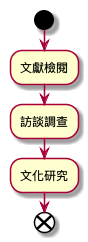
\includegraphics[width=.9\linewidth]{./images/research_flow.png}
\caption{\label{fig:org7e1c5fc}
研究流程}
\end{figure}
\subsection{網路社群視角之科技政策參與機制分析}
\label{sec:org4c6eac5}
\begin{enumerate}
\item 文獻檢閱
\label{sec:org688e25f}
文獻檢閱主要為國內外網路參與機制、如何提升網路言論品質、網路社群作為利害關係人三大部分,與服務設計中的使用者經驗設計作為開發解決方案之主要方法論。在期刊文獻專著之外,本研究大量參考網路社群原生之文本、使用者中心之產品開發設計,目的為產出可促進「數位原民 」討論品質之實用產品或服務為目的。
\item 使用者訪談
\label{sec:org207a54a}
以「滾雪球抽樣」(snowball sampling)方式,在網路資訊社群參與科技政策的流程中,會參與的不同角色之人員進行訪談,涵括「積極公民(active citizen)」、NGO 工作者、網路社群專家、政策分析師、審議主持人、政黨智庫、法人承辦、部會幕僚、高層事務官、外部顧問、政務官等,以此為依據產出使用者畫像(persona)、服務藍圖(service blueprint)、顧客旅程圖(customer journey map)、用途故事(Job Story)等使用者經驗分析,挖掘既有科技政策形成與網路參與機制中溝通落差的痛點與待解問題,從而設計試作線上線下整合線上參與機制後,進一步拿產品做使用者測試。

本研究主要透過訪談回顧歷年網路公民參與機制的設計與困難,部分受訪者選擇匿名不公開。 訪談日期形式、訪綱見附錄。
\item 設計敏捷方法
\label{sec:org081d66e}
設計敏捷方法 (Design Sprint Method)\cite{jake16} 是由 Google 提出並且於內部實踐受到歡迎。概念基礎來自於敏捷開發(Agile)、設計思考(Design Thinking)與革新遊戲法(Gamestorming)。讓團隊在五天內定義關鍵問題和目標、大量發想產品解法、決定發展方向、做出原型、使用者測試。(須改寫或標註引用來源)五天的 Design Sprint 適合團隊一起挑戰高風險的問題,並且願意從新的角度思考產品,在最短的時間內完整發想又驗證產品構想。比一兩天的工作坊更能完整盤點想法並實際動手測試,又不需等待一個月的開發期才能做使用者驗證。

本研究使用這個方法探索「 \textbf{科技政策如何在前期規劃納入更多民間專家的建設性意見} 」的可能性方案。本團隊則依團隊狀況微調工作坊進行形式,以下為微調形式。

週一團隊選擇要解決問題的關鍵節點,並安排週五的受試者,目的是為了找出問題關鍵,之後的點子發想與原型才能切合問題。
\begin{enumerate}
\item 列出現有服務的 actor 如何達到想要的關鍵結果的流程,視覺化在白板上
\item 邀請 3 位外部專家讓團隊詢問這個流程中會遇到什麼問題,用以修正該張流程圖,中間團隊成員會一邊聽外部專家分享一邊寫下 How might we 筆記,結束後分享並貼到流程圖上
\item 團隊成員投票選擇解決問題的關鍵節點
\item 找到關鍵節點後,列出要驗證的關鍵問題(sprint question)
\item 安排週五的受試者。
\end{enumerate}

週二發想點子,強調 inspiration 和個人深度思考。
\begin{enumerate}
\item Lightning Demo :針對前一天找出的關鍵節點和關鍵問題,首先做 Lightning Demo,讓團隊成員分享值得借鏡的好點子,並且以圖像化的方式將這些概念記錄在白板上。
\item Crazy 8:下午則會讓團隊成員各自發想點子,並且要求快速針對每個點子產生八個變體
\item Solution Sketch:最後將想法收斂做成三格式的解決方案,並且為每個解決方案取名與加上說明文字,將會在週三匿名展示讓團隊討論。
\end{enumerate}

週三要決定要測試的解決方案,花一天來決定。
\begin{enumerate}
\item Art museum:全部掛在牆上,不解釋是哪個人的想法,有疑問寫便條紙貼在概念下方。
\item Heat map:用小點點投票
\item Speed critique:
\begin{enumerate}
\item 每個 sketch 3 分鐘快速討論
\item 用便利貼紀錄概念中突出的點、擔心的點,貼在概念上方。
\item 加入六頂思考帽,指定團隊美人分別擔任樂觀者、悲觀者、技術專家、使用者專家、點子王與陰謀論者,以刺激多元觀點討論
\end{enumerate}
\item 一開始原作者不解釋,最後再解釋
\item straw poll(10 min-20 min):
\begin{enumerate}
\item 一人一票(大點點) 一人解釋一分鐘
\item supervote:Decider 最後決定權:三票
\end{enumerate}
\item StoryBoard:以故事畫面的方式,畫出使用者使用待被驗證的解決方案之流程,作為週四原型開發之使用者情境依據。
\end{enumerate}

週四專心做原型開發(Prototyping)。
\begin{enumerate}
\item Fake it,看起來夠真即可。
\item 團隊分工製作原型。
\item 實際演練測試訪談問題與測試情境。
\end{enumerate}

第五天做使用者驗證
\begin{enumerate}
\item 測試五個使用者
\item 除了訪談團隊外,需直播讓其他團隊成員觀看並且記下觀察到的反應。
\item Look for pattern
\end{enumerate}
\item 服務藍圖
\label{sec:orgd22ff10}
服務藍圖是一套以圖表形式呈現目標對象經歷一串(服務)流程中,整體環境中的各項互動因子間互動模式、接觸點、關係人角色與其他參與人員盤點出來的設計工具。1984 年 Shostack 在哈佛商業評論提出以服務藍圖檢視服務產出之過程 \citep{shostack1984} 。服務藍圖幫助我們釐清整個過程中,每個參與人員扮演的角色、執行的動作、接觸的工具、互動的模式。透過服務藍圖工具,我們可以視覺化目標對象在做議題倡議時經歷的過程,幫助我們看到倡議民眾在過程中的哪些環節上遇到困難,並提出對應的改善方案。
\item 顧客旅程圖
\label{sec:org3ffb2e3}
顧客旅程圖相較於服務藍圖,能讓過程中的接觸點看得到,並對觸點作評估管理。顧客旅程圖與服務藍圖不同之處在於,顧客旅程圖聚焦的範圍目標放在顧客在流程裡執行的動作與執行動作的接觸點上。除了詳細盤點觸點之外,同時也會考慮顧客在每個「行動」甚至「關鍵時刻」時的「目標」、「動機」、「情緒感受」,從釐清每個動作的動機目標與執行時的感受,讓我們能以客觀的視角,找到改善流程的著力點。
\end{enumerate}

\subsection{線上線下整合網路參與機制設計開發與驗證 }
\label{sec:orgb1ca101}
以前述使用者經驗設計的訪調與分析為基礎,滾動式設計開發線上線下整合網路參與機制,捨棄傳統瀑布流開發方式,使用網路業快速回應使用者需求常用的敏捷開發法(agile development) \cite{agile_development} ,透過使用者驗證不斷調整產品開發方向,避免按照一年前制定的規格一路做下去最後才發現不符合實際使用者需求。

本團隊亦將所設計之解決方案皆開源(open source),讓公眾亦可加入開發、散佈、改作,並且架設協作平台讓網路社群得以參與機制之開發與回饋。
\begin{enumerate}
\item 精實創業與敏捷開發以滾動式修正
\label{sec:org61fe0cc}
在設計開發線上線下整合網路參與機制中,本團隊遵循敏捷開發宣言 \cite{agile_development} :

\begin{verse}
藉著親自並協助他人進行軟體開發,我們正致力於發掘更優良的軟體開發方法。透過這樣的努力,我們已建立以下價值觀:\\
\vspace*{1em}
個人與互動 重於 流程與工具\\
可用的軟體 重於 詳盡的文件\\
與客戶合作 重於 合約協商\\
回應變化   重於 遵循計劃\\
\vspace*{1em}
也就是說,雖然右側項目有其價值,但我們更重視左側項目。\\
\end{verse}

在不斷回應變化與跟使用者合作的參與機制開發中,本團隊亦參考「精實創業」 \cite{lai17_jing} 一書中最小可行性產品(Minimal Valuable Product,MVP)、使用者測試驗證產品假說之概念,在產品開發初期即製作原型測試(prototype testing),並且開發最小可行性產品後即推出讓使用者測試,根據使用者回饋不斷修改產品功能與參與機制設計。

此回饋修正週期為兩個禮拜,採取 「SCRUM」\cite{sutherland18_scrum} 開發模式,採取兩個禮拜為一個衝刺週期(sprint)的方式,每個衝刺週期由團隊一起回顧驗收上個衝刺週期的成果、使用者回饋與改善工作流程開始,接著依產品負責人排定的產品開發需求,由開發人員評估工作量與分配工作,在一個衝刺週期中「排定的事項不能改變,也不能再加入東西。團隊必須要在衝刺期間自主工作,以完成自己預測可完成的事項。」\citep[p. 328]{sutherland18_scrum} 每個衝刺週期須交付使用者具有價值的產出,詳細開發進度可見團隊在 GitHub 上 Milestone 的工作記錄。\footnote{本團隊開發進度紀錄請見\url{https://github.com/SenseTW/sensetw/milestones}。}
\item 開源社群參與
\label{sec:orgb3a37d6}
本團隊所設計開發的解決方案亦為開源(open source),在開發過程中即將所開發的程式碼、圖像介面設計、公開文字產出(部分訪談內容、部落格、數位原民參與手冊)、介紹影片等,以開放授權方式公開在網路上讓任何人可散佈、改作。本團隊並且與網路社群共同協作,在 GitHub 平台公開開發進與收集問題回報,在 g0v 臺灣零時政府社群\footnote{「g0v.tw 是一個推動資訊透明化的社群,致力於開發公民參與社會的資訊平台與工具。」(\url{https://g0v.tw/zh-TW/about.html})。}的 Slack 討論平台上讓任何人可加入開發相關討論,並線下參與 g0v 黑客松與其年會、參與 COSCUP\footnote{「開源人年會起源於2006年,是由台灣開放原始碼社群聯合推動的年度研討會,也是台灣自由軟體運動重要的推動者之一。此活動通常一連兩日,包括有講座、攤位、社團同樂會等。除了邀請國際的重量級演講者之外,台灣本土的自由軟體推動者也經常在此發表演說,會議的發起人、工作人員與講者都是志願參與的志工。」,介紹詳見 \url{https://en.wikipedia.org/wiki/COSCUP}。} 開源人年會等活動與網路社群交流共同協作。並以集客式行銷(inbound marketing)方式撰寫部落格,以吸引對此線上線下整合網路參與機制有興趣之網路閱聽眾,參與協作開發與使用。

協作入口:
\begin{itemize}
\item 即時訊息討論: \url{https://join.g0v.tw} , channel \#sense;討論紀錄:\url{https://g0v-slack-archive.g0v.ronny.tw/index/channel/C7D8SL96V}
\item 專案開發: \url{https://github.com/SenseTW}
\item 電子郵件群組: \url{https://groups.google.com/d/forum/sensetw}
\end{itemize}

\begin{table}[htbp]
\caption{\label{tab:org28597bf}
著作物列表}
\centering
\rowcolors[]{2}{contiYellow!5}{contiYellow!20}
\begin{tabular}{l|p{110pt}|p{110pt}}
\toprule
著作物 & 連結 & 授權\\
\midrule
sense.tw 程式碼與介面設計 & \url{https://github.com/SenseTW/sensetw/} & MIT\footnotemark\\
數位原民參與手冊 & \url{https://sense.gitbook.io/guides/} & CC BY-SA 3.0 台灣- 財團法人開放文化基金會\footnotemark\\
部落格 & \url{https://medium.com/sense-tw/} & CC BY-SA 4.0 International\footnotemark\\
\bottomrule
\end{tabular}
\end{table}\footnotetext[4]{\label{orgaec4faa}MIT 授權允許被授權人「有權利使用、複製、修改、合併、出版發行、散布、再授權和/或販售軟體及軟體的副本,及授予被供應人同等權利,惟服從以下義務:『在軟體和軟體的所有副本中都必須包含以上著作權聲明和本許可聲明。』」,中文說明 2018 年 12 月 22 日摘自維基百科\url{https://zh.wikipedia.org/wiki/MIT\%E8\%A8\%B1\%E5\%8F\%AF\%E8\%AD\%89},英文 MIT 協定全文請見:\url{https://opensource.org/licenses/MIT}。}\footnotetext[5]{\label{orga27fac0}CC BY-SA(姓名標示-相同方式分享) 3.0 台灣之授權條款為依據「創用 CC 公眾授權條款」中授權姓名標示─相同方式分享。本授權條款允許使用者重製、散布、傳輸以及修改著作(包括商業性利用)。若使用者修改該著作時,僅得依本授權條款或與本授權條款類似者來散布該衍生作品。使用時必須按照著作人指定的方式表彰其姓名。詳細授權條款請見:\url{https://creativecommons.org/licenses/by-sa/3.0/tw/legalcode}}\footnotetext[6]{\label{org63f6a50}CC BY-SA 4.0 (Attribution-Sharealike) International,詳細英文授權條款請見:\url{https://creativecommons.org/licenses/by-sa/4.0/}。}
\end{enumerate}

\section{文獻檢閱 }
\label{sec:orgf96339f}
本章回顧「科技治理體系及溝通缺口」、「線上公民與政治參與的要素」以及「數位工具的幫助與限制」作為研究背景。
\subsection{科技治理體系及溝通缺口 }
\label{sec:org8d7605e}
為設計適合使「數位原民 」、科技社群參與政策討論的線上機制,並回應進入場域所必須回答的問題,例如「什麼是科技政策?」、「科技政策怎麼來的?」、「科技會報跟科技部差在哪邊?」、「哪邊可以看到科技發展藍圖(Road Map)跟現在有哪些計畫在推動)等等,及了解基本政策過程,接下來以民間視角綜合整理,恐有未盡之處或錯誤,仍以政府公告為主。

我國科技政策基本上是依據「科技基本法」所規定的「政府每四年召開『全國科技發展會議』,透過事前與中央科技機關確定相關議題,訂定議題內容主責範圍,再參酌產官學研意見與民間團體溝通,經召開全國科技發展會議討論後,提出『國家科學技術發展計畫』,報請行政院核定後,作為我國未來四年主要科技政策與推動科技研究發展之依據」。 \citep*{guo17} ,較為重要的有三個類型的會議,分別為「全國科技會議」、「全國科技顧問會議」、「產業發展策略會議」。

\begin{figure}[htbp]
\centering
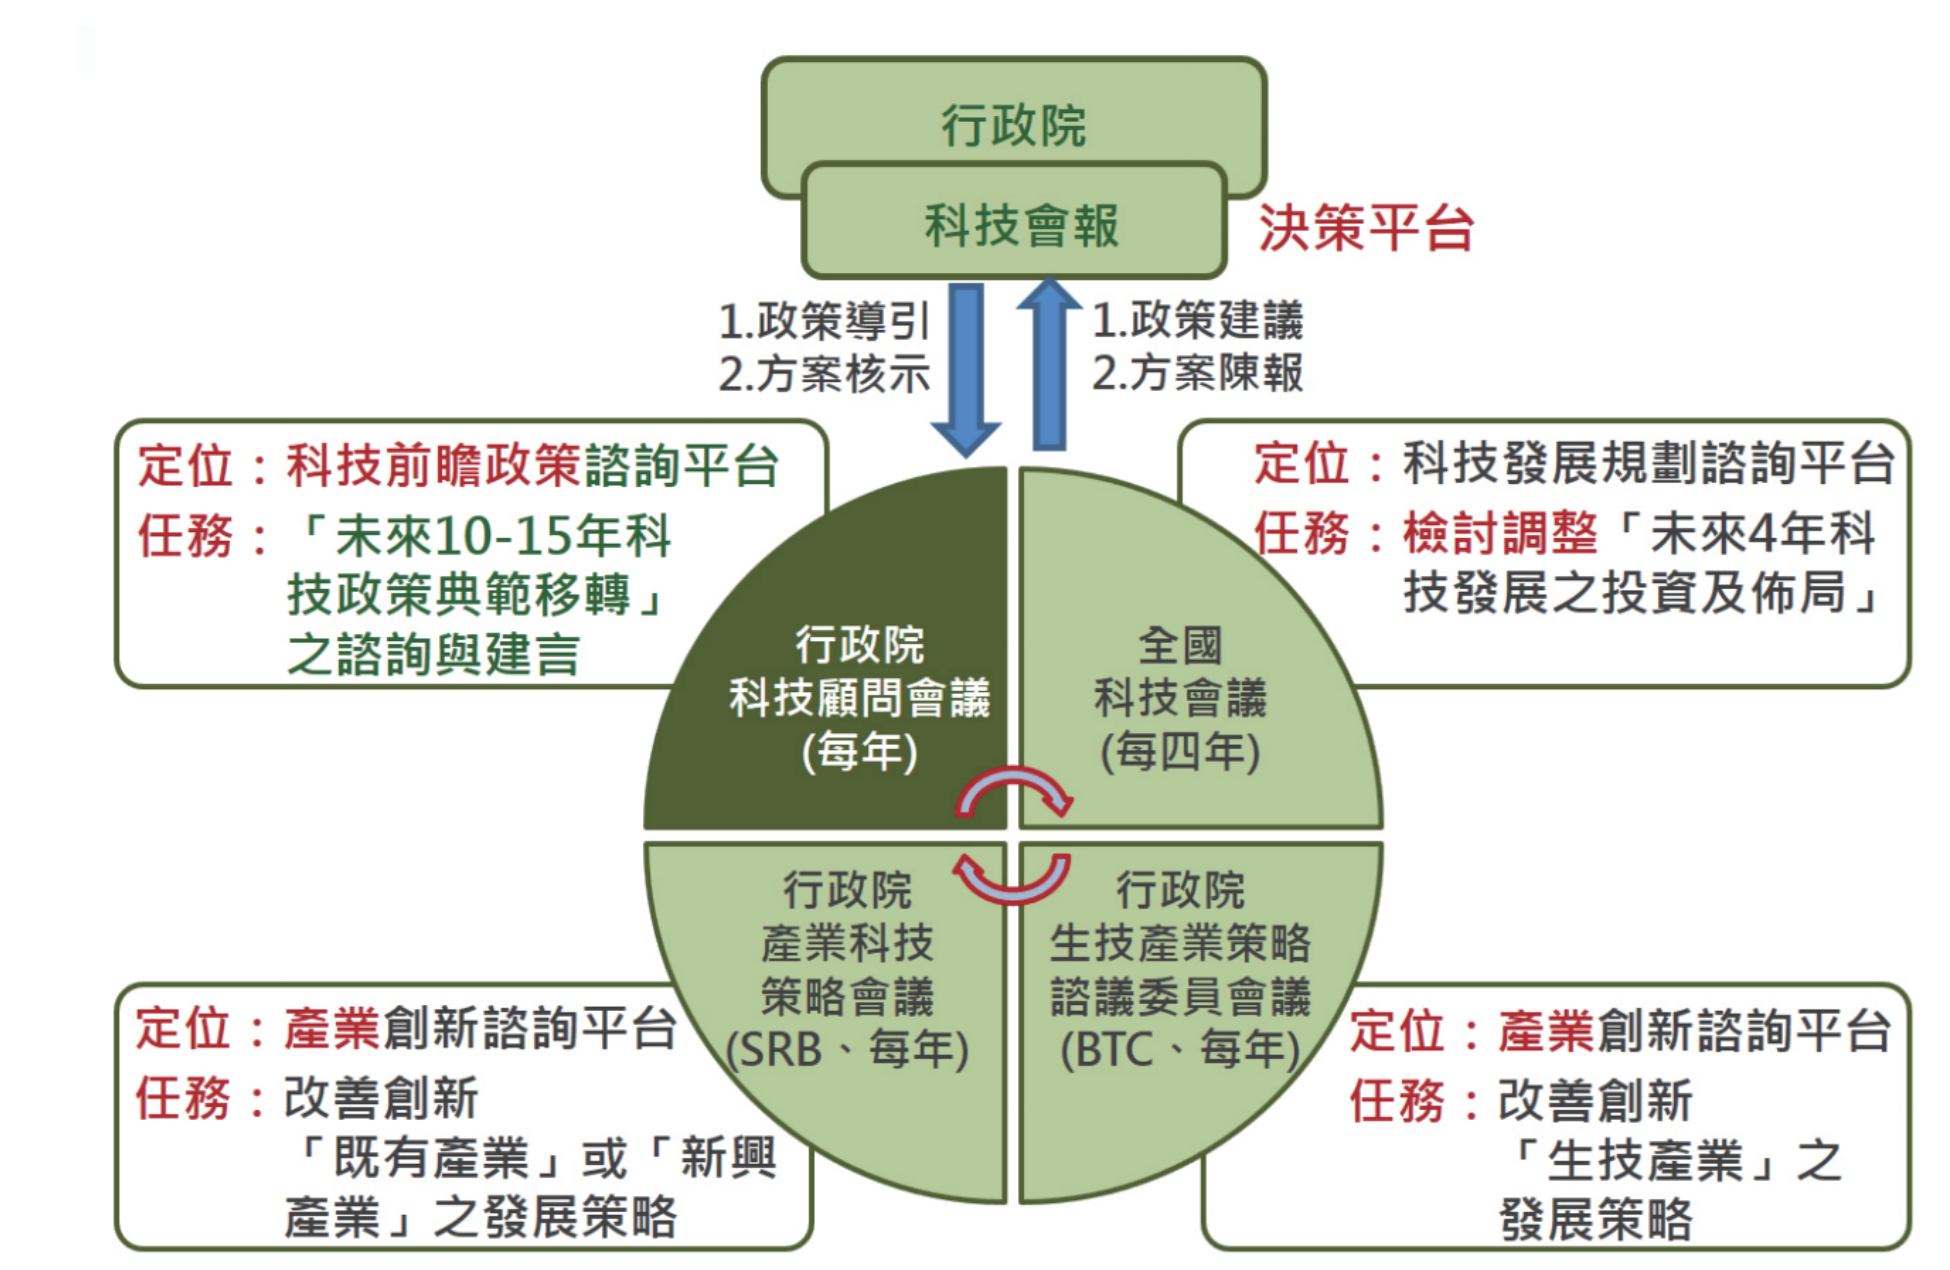
\includegraphics[width=.9\linewidth]{./images/tech-gov-framwork.png}
\caption{\label{fig:org5e329b4}
我國重要科技會議平臺會議運作機制(行政院科技會報辦公室製圖,來源:\citep*{guo17})}
\end{figure}
\begin{enumerate}
\item 全國科技會議
\label{sec:org3924b0a}
依據「科技基本法」每四年舉辦的全國科學技術會議,做為未來國家科技發展藍圖,2016 年遭前台灣積體電路董事長張忠謀認為缺少產業界聲音,批評淪為形式上的大拜拜。陽明大學生物醫學影像暨放射科學系教授高怡宣則認為近二十年的會議都改由大官報告及做結論,缺乏真正的腦力激盪跟討論,讓學界和產業界都失去熱情,國家科技發展也失去方向。
\item 科技顧問會議
\label{sec:orgd72c28e}
行政院科技顧問會議之前身,最後一次舉行的「科技顧問會議」為 2011 年。科技會報原訂 2018 年開始重新啟動「科技顧問會議」,每年召開 一次聘請國內外專家擔任顧問,產出「科技顧問會議建言書」作為重要科技會議之政策參考,但並未舉行。
\item 產業發展策略會議
\label{sec:org7398fab}
「產業科技策略會議(Strategy Review Board, SRB)以及行政院生技產業策略諮議委員會議(BioTaiwan Committee, BTC),透過整合國際情
勢、政府施政與產業趨勢等方向,與產官學研各界進行特定議題討論,相關結論做為產業科技推動的重要依據。」\citep*{guo17}
\item 相關單位
\label{sec:org59c10b7}
科技政策相關的單位主要是科技會報、科技部。科技會報在組織定位上為跨部會協調、國內科技政策智庫的整合平台,以及行政院院長之科技決策幕僚單位,掌管 \textbf{國家科技資源 1000 億之分配} 。科技部前身則為 1959 年成立的行政院國家科學委員會,推動科學技術發展的專責機構,主要任務推動全國整體科技發展、支援學術研究,以及發展科學園區。
兩者因涉及業務領域廣泛,且限於編制員額與領域專長,多從相關專業法人單位借調人才協助或另行成立財團法人\footnote{常有法人現階段功能待檢討或疊床架屋案例,不乏社會與論批評。}。
\item 科技計畫
\label{sec:org4e29bf2}
政策的施行主要是以計畫的形式推動,也是民眾最有感,除了「社會議題」(society issue)外較易被討論的主題。現階段科技會報管考科技部之科技計畫,科技部管考其餘部會之科技計畫\footnote{資訊來源:數位政務委員唐鳳。 2018 vTaiwan 小聚取得。}, \ref{tbl:tech-project-information-sources} 列出民眾可以查找分散在各部會科技計畫的資訊來源。

\begin{table}[htbp]
\caption{\label{tab:org6878d0a}
各部會轄下科技計畫資訊來源(資策會產業發展所製表)}
\centering
\begin{tabular}{lll}
\toprule
部會 & 局處司室組 & 資訊來源\\
\midrule
內政部 & 秘書室 & 研究發展知識平台\\
國防部 & 資源規劃司 & 業務統計及研究報告、軍事期刊\\
法務部 & 綜合規劃司 & 法務研究計畫與成果、 犯罪防治研究資料庫\\
經濟部 & 技術處 & 文宣刊物\\
交通部 & 科技顧問室 & 科技研究、交通年鑑\\
勞動部 & 勞動及職業安全衛生研究所 & 研究成果、勞工安全衛生研究年報\\
原能會 & 核能研究所 & 年報、GRB 政府研究資訊系統(需自行搜索)\\
農委會 & 科技處 & 農業計畫管理系統\\
衛服部 & 科技發展組 & GRB 政府研究資訊系統\\
環保署 & 永續發展室 & 環保專案成果報告資訊系統\\
科技部 & 前瞻及應用科技司 & 科技部出版品、 國內學術電子期刊系統\\
\bottomrule
\end{tabular}
\end{table}
\item 成為沈默輸家的資訊科技社群
\label{sec:org17a8c2f}
自 2014 舉辦的\href{https://www.ndc.gov.tw/Content\_List.aspx?n=F6A29549FD03E057}{經貿國是會議} 以來、公部門們常常提到「科技社群」,但似乎並無精確定義,按筆者個人經驗,目前只見 2017 年的開源人年會中的\href{https://www.youtube.com/watch?v=mrMsNItdkNs}{南部社群與法人協作}演講中提到「科技社群」四字,而從科技部的相關計畫:科技社群建構:新興科技產業相關議題之研究,可發現學者所想像的社群是某種由上而下建構的平台,而非由下往上自組凝聚的人民團體。因此接下來本研究會試圖釐清所謂的「科技社群」為何,另外需特別強調的是,這裡提及的社群 (community) 一詞與社區營造裡的社區 (community) 為不同指涉對象。

沒有人可以代表「網路」,在網路上每個人都是各自獨立的節點,只是有些人是比較大的節點,認識更多人、傳遞更多資訊,通常被稱之為意見領袖(Key Opinion Leader)。意見領袖並非他想做什麼,下面就會有網軍群起跟隨,KOL 指的比較偏向網路上某一社群內有影響力的人,較像是一個跟社群溝通的窗口,是因為他在社群內的專業與參與付出而有影響力且受信任。

不同於傳統公協會或是人民團體,網路社群因為興趣和共同關注議題而聚集,成員可能跨地域、跨職業,也沒有成立正式的法人組織,但是這個社群因為共同的承諾參與、默契、工具凝聚在一起,持續在網路上活躍,而成員對這個社群產生了歸屬感。例如攝影同好、動漫社群、寫程式的社群,可能在不同的論壇、通訊工具上討論相關話題,分享新知與作品。Etienne Wenger(2003)稱呼這類通過對特殊活動或興趣分享專業技術和激情而聚在一起的群體為「實踐社群」(community of practice)。

「實踐社群」這樣崇尚實作的文化,使得一個人在這樣的社群的影響力是建立在他為社群貢獻過什麼事蹟,因此網路的暱稱 ID  比本名還真,基本上可以算在江湖 (community) 的藝名 (nickname),任何職銜在此也不重要,大家認可的是該人做過的貢獻,而不是他是否為理事長、發起人。社群所形成的文化,也就是所謂的默契,會讓社群的意見領袖,受到一定程度的規範,若是意見領袖打破這個默契,就會在所屬的社群中影響力下降。這樣的治理模型在自由開源社群特別常見:「仁慈的獨裁者」(benevolent dictator)\textsuperscript{\ref{org63f6a50}} 必須保持仁慈,否則巨大的分歧會導致專案被復刻(fork)並由新的領導所掌管。這也是接下來建議一章會看到受訪者希望專家會議內容公開,因為他們無法代表他們所屬的社群,基於跟社群的默契,他們需要讓社群裡的更多人可以一同參與跟政府的討論並給意見。

除了「實踐社群」外,網路上也有專注在討論特定社會議題的社群,成員可能是「積極公民」、學者或有官職身份者等等。每個網路社群習慣的討論平台也會不同,可能在 Facebook、Instagram、Line、Telegram、Twitter、Slack、IRC、PTT 等不同的工具平台上。本研究將此類社群稱之「議題社群」。隨著議題發酵的熱度,議題社群可能採取倡議、遊說、陳抗等等不同行動策略試圖影響政策。
綜上述,大致上網路社群有兩種生命週期,一種是以興趣為導向,以實作和數位資產為基礎的實踐社群,以開源社群為例;另一種是議題導向的倡議社群,例如從關注特定議題的粉絲頁到發起遊行抗議。許多社群至凝聚期時已有相當影響力與網路聲量,卻因行政成本考量不一定會走到有法人形式的營運期,造成這些社群的聲音很難被納入政策諮詢過程中,也無法有明確的組織授權任何人代表那個社群。
\begin{enumerate}
\item 實踐社群
\label{sec:org2b38a46}
\begin{table}[htbp]
\caption{\label{tab:org0f4e7f9}
實踐社群的生命週期}
\centering
\rowcolors[]{2}{contiYellow!5}{contiYellow!20} \footnotesize \setlength{\tabcolsep}{3pt}
\begin{tabular}{lp{80pt}llp{86pt}p{86pt}}
\toprule
特性/階段 & 萌芽期 & 發起期 & 凝聚期 & 擴大推廣期 & 營運期\\
\midrule
關鍵活動 & 網路上分享特定知識 & 共有數位資產 & 定期實體聚會 & 定期大型活動 & 成立人民團體\\
誰能代表 & 無 & 發起人 & 無 & 無 & 不同案例有不通狀況\\
自治條例 & 無 & 無 & 有 & 有 & 有\\
營運成本 & 極低 & 低 & 中 & 高 & 極高\\
案例 &  &  &  & COSCUP、MOPCON、 & 開放文化基金會 、自由軟體協會\\
\bottomrule
\end{tabular}
\end{table}
\item 議題社群
\label{sec:orgb039e15}
\begin{table}[htbp]
\caption{\label{tab:org7fd19b7}
議題社群的生命週期}
\centering
\rowcolors[]{2}{contiYellow!5}{contiYellow!20} \footnotesize \setlength{\tabcolsep}{3pt}
\begin{tabular}{llp{80pt}p{80pt}p{80pt}p{80pt}}
\toprule
特性/階段 & 萌芽期 & 發起期 & 凝聚期 & 擴大推廣期 & 營運期\\
\midrule
關鍵活動 & 罵文/釐清議題 & 分享相關政策/報導/學術文獻、成立粉絲頁、群組 & 定期讀書會/行動策略討論 & 倡議/遊說/開記者會/遊行等等定期大型活動 & 協會/基金會\\
誰能代表 & 無 & 發起人 & 無 & JOIN 提案者 & 董事長/理事長\\
自治條例 & 無 & 無 & 有 & 有 & 有\\
營運成本 & 極低 & 低 & 中 & 高 & 極高\\
案例 &  &  &  & COSCUP、MOPCON、 & 開放文化基金會 、自由軟體協會\\
\bottomrule
\end{tabular}
\end{table}
\end{enumerate}
\item 溝通缺口
\label{sec:org88550d7}
這類型會議主要有「三個『溝通缺口』,分別是誰能出席、誰被排除的『代表性缺口』;與會人士知識/ 語彙的落差;不同參與者,在議程設定與結論綜整時的權力不對等」\citep*{alberttzeng08},
其中「知識/語彙的落差」由全國性會議的舉辦形式造成。類似的「經貿國是會議」八成的時間只能讓參與者宣讀自己想說的意見,而非實質性的對話討論。「大費周章動員上百人辦這一場線下會議,卻把多數時間用於書面(或網路)能完成的事,不禁令人惋惜。特別是,這些紛呈的意見中,其實充斥著價值上的對立(例如對勞動條件、稅率的看法),或施政優先順序上的角力,卻都沒辦法被充分展開,在對質與辯證獲得進一步釐清,造成會議充斥著「貌似多元、實則淺碟」的內容。」\citep*{albert2014} 。
\texttt{說明知識落差的原因}
則指出造成數位原民、資訊科技社群與政府部門的「知識/語彙的落差」之主要問題是資訊來源不同、做事文化不同以及政府部門認知頻寬匱乏,沒有精力
\end{enumerate}
\subsection{線上公民與政治參與的要素}
\label{sec:org1a26084}
新型態的網路公民參與是主張利用網路與電子媒體的即時連結特性,透過共同協力的方式來影響政府的決策,採廣義認定的「政治參與」的定義下,網路上的公民參與即是政治參與,可區分為四類,包括:(1)代議民主式參與(participation  in  representative  democracy),如線上投票(2)直接民主式參與(participation  in  direct  democracy),如參與式預算與線上連署(3)審議式民主參與(deliberative participation)則強調政府與民眾雙向互動與溝通,如線上論壇、(4) 示威式民主參與(demonstrative democracy)\citep*{chen16} ,而影響線上公民參與的因素有九個構面,見表 \ref{tbl:online-participition} 。

\begin{table}[htbp]
\caption{\label{tab:orgce01001}
影響線上公民參與的九大構面 - 資訊來源:(Macintosh 2004)}
\centering
\begin{tabular}{ll}
\toprule
參與程度 & 影響線上公民參與的九大構面\\
\midrule
參與成員 & 公民參與了「什麼」?程度為何?\\
納入公民參與的時機 & 「誰」參與了這些活動?\\
使用的科技工具 & 「如何」讓公民進行參與活動?「什麼」樣的科技工具可以輔助?\\
參與規則 & 「什麼」樣的個人資訊需要被收集?\\
參與時間 & 公民參與的時間有「多久」?\\
參與規模 & 「多少」公民參與?  從「哪裡」參與?\\
參與成本 & 參與的成本有「多少」?「如何」宣傳?\\
參與結果 & 從政治、法律、文化、經濟、科技等面向評估參與的結果\\
\bottomrule
\end{tabular}
\end{table}

然而前述的九大構面缺少了參與誘因,\citep*{wang17}  認為觀察民眾的「政治信任感」(political trust)以及「政治效能感」(political efficiency),兩種政治態度或可預線上線下參與的行為模式,並將台灣網路使用者區分為四種,見 \ref{tbl:net-user-category} 。
結果顯示其中網路使用者以「疏離者」最多,「忠誠者」與「異議者 」參與頻率最高。因此在線上參與的最大的問題是 \textbf{沒有人要參與} ,比起機制的設計,更重要的是增加公眾參與的誘因,而誘因的設計是最為困難的。

\begin{table}[htbp]
\caption{\label{tab:org10ddd28}
網路使用者的分類(本研究再製)}
\centering
\begin{tabular}{llll}
\toprule
分類 & 定義 & 政治信任感 & 政治效能感\\
\midrule
忠誠者(Assureds) & 信任政府且認為自己能改變現況 & 高 & 高\\
異議者(Dissidents) & 不信任政府,傾向於參與較激烈的示威或抗議等社會運動以企圖改變現狀 & 低 & 高\\
從數者 (Subordinates) & 信任政府但是不認為自身有能力影響政府作為 & 高 & 低\\
疏離者(Alienateds) & 政治不值得信任也認為自己沒有改變現狀 & 低 & 低\\
\bottomrule
\end{tabular}
\end{table}

國發會近期出版的 JOIN 成果報告 \citep*{chuang18,lin18a} 也顯示出社交工具以及線下活動對於促進線上參與的重要性; 至少有七成的 JOIN 使用者在使用 JOIN 之前有參與過線下的政治公民活動,且關心的基本上都是與切身相關的議題,或是對政策表達反對意見 ; 不同年齡、教育程度,區域的公眾在「資訊近用能力」與「資訊獲取管道」上有顯著差異。因數位工具的學習門檻有相當高的排他性,使得線上能進行參與的公眾多以年輕、高教育程度,居住於都會區為主,但是很多重大爭議事件的利害關係人都不具備在網路上有足夠的理性表達能力,因此 \textbf{線上線下參與應放在一起思考而非視為兩個完全不相關的機制} ,只是對於數位原民或是資訊科技社群來而言,線上線下參與的方式與傳統審議或是專家會議舉辦方式有極大的文化落差。
 「科技改變了民眾回應的傳播方式、回應力道,特別是回應持續的時間。科技去除了兩個過去的障礙,那就是資訊的局部性及群體回應的障礙。」\citep*[p.141]{xue11_xiang}; 線上意見領袖(Keep Opnion Leader) 的政治討論頻率會影響議題異質性並間接或直接的影響其他者在線下的參與行為 \citep*{lin18b} ,使公眾能集體行動,大幅降低參與的成本以及增加議題設定(Agenda Settings)的能力,雖然 ICTs 究竟是賦予人們更多直接參與民主的權力,還是加深社會對立與分歧至今仍未見定論。

「網路適合釐清議題嗎? 網路上真的能理性對話嗎? 真的是適合作為公共討論的場域?」是「科技悲觀者」經常對線上公民與政治參與機制發出最大的質疑,ICTs 除了降低公眾對話的成本,同時也改變公眾心智並並帶來其他社會問題 \citep*{stev11} 。 \citep*{neil16} 早已指出「所有公共論述都逐漸以娛樂形式來傳達。我們的政治、宗教、新聞、體育、教育和商業,全都成為娛樂業的附庸,對此民眾多半毫無怨言,甚至漠不關心。於是,我們成為瀕臨娛樂至死的一群。」,如今在網路上的任何的政治討論最後都回到社交工具上(SNS),由於社交工具將公眾切成一個又一個的「小世界網路」\footnote{根據臉書的研究臉上使用者跟一個陌生人在網路上的距離是 3.5 個人。 \url{https://research.fb.com/three-and-a-half-degrees-of-separation/?hc\_location=ufi}} ,使得「資訊碎片化」,介面的限制也使公眾難以在上面進行完整的論述對話,要釐清議題或是理性討論漸漸變得困難,導致「網路論戰(flaming)」\citep*{wiki:flaming} 層出不窮。

資訊科技社群作為最早採用 ICTs 的族群對於「如何打網路論戰」已有許多討論; 知名黑客以及 Y-Combinator 創辦人 Paul Gram 根據網路論戰發文依照好壞、數量分為七個層次,認為引用原文指出不同意之處是提高論述品質的重要要素之一。\citep*{paul08}

\begin{figure}[htbp]
\centering
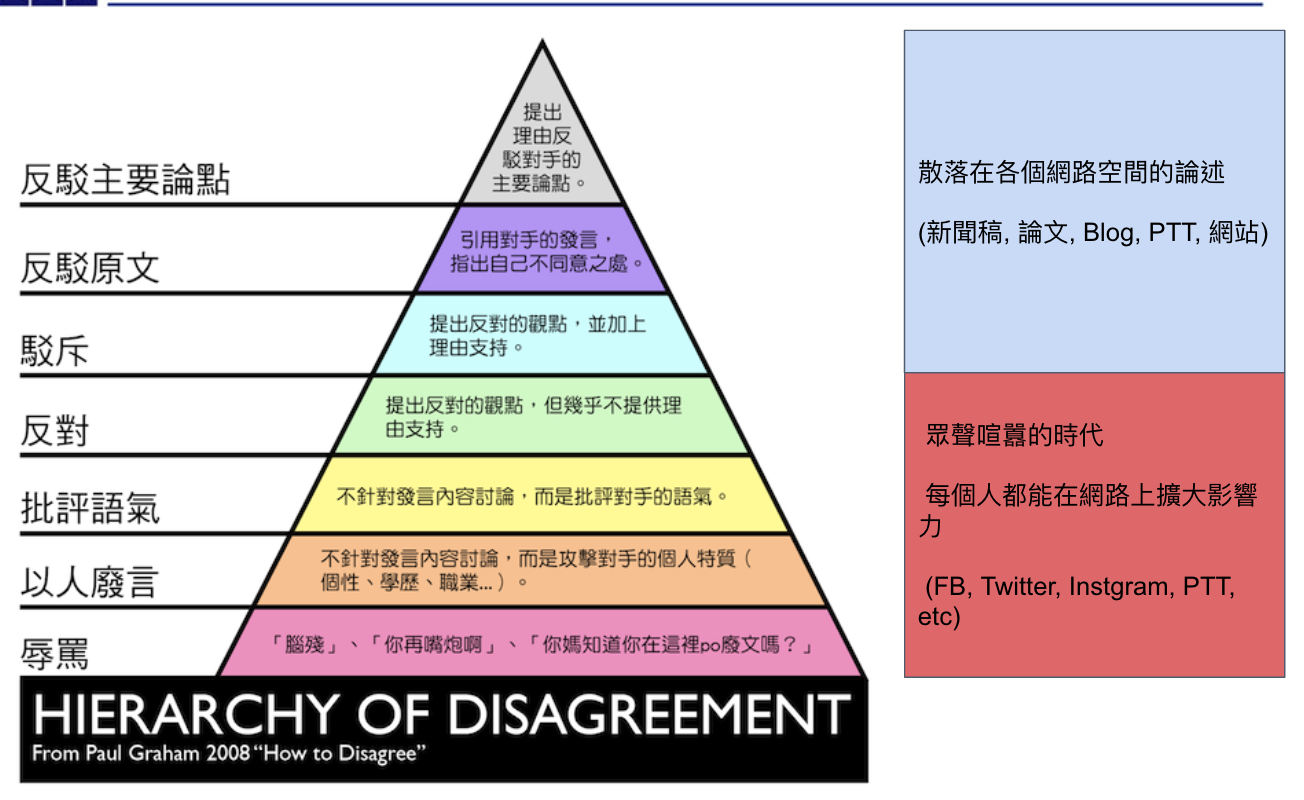
\includegraphics[width=.9\linewidth]{./images/how-to-disagree.png}
\caption{\label{fig:org189cd62}
網路論戰品質金字塔 (資料來源: \citep{zhu_2015} ,本研究重製)}
\end{figure}

若能讓參與討論的人知識越接近,越能有效對話; 控制公眾之間的「意念」流動,讓公眾在「思考」跟「探索」之間有個恰當的平衡,好的點子能更容易出現 \citep*{pentland14_shu}。 這樣在網路上發文附引言出處、資訊來源,質疑對方資訊來源這樣的文化可追朔到 BBS 時期 \citep*{malaita15}

\subsection{數位工具對參與者知識對焦的幫助與限制}
\label{sec:org0bb6b42}
長期參與 g0v.tw 設計線上審議工具,並且最後放棄開發網路審議工具的藍一婷
指出審議的數位工具最好是通用工具,也就是這個工具不會只適合特定參與機制的流程、而是可以應用在很多機制中解決特定問題,放在審議的情境,資訊工具最適合被用知情(inform)的環節,而非討論的環節 \citep{etblue18,etblue2017}。 學者 \citep*{chen08} 另外指出線上會議的效果雖相對於傳統面對面的會議,較能傳遞補充知識,讓與會者更能理性討論,產生共識的可能性較高於傳統會議,並且有參與成本低的好處,然而社會整體環境不夠成熟之前,透過線上面對面的視訊會議形式進行的「公民會議」,所有與會者的參與成本不一定會低於實體會議。

Wikipedia 以及 OpenStreetMap 的成功說明了大規模業餘公眾成果不輸於由少數菁英組成的傳統專家。
因此過往屬於研究機構才能進行政策研析的工作是否能讓公眾進行呢? \citep*{hahn16} 研究指出,透過高品質的線上資訊以及適合的數位工具,即便是困難的科技問題也能讓不具專業的新手(novice)在不了解 Big Picture 在不同階段參與,從一個範圍較大的問題開始演化,使公眾在線上問出更深層的問題,並集體產生出高品質、縱整過後的的摘要性文章。 圖 \ref{ka-process} 展示其實作之 "Knowledge Accelerator" (KA) 流程。

\begin{figure}[htbp]
\centering
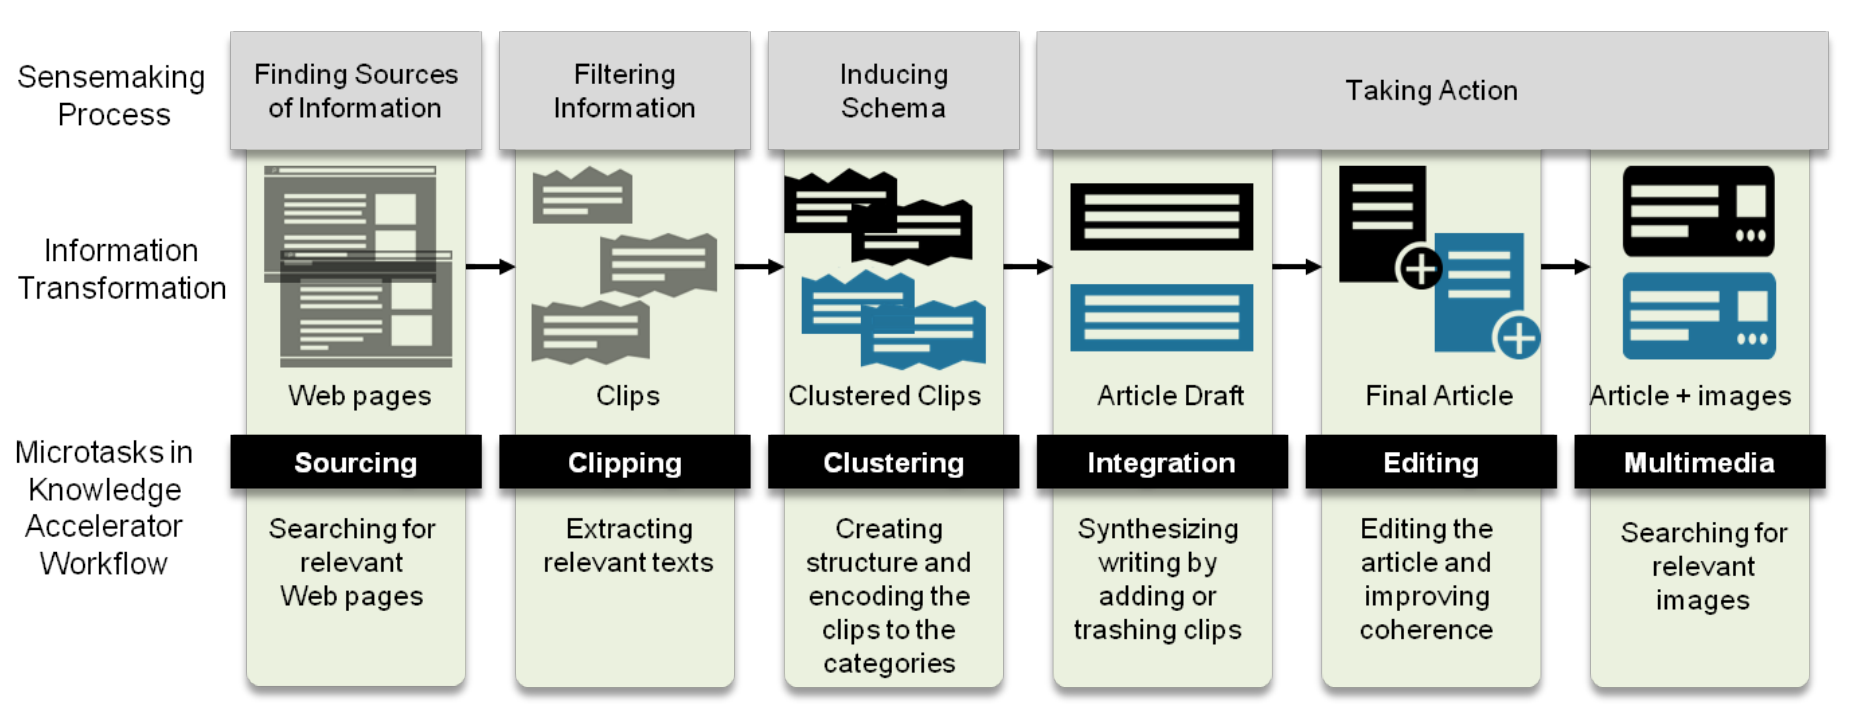
\includegraphics[width=.9\linewidth]{./images/ka-process.png}
\caption{\label{fig:org0f4b677}
The process of the Knowledge Accelerator (KA), from start to finish. 來源自: \citep{hahn16}}
\end{figure}

然而縱整過後的摘要性文章只是一種較為單向資訊呈現方式,心智圖(mind map)、概念圖(concept map)、論點圖(arguments map)被有效證明可幫助學生分析該挖掘資訊跟資訊的關係掌握新的知識 \citep*{davies10} 。 \ref{fig:kmap} 模型解釋三者主要的差別以及適合應用的時間。

\begin{figure}[htbp]
\centering
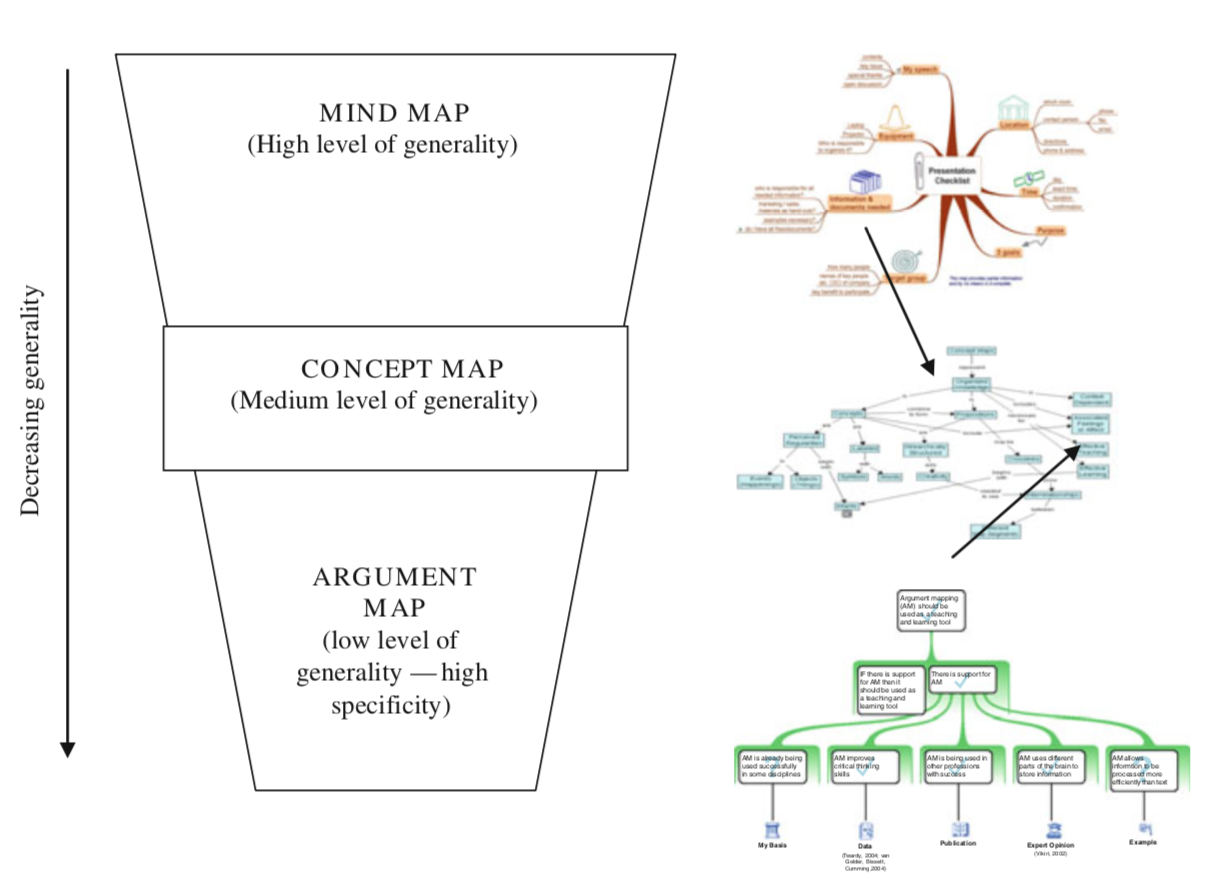
\includegraphics[width=.9\linewidth]{./images/kmap.png}
\caption{\label{fig:orgbed9a4f}
convergence of knowledge mapping technologies into a single integrated platform. from \citep*{davies10}}
\end{figure}
\subsection{小結}
\label{sec:orga330d93}
綜合上述文獻回顧可發現,若要讓公眾與政府有效溝通對話,有兩個較重要的條件需要思考:(1)如何讓公眾有更多的興趣接收政策資訊以及政治參與,(2)如何讓公眾協作進行議題釐清,從而能有足夠的政策知識與了解相關語彙與政府對話。若要促進線上參與討論,可思考(1)從意見領袖發起高頻度、低成本的政治討論會增進線上線下參與的意願,(2)在一個問題接著問更深度的問題(QBQ)和回歸原始文獻討論可增進理性討論的可能性。
\section{社群視角的科技政策參與途徑分析 }
\label{sec:orgb9437c0}
\subsection{設計敏捷方法問題定義與原型開發}
\label{sec:org8c769a7}
延續文獻檢閱之結論,本研究試圖在既有網路參與機制下,提升網路公共討論品質,並讓網路社群作為利害關係人參與政策制定。在設計敏捷方法工作坊中,收斂出來的關鍵問題為「如何在政策規劃前期以有效方法彙整實踐社群之客觀事實提出建設性意見」,再根據訪談科技社群、分析師、智庫分析師等人的結果,初步畫出社群視角的政策制定流程圖 \ref{fig:design-sprint-map} ,試圖在此流程圖中找到關鍵環節切入,設計工具與機制。

\begin{figure}[htbp]
\centering
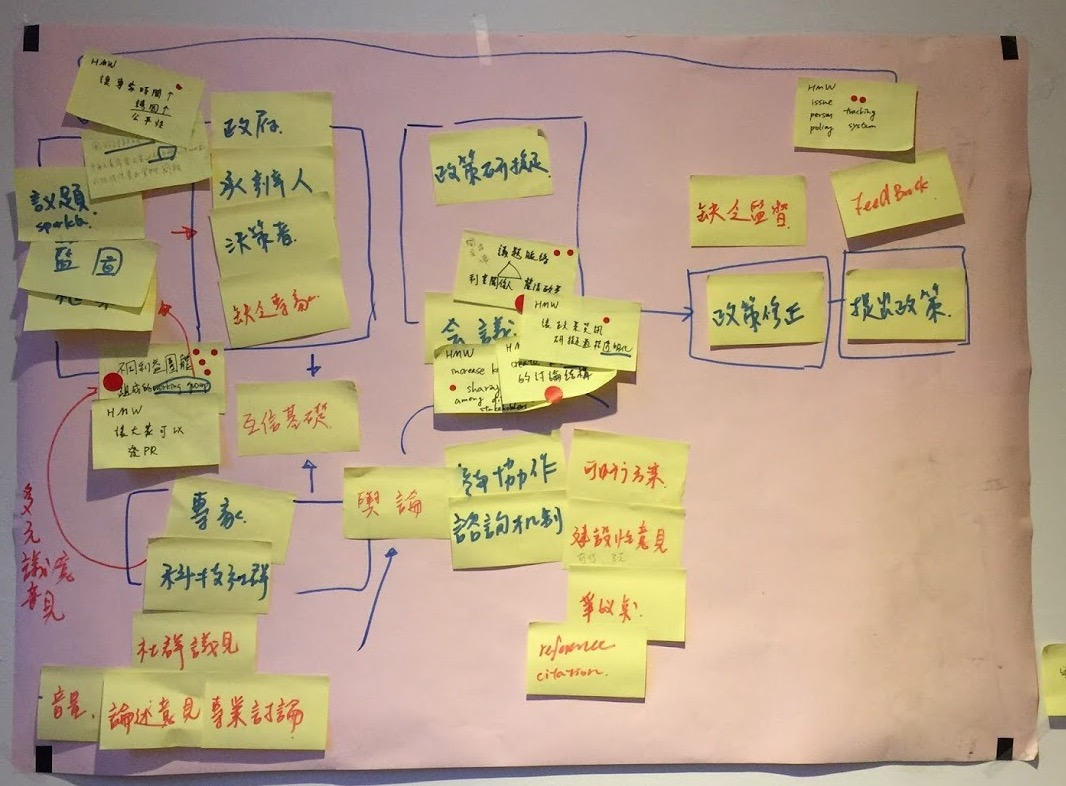
\includegraphics[width=.9\linewidth]{./images/design_sprint_map.jpg}
\caption{\label{fig:orgdf5af62}
Design Sprint Map——定義關鍵環節}
\end{figure}

最後選擇兩個關鍵環節:
\begin{enumerate}
\item 如何找到網路社群/專家作為利害關係人參與政府會議或網路意見收集
\item 如何幫助與會者語彙知識對齊、對議題脈絡有全局觀
\end{enumerate}

因研究資源限制,團隊選定專注在從公民、網路社群的角度,如何設計工具與機制讓網路社群能夠自組織產生論述的過程中對議題脈絡有全局觀、知識語彙對齊,讓產生出來的論述能被納入政府會議或網路意見收集過程之中。接下來使用服務藍圖、顧客旅程圖等分析方式,進一步挖掘目前網路社群參與公共事務討論的痛點,以開發解決工具與討論機制。
\subsection{服務藍圖}
\label{sec:org1cfda34}
透過服務藍圖透析社群團體在陳議議題時的工作流程、協作方式、議題擴散與跟關係人接觸互動的過程。從流程裡,了解目前社群團體在討論/倡議議題的時候,扮演關鍵影響的人(利害關係人)、事(會議、事件、擴散活動)與物(溝通、協作、擴散工具)間扮演的角色與其互動流程。

我們採用服務藍圖以系統性的方式將訪談倡議民眾/團體的倡議過程記錄下來,整理成清楚易懂的流程表,降低理解的門檻,讓站在倡議民眾立場外的人也能理解倡議民眾在活動過程中的旅程。另外,服務藍圖的鳥瞰視角,清楚的將「前台」( Front Stage)、「後台」( Back Stage )與「幕後」( Behind the Scenes )三個區塊的運作樣貌呈現出來。讓我們可以清楚地看到,在民眾倡議議題的過程步驟中,每一個階段背後採取的行動、使用的工具、參與的人員與相關的利害關係人,以這樣的架構釐清倡議民眾在執行倡議過程中的幕後準備行動,也能讓我們看到早期議題形成的發展脈絡。

\begin{figure}[htbp]
\centering
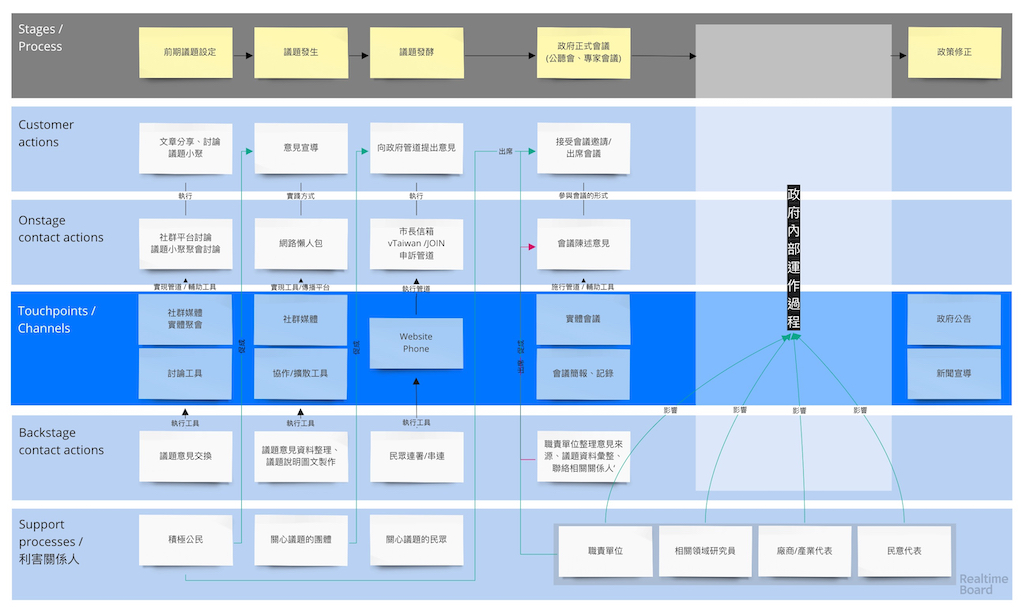
\includegraphics[width=.9\linewidth]{./images/service_blueprint.jpg}
\caption{\label{fig:org0418efb}
網路社群公民參與服務藍圖}
\end{figure}
\begin{enumerate}
\item 服務藍圖架構解說
\label{sec:org72d110d}
服務藍圖的架構雖有常被廣泛使用的模板架構,但隨著目標物、流程範圍、精度與目標對象的不同,在結構上會稍作調整以完整描述流程樣貌。

最上層是倡議議題的各個階段。將訪談者參與議題倡議的過程統整成概括性的經驗流程,也可以將上層階段視作倡議議題時經歷的流程步驟。

在一般的模板架構,會將流程中的 physical evidence 列在最上層,作為在每個步驟中影響顧客訊息接收的接觸點,如餐飲店的制服員工、自助點餐機台等物件,無論潛在或實際上傳送品牌意涵、實際訊息給顧客。但在民眾參與倡議的體驗過程中,並不會一致地接觸到相同的線下觸點,在流程中,最為重要的行為「溝通協調」經常發生在數位平台上。在多位受訪者的訪談資料中,我們看到數位工具除了擔任連結同議題的倡議民眾溝通協作的觸點要角之外,同時是連結前台行動與後台行動的「實行通道」。因此,在本設計案我們將 Touchpoint / Channels 層放在 Onstage 與 Backstage 階層的中間,以顯其作為實行通道的功能角色。

在議題倡議的每個階段,積極公民倡議的過程中都有相似的行動(Customer Actions),而每個行動慢慢的促成下一階段的發生。Onstage Comtact Actions 是倡議民眾每階段行動的實際動作(促成行動的實際行為);Backstage 則是每個實際動作背後的運作動作。例如,在意見宣導的行動階段,實現意見宣導的是藉由散播議題懶人包的方式讓更多人看到/看懂議題發聲的緣由,而懶人包的製作過程是一般人看倡議民眾倡議議題時看不到的後台行為。利害關係人,則是因為自己立場對議題有不同解讀與態度的人,會影響每個階段議題倡議行動方向、活動、宣傳內容定調等,像是決定議題懶人包切入論述的角度。

\item 參與途徑說明
\label{sec:orgba300a0}
本節說明 \ref{fig:service-blueprint} 各階段細節。
\begin{enumerate}
\item 前期議題設定:
\label{sec:org94f24cf}
在重大議題尚未發生之前,通常會有一群關心該議題的積極公民,因為工作/生活跟該議題相關,而關注討論該議題的發展。議題討論可能會鬆散的發生在社群平台,或是討論該議題的協作工具上。稍微有組織力的討論活動,則是發起線下的議題小聚討論會,透過線下群聚討論,並用數位工具紀錄討論過程。
\item 議題發酵:
\label{sec:org69aa47c}
議題可能因為前期討論而持續發熱,或者因為突發事件而使得議題開始被注目。在這個階段,積極公民乃至有組織性的議題團體會以自身立場對外界作意見宣導。宣導的方式有許多種類/途徑,常見的有文章、圖文解說、懶人包等。懶人包的製作需要透過數位工具的協作,像是討論解說文字的脈絡、引文查找、對應圖片繪製等等。而懶人包的傳播則經常是透過社群媒體擴散出去,常見的平台像是臉書、PTT、電子郵件、專屬網站。
\item 正式行動:
\label{sec:org1e25160}
正式行動階段是議題被大眾廣泛的討論與關注,人們開始重視這個議題。而議題在大眾的發聲之下進入政府內部系統,進入的管道可能是市政信箱、連署平台或是其他申訴管道。民眾串連、連署的媒介則是透過連署網站,有時也有民眾用灌爆單位信箱、電話的方式表達意見,讓職責單位意識到議題的重要性。
\item 政府正式會議:
\label{sec:orgac5cd6a}
當議題進入政府單位後,運作方式有很多種,但形式相似,都是以政府正式會議的方式集結眾人對該議題再次陳述其立場。召開議題會議前,相關職責單位會先行整理該議題相關資料,如研究文獻彙整、他國相似案例、查找議題相關的利害關係人、代表性專家學者。待內部先行了解議題狀態後,聯絡相關人員邀請參加會議。有時,因議題的急迫性,職責單位的準備時間而有所簡短,與會人員事前收到對於該議題的資料不一定俱全。有時準備出席會議的與會人會事先提供自己準備的資料,請責辦人員提供給會議上的其他人參考。會議會有會議記錄,紀錄會議上每個人的意見發言,但因與會人的立場紀錄不一定會公開。會議後的後續成效不得而知。
\item 政府內部運作過程:
\label{sec:org0f5e5c8}
經過前上述政府正式會議政府單位搜集各方意見後,了解各方利害關係人的立場與目前議題影響的範圍,或評估議題未來影響的程度,討論政府於該議題的態度方向、執行的動作、可用資源該如何應用。
\item 政策修正:
\label{sec:orgcc4f6fb}
經政府評估議題之影響,與政府目前可行之動作後,對該議題相關的政策作修正。
\end{enumerate}

\item 現有網路參與機制與本計劃定位
\label{sec:org0f1a343}
完成服務藍圖後以此檢視我國可供科技社群反應科技政策之常態性的中央政府網路參與機制,主要有數位經濟法規線上調適平台 vTaiwan 與公民政策網路參與平台 JOIN。

\begin{enumerate}
\item 數位經濟法規調適平台 vTaiwan
\end{enumerate}
vTaiwan(\url{https://vtaiwan.tw/})
由政府部會和民間提案,針對數位經濟相關法規做討論,共有五個階段:成案、意見徵集、研擬草案、送交院會、歷史案件,透過每週三線下社群小聚協助前期議題釐清與架設網路討論空間,如:共筆、提案介紹、直播、討論區、pol.is 收集意見,邀請參與諮詢會議的利害關係人,並召開線下諮詢會議搭配直播與網路留言。

\begin{enumerate}
\item 公民政策網路參與平台 JOIN
\end{enumerate}
公民政策網路參與平台 JOIN(\url{https://join.gov.tw}), 由行政院國家發展委員會建置,我國公民與在台外籍人士都可線上提案,經過檢核所提案事項為行政院職責範圍內及通過其他標準,即開放附議,提案若在 60 日內在 JOIN 平臺上附議超過五千人,主管機關需在二個月內於該平台上正式回應提案。

\begin{figure}[htbp]
\centering
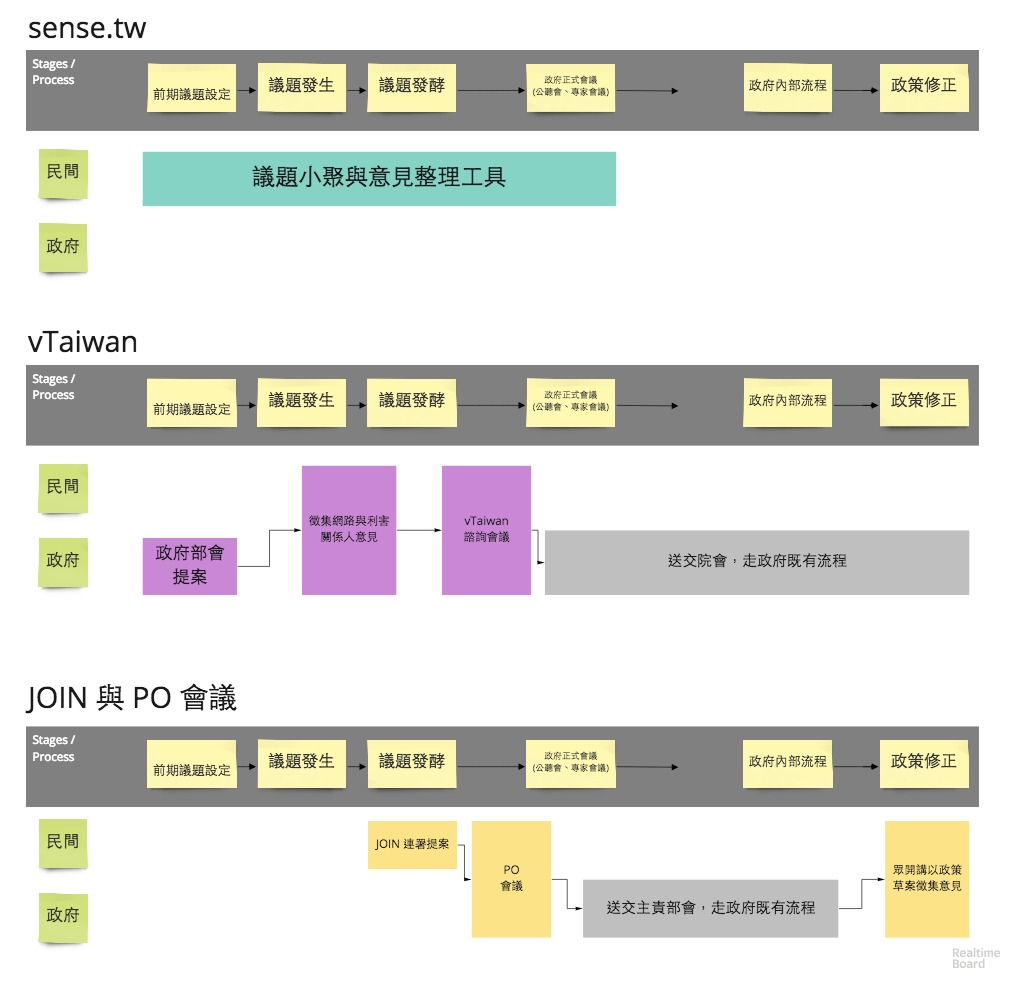
\includegraphics[width=.9\linewidth]{./images/sense_vTaiwan_JOIN_diff.jpg}
\caption{\label{fig:orgbe76d4e}
網路參與機制在服務藍圖上之定位}
\end{figure}

由 \ref{fig:sense_vTaiwan_JOIN_diff} 可見 vTaiwan 和 JOIN 主要是在政府端處理非正式的諮詢會議和會議前的議題釐清。

vTaiwan 實際上由政府部會發動議題設定(二十幾案中只有一案為民間提案)\footnote{截至 2018 年 11 月 5 日為止,成案二十幾件案件中,只有「違反本人意願而散布本人的身體私密影像」一案為民間提案,成案網址:\url{https://vtaiwan.tw/topic/nonconsensual-pornography/}。},在議題發酵階段與網路社群討論,在進入政府正式會議(如公聽會、專家會議)之前,有線上線下整合的諮詢會議,其會議結論無剛性要求主責部會執行,可視為與社群討論的會前會。

JOIN 平臺則是扮演了接收民眾陳情和提案的窗口,雖有「協作討論區」讓正式提案前即可徵求網路意見做修改,但基本上不處理前期民間的議題釐清。JOIN 在連署成案的案子,部分會經由行政院內開放政府聯絡人會議(Participation Officer Network)\citep*{lin17} ,召開開放政府協作會議進行議題釐清與多方利害關係人會議 ,使用直播、數位白板等線上工具公開會議流程,政策修正則會放在同一網站之眾開講之部分,收取線上政策回饋。

本計劃(sense.tw)定位則是為前期協助網路社群做民間議題釐清,以促成社群有正式行動,進而參與政府會議,並不處理議題和政策進入政府內部後之流程。其設計是為了讓進入正式提案的點子可以更好,而非再架設一個新的網路參與機制平台。
\end{enumerate}
\subsection{顧客旅程圖 }
\label{sec:org64c6ed3}
顧客旅程圖是一種從服務藍圖中衍生出來的圖。兩者在架構上相似(照前後順序排列的結構),但在觀點、範圍、聚焦和使用上多少有所相異。\cite{james2017} 服務設計藍圖主要用於描繪整體環境,先歸結主要的議題倡議步驟階段、重要行動、利害關係人互動形式。接著再用顧客旅程圖將倡議民眾每個執行動作(與執行該動作的接觸媒介:數位工具)盤點出來。顧個旅程圖不僅只是盤點觸點的工具,它包含的元素除了觸點外,亦包涵了「行動」、「情緒」、「目標」、「關鍵時刻」、「痛點」、「機會點」等。本設計案藉由 CJM 工具,找出倡議民眾倡議行動中遇到的問題點,並找出協助議題釐清的數位工具在倡議過程中能提供協助的利基點。
\begin{figure}[htbp]
\centering
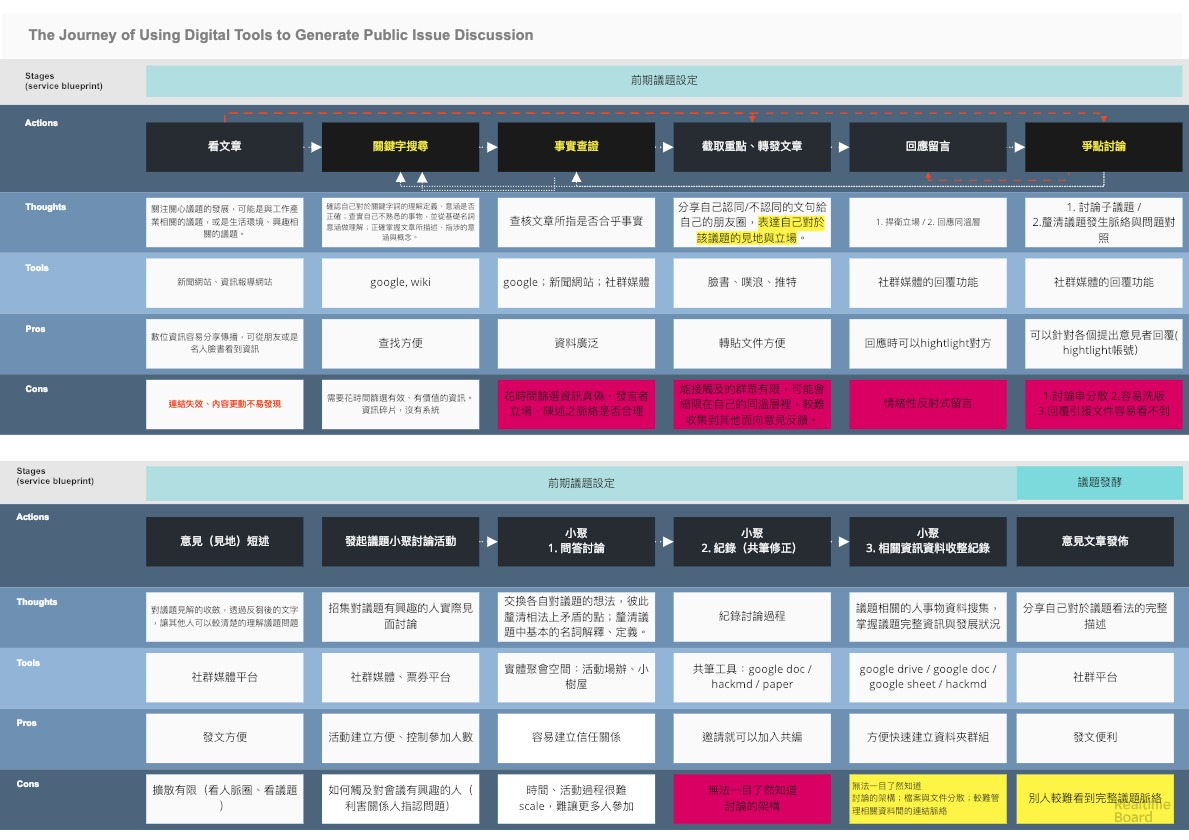
\includegraphics[width=.9\linewidth]{./images/cmj1.jpg}
\caption{\label{fig:org873818b}
顧客旅程圖}
\end{figure}

這張旅程圖仍沿用前面服務藍圖的前四個階段(Stages):「前期議題設定」、「議題發酵」、「正式行動」、「政府正式會議」。以四大階段作為行動目標的主架構,底下詳細紀錄在個階段執行的動作,含括服務藍圖裡的前台動作與後台動作。四個階段 (stage)可以視作為動作 (Actions) 執行的時機點「when」。Thoughts 探討每個「action」背後的目的與需求,有助於我們除了看到「 What - 什麼動作被執行」,也能看到「 Why - 為何採取這個行動」,協助我們辨識積極公民在倡議過程中的關鍵步驟以及積極公民與一般民眾間的差異點,找到設計上能切入提供協助的缺口。「Tool」是指執行每個動作時使用的工具,亦即「How - 動作是如何被執行/實現」。除了列出使用的工具外,藉由列出工具使用的優缺點 (pros and cons)找出目前流程上可以協助改進的痛點 (pain point) 。倡議民眾在議題倡議的過程中目標對象主要是「大眾」與「政府」,通常前期階段的溝通對象為大眾,目的在於讓更多人了解議題。後半階段的溝通對象則是政府與相關利害關係人,政府與相關利害關係人才能對議題政策修正有影嚮力的決定。
\begin{enumerate}
\item 前期議題設定
\label{sec:org463fc97}
這個階段描述倡議民眾「了解議題」、「形成觀點」與「議題社群的形成」過程。倡議民眾因為自己的生活環境、工作、興趣等因素,對議題產生關注,關心議題的發展。平時會在新聞平台、社群平台看議題相關文章、新聞。在閱讀的過程對文章中不了解或有疑義的部分會進一步搜尋相關資訊,透過關鍵字搜尋,查找網路上相關資料。累積一定程度對議題的了解,加上自身經驗,建立自己對於議題的觀點。過程中,看到激起共鳴的文章會截取重點、轉發到自己的社交平台上,表達自己對於該議題的的立場與想法,讓自己的朋友圈能一起注重該議題。轉發文章、發表自己的意見有機會能促發網路上的朋友、民眾在發文底下留言,交換意見。在目前的社群平台上,經常看到針對某一議題,因為民眾對該議題的認識深度不夠深,在全面了解之前,看到文章或發文可能所含的特定觀點立場,就陷入情緒反射式留言,而非了解該意見所處之立場。「事實查證」、「爭點討論」是議題倡議積極公民與一般大眾最大差別的地方。議題倡議的積極公民具有獨立思辨能力,有能力辨識資訊真偽不被混淆,並有能力理性思考其他意見的立場成因,找出議題爭點背後矛盾拉鋸的因素。

小聚活動是了解議題的人或是對議題有共同討論點的人發起線下群聚討論的活動,夠過線下聚會、面對面交流,有助於彼此在議題上的意見交換,也更能建立信任關係,讓議題討論的深度加深,廣度更全面。由於議題的複雜度、牽涉的層面廣度以及與會人的自身立場,會讓小聚開始時較難聚焦、釐清彼此意見的脈絡。也需要花時間做議題相關之名詞定義,好讓參與小聚的人的認知調校到相同的刻度上。清楚的議題脈絡架構能協助議題討論的人快速同步對於議題的基礎知識,也能提升討論的品質。

成型的討論群組聚集了很多議題的資訊資料,除了每次小聚討論的紀錄,還有各個成員分享的與議題相關的參考資料。這些資料幫助群組內的成員對於議題了解的深度,但些資料累積到一定量後,很難整理,也很難讓新加入的人有系統、有脈絡的了解這些資訊,增加了新加入討論的人的門檻。

\item 議題發酵
\label{sec:org0783720}
議題的發酵一般來說都與某一事件發生有關,大眾對該事件的關注使得背後的議題被看見。倡議民眾與議題發酵階段才開始注意議題的民眾不同,他們在先前對議題的脈絡、成因、問題已有相當深度的了解,並有一套自己的觀點。 在議題發酵階段,倡議民眾或相關的倡議團體致力於讓一般大眾能了解議題的問題,讓更多人關心這個議題。他們會在社群平台、媒體投書、短講這類發聲平台,講述自己對議題的看法,希望能影響更多的人了解、同意、支持他們的立場與意見。為了要讓更多人理解與認同,倡議民眾除了發表自己的看法之外,也會觀察大眾對該議題的意見、對議題的疑義。透過回覆解釋一般民眾對議題的疑義誤解,引導民眾看到更深的層面,並希望從而獲得認同。

我們以製作懶人包作為倡議民眾議題擴散於其他民眾的範例,懶人包較於其他文字擴散形式多了說明圖文的製作步驟,但整體的發想、整理流程與其他擴散媒材的準備過程大致相似。懶人包的製作通常是多人線上合作完成,群體內部需要先對議題的認知與意見方向有共同的基礎,線上協作的過程也需要一套團體內部方便協作的工作流程。但是即使有相同的意見基礎、協作模式,線上協作文件條列片段式的資料整理形式仍增加協作上溝通成本,這樣的文件形式較難表現議題子脈絡間的關聯。

議題發酵是倡議民眾、倡議團體與大眾溝通並擴散議題的階段。以有根據支持的精煉過的意見陳述,影響更多民眾對議題的關注與支持;為了能夠說服更多民眾,所以去理解其他民眾對議題上的提問與意見,並找出相關支持的事實與文獻與之回應以獲得支持。這是一個滾動的過程,在滾動來回對話的過程能夠讓議題擴散得更遠,觸及更多不曾接觸到該議題的人,並為他們對議題建立最初步的認知。更多的人支持倡議民眾/團體的意見方向,公眾的聲量與影響力促成倡議民眾/團體進入下一個階段。
\item 正式行動
\label{sec:org096bc67}
正式行動階段是串連意見相同的公眾力量,讓這股力量被政府看見,並將陳情傳達進政府管道,使政府內部關注並處理該議題。這個階段一開始仍是藉由各個媒體社群平台將連署串連的行動推廣出去,為了要在短時間引起民眾的共鳴,這個階段說明的文字通常會較之前的階段更簡短。雖然訴求簡潔有力能快速引起共鳴,但這個階段的發文較難完整的交代議題所有脈絡,使得接觸到串連宣導的人較難完整的理解議題全貌。

除了吸引其他民眾理解串連的意義外,這階段倡議民眾/團體的重心放在如何使串連的人數增加,如何讓集中起來的聲量讓政府看到。倡議民眾/團提在這個階段除了持續更新議題相關資訊、擴散議題意見外,部分時間與心力則是放在引導大眾如何進行連署,藉由朋友圈間相互引導串連,讓議題通過連署門檻。
\item 政府正式會議
\label{sec:org79971cc}
當民眾的陳情意見進入政府內部後,相關職責單位便會著手規劃舉辦議題相關會議。相關職責單位內部也有一套自己的研究調查流程,研究該議題的脈絡、問題點、影響範圍、利害關係人、衝突點等因素。找出各面向的利害關係人代表後,邀請這些議題相關人士(專家、學者、倡議團體、代議士、企業代表等)參與會議。本計劃訪談到的倡議民眾大多表示在參加政府相關會議前都會事前準備議題相關資料,希望參與會議的人能先了解自己對於議題的主張與見解,但大多時候在參與會議前無法事先知道與會的其他人以及他們對議題的看法。訪談對象表示,這樣讓政府相關議題會議變成與會人在會場上發表各自對議題的看法,彼此的對話沒有交集,因此很難在會議上對議題討論出共識。訪談對象共同指出,目前的政府會議流程缺少了事前讓與會人彼此核對議題認知、補平知識落差的流程。各自對議題名詞解釋、議題脈絡的認知有落差,使得彼此意見、溝通對談的話語難有交集。

除了會議前缺少知識語彙對齊的環節,會議後參與會議的倡議民眾也遇到無法收到會議後續回饋的問題。政府單位的會議記錄與議題討論不像開源團體或是倡議團體採用開放協作模式,讓參與的人可以一起記錄會議,另外,大部分會議礙於無法公開會議過程也無法公開會議記錄。這使得會議的後續反饋變得很少,與會的倡議民眾也無法得知自己參與相關會議對於政府對該議題的政策規劃是否有實質的意義。同樣的,外界民眾也很難理解這些會議的實質影響與效益。
\item 整體問題發現
\label{sec:org026a639}
整個旅程雖然分成四個階段,但我們發現數位工具用於議題資訊整理貫串在各個階段,不同立場的各個單位(倡議民眾、倡議團體、政府職責單位、相關利害關係人)都需要透過數位工具整理議題資訊,如:新聞剪報、文獻節錄、人事物時間表。這些議題資訊整理的文件每個階段至少都會製作一份(或是一個版本),但這份文件卻很難串接延續到下一個階段,在整理與精簡化的過程,這些搜集來的資訊與原本的來源失去鏈結,片段資訊彼此之間的脈絡也變得不明顯。

另一方面,在議題討論的溝通過程中,不論是實體討論或是線上協作討論,基礎階段都需要經過核對議題相關的名詞定義、議題問題理解、議題脈絡、議題範圍等認知與知識語彙對齊的階段,這些資訊的來源最好是來自相關研究文獻、報告、書籍等具可信度的文字來源。有些議題團體在整理資料的過程會把重要基本資訊存成 PDF 檔案,放在雲端儲存空間,但同樣有在檢視資料時,追朔回原文獻困難、連結斷落的問題,另一放面來說,這樣的協作模式增加了新進人員的檢閱協作的門檻。

訪談倡議民眾、倡議社群與 PDIS 協作會議籌備人員關於如何促進議題討論,我們總結出「以視覺化方式開展議題脈絡」能讓處在不同意見層面的人們能找到對話基礎的促進方式。無論是在線上討論或是實體討論,在討論的過程中,最重要的基礎步驟便是彌平參與討論的人對議題認知上的落差。議題脈絡圖是一個能夠讓人理解自己意見再議題背景中所處的立場位置的工具。除了理解自身立場之外,同時能擴充對於議題的認知面向,有助於參與討論的人將思考的範圍層面拉大,用宏觀的視角去思考議題問題,也較能以同理的方式理解對立意見的立場。此外,脈絡圖的圖面上需要能夠指出各脈絡間的連結關係,才能讓人掌握議題的成因、問題、目前解決方案、解決方案的影響等關係狀態。

觀察整體顧客旅程圖,可以看到每個階段不同立場的倡議民眾/團體都會做資料整理的籌備動作,最後政府會議的籌備單位也會對議題做資料研究。但是會發現這些議題資料整理完後無法有效的串接到下一個階段,或是無法擴散出去作為其他人對議題探討的基礎,更無法讓相關與會的人事前交換議題資訊。

每個行動的需求點,目前都有可對應的數位工具完成需求任務,但我們發現目前這些數位工具的功能仍無法協助銜接下一個倡議階段的發展。綜觀上述的問題發現與需求描述,我們認為目前協助議題倡議的數位工具至少要具備如非同步協作、文獻來源回溯、視覺化議題脈絡g、脈絡關係描述、資訊種類描述等功能。具備上述功能的數位工具,能讓議題資料整理以脈絡化的的方式呈現,同時能連結回原始文獻有助於評估資料可信度,並用視覺化的方式描述議題脈絡間的關係(問題點)。這種議題彙整工具可以促進剛接觸議題的人看到議題多元的面向,為議題理解的認知奠基,亦可以快速協助參與討論、會議的人在事前認識議題基礎知識,並促進討論/會議的討論過程。

除了相對應的數位工具,參與討論的人如何聚集和使用何種討論方法亦會影響其論述產出。在注意數位工具的同時,也需注意如何建立參與意願和使用數位工具之討論方法與品質。能夠聚集討論亦是使用數位工具之前提,故如何使網路社群有線上參與之誘因與自組織實質討論是開發機制之重點。
\end{enumerate}

\subsection{民間與政府溝通落差}
\label{sec:orgc55b9c1}
\begin{figure}[htbp]
\centering
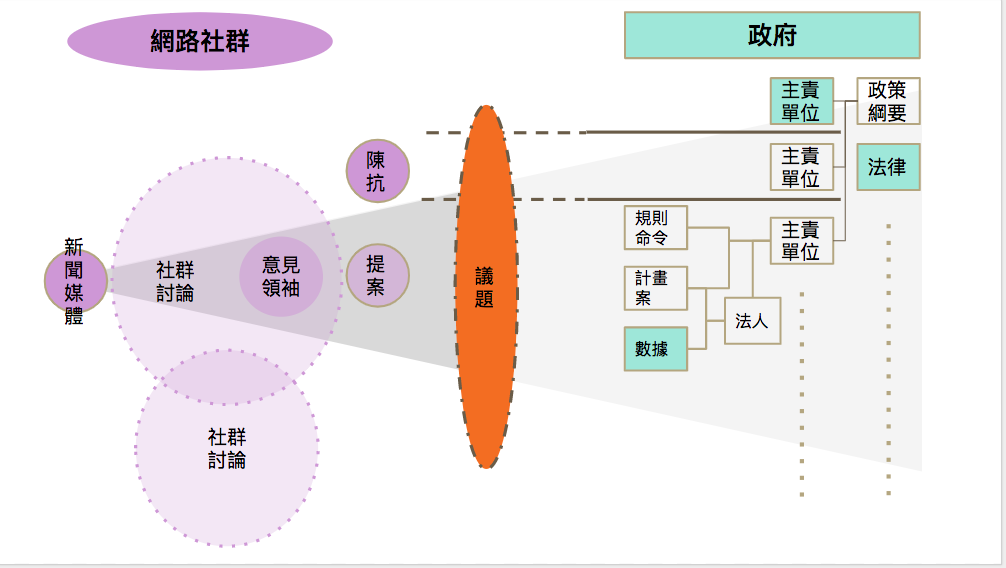
\includegraphics[width=.9\linewidth]{./images/gap1.png}
\caption{\label{fig:org36b78ad}
網路社群與政府溝通落差視閾圖}
\end{figure}

在開發數位工具與進一步訪談時,發現政府與網路社群的關鍵溝通落差,來自於視角不同。如 \ref{fig:gap1} 所示,民間網路社群是以議題、單篇新聞作為出發點批評政府,難以得知政策全盤規劃,報導也缺乏連結至原始政策文獻的方法,使網路社群在無法查證之狀況下,難以信任該政策規劃。舉例來說網路批評者批評為了發展 AI 購置多台超級電腦,但不知道同時間政府其他 AI 相關計畫;面對跨領域議題,例如 AI 人才培育議題,民間不會去區分是科技部、教育部還是經濟部主責,而是將政府視為一個整體批評。

然而,政府卻是以主責部會角度看待政策規劃,將政策切為不同部分讓部會主責,因此難以與民間對話。同時,政府在蒐集輿情時,多著重在主流媒體報導與陳亢事件,缺乏網路社群第一手資訊,想要尋找網路意見領袖進來開會即可,卻忽略網路上沒有代表人,而是有很多不同的社群在做討論,意見領袖只能作為與網路社群溝通的窗口,而不若傳統公協會之代表人。政府在收集網路社群意見時,遇到另一個困難是,網路討論碎片化又非常繁雜,不知道去哪裡找到洞見,既有輿情工具也只能做到網路關鍵字聲量分析,卻無法歸納總結爭點論述。

因此,希望能有數位工具和討論機制讓政府與民間的知識語彙可以對齊,才能推進相關討論 \ref{fig:grounding} 。民間因熟悉網路討論內容與空間,能先自行整理問題與訴求,政府則能提供完整政策規劃之原始資料與整體政策。

\begin{figure}[htbp]
\centering
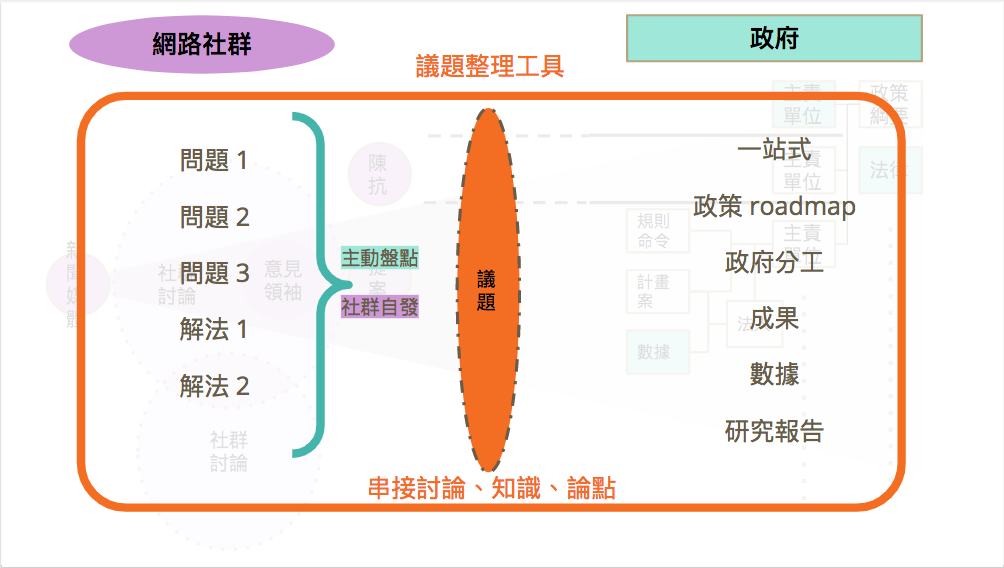
\includegraphics[width=.9\linewidth]{./images/gap2.png}
\caption{\label{fig:orgf1b9e5e}
建立知識語彙對齊之基礎(Grounding)}
\end{figure}

本計劃著重在銜接民間討論至政策規劃,目標在促進民間自組織釐清議題、了解政策後能提供政府洞見與訴求,因而開發
\begin{enumerate}
\item 數位工具原型開發做議題整理
\item 線下討論促進網路社群參與政策討論
\item 數位原民參與手冊供網路社群理解政策形成機制與公民參與方法\footnote{主要與現為軟體工程師的樹黨發起人討論。 樹黨發起人之目的為倡議 Public Money Public Code,撰有〈二十年後的政府軟體〉一文 \url{http://treesparty.tw/2018/06/17/public-money-public-code/}。\label{org2853c6b}}
\end{enumerate}

\section{線上線下整合的網路參與機制設計 }
\label{sec:org23e74d6}

由上一章之針對網路社群的公民參與服務藍圖與顧客旅程圖分析,可得知網路社群缺乏在前期議題設定、議題發酵階段能有適合的議題釐清的工具與線上線下串接的討論機制,並且需要工具做到溝通落差的視閾融合。

本研究希望嘗試在公民參與服務藍圖上的前期議題設定、議題發酵階段,能有線上線下的整合機制,讓網路社群可以自組織做議題釐清和知識語彙對齊,弭平溝通落差,進而促進討論品質。網路社群雖因共同興趣在線上集結,但線下活動亦是非常重要創造社群連結與討論的場域,故討論不只著重在線上,而是需要線上線下滾動式串接討論,目標讓對科技政策的討論低參與門檻、高頻、持續、多元,對接政策提案。 線上線下的兩種機制也可以分別實行,或與其他機制混合使用。以下章節分四部分討論:

\begin{enumerate}
\item 期望討論流程
\item 線上意見整理工具
\item 線下議題小聚
\item 線上線下整合串接案例
\end{enumerate}

\subsection{期望討論流程}
\label{sec:orge6c14c8}
「社交工具移除了公開表達意見的舊有障礙,也打破了大眾媒體的高進入門檻。其結果就是以往媒體專業人士所專有的權利已經交到了業餘公眾的手上」\citep*[p.59]{xue11_xiang},大規模的業餘化早已打亂了專業類別,人人都可發表論述並成為「受眾(audience)」\citep*{wimmer03_da} 所認定的專家。自媒體雖然成為了「異議者 」突破大眾媒體壟斷資訊傳播途徑之一,但也造成假新聞與極端言論的溫床。在這個「後真實(post-truth politics)」\citep*{wiki:posttruth} 時代,認定專業權威性(authority)的角色已從機構回到「受眾 」手上。我們希望公民對於公共議題的知情討論(informed discussion),來自於彼此貢獻知識與自主查證,而不必然需要專家告知或製作議題手冊,因為專家除了主觀意識造成的知識盲點外,議題也容易遭到「政客,媒體,政治顧問透過分析、界定、區格與標籤等手段將問題轉化成對社會真實的爭辯」\citep*[p.123]{yanyuan09_gong},為了用來混肴公眾追求仕途的工具進行與論操弄。任何專家告知其實已經隱含了一種「議題設定(Agenda Setting)」\citep*{wimmer03_da} ,然而往往「議題設定」卻是最需要被質疑的,爭執到最後才會發現誰才是議題專家或是發現告知者沒有揭露會造成判斷轉變的關鍵資訊,網路社群的意見領袖的權威性並非來自於頭銜,而應當來自其論述與提供的佐證資料讓他人可查證。

因此期望這個討論流程是鬆散的,讓下班後的公民可輕度持續討論 \citep*{xueji11_xia} ,不必馬上有結論,而是每個參與者皆可以以自己的方式再利用其討論結果,透過群眾協作收集議題之問題面向與可能解法,在不斷的迭代(iteration)循環討論中,自我修正與辯證,提升參與者之反思程度 \cite{fleck10} ,以加深討論深度以達到議題釐清爭點與凝聚社群共識之目的。從使用者訪談中,發現列出問題與回答的 QA 法普遍被倡議者和積極公民使用,易於網路討論和擴散。在此基礎上,新的討論流程的設計是在網路社群熟悉的討論空間以其熟悉的文化,例如要求原始資料連結、開放協作等方式,做到根基於佐證資料來源(source-based)地釐清問題(problem)、解法(solution)、論點(statement),對齊知識語彙(definition)、界定利害關係人(stakeholder),並且串連出來參與的積極公民(active citizen),讓他們互相連結(networking),導引到現有公民參與機制發起行動。

在問題界定跟知識跟語彙對齊期望發揮到是讓參與者問出「問題背後的問題」、「問題裡面的問題」、「解法裡面的問題」,以及「佐證資料在哪裡」、「大家對名詞的理解都一樣嗎」?此外透過問問題的深度,提升一個人對於概念的理解程度,並且透過與他人對話,隨時自我省視修正自己原有之觀點。不管是線下聚會討論還是線上討論,透過互相論證進行議題裡面的問題,可能解法跟名詞界定,盤出相關利害關係人、相關資訊,以達到以下目的:

\begin{enumerate}
\item 釐清不同領域的名詞(Ground Term)
\item 問出更深度問題(QBQ)
\item 頻繁而低成本的討論 (Micro Activity)
\item 跨時間地域的線上空間 (cyber space)
\end{enumerate}

由以上四個要點,讓每個公民可以貢獻其知識,做到彼此知識語彙對齊,透過辯證的方式回應建構論證,建立一般人也能輕度參與政策討論,並且有討論品質,等於是用數位工具擴展第四代政策回應建構評估(Responsive Constructive Evaluation) \citep{guba01} 模型,讓不只是專家和政府找的利害關係人去回應建構評估一個政策,而是任何公民與網路社群參與者皆可發動並參與這個過程。

\begin{figure}[htbp]
\centering
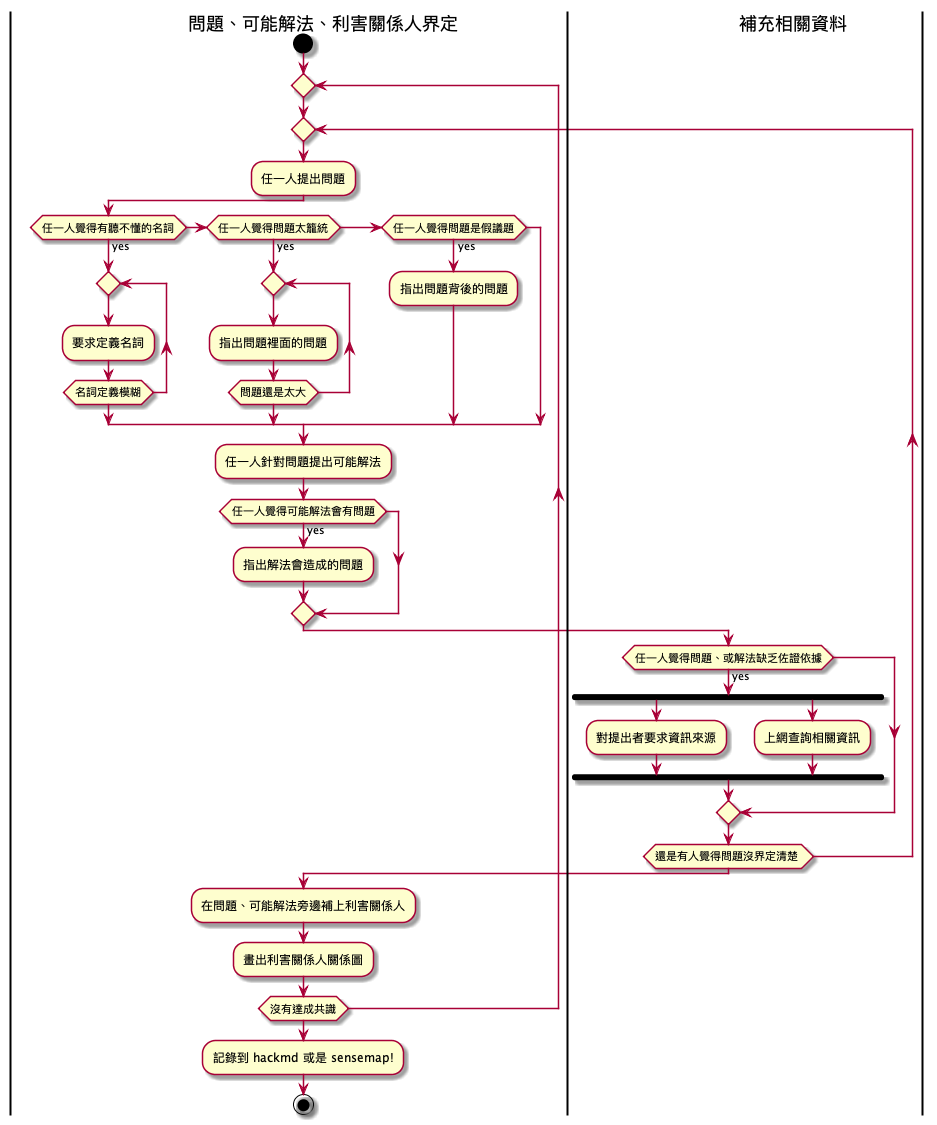
\includegraphics[width=.9\linewidth]{./images/problem_idenity_flow.png}
\caption{\label{fig:org9e367c3}
期望討論流程}
\end{figure}
\subsection{線上意見整理工具 sense.tw }
\label{sec:orgff11195}
在知識語彙對齊來提升網路討論品質的前提下,數位工具的開發希望能協助網路社群在前期議題設定的議題釐清階段,引入上述期望討論過程,並且工具設計著重在以下兩點:
\begin{enumerate}
\item 回歸原始資料來源
\item 呈現議題脈絡
\end{enumerate}

此意見整理工具 sense.tw 在敏捷迭代式開發下,經過三個 prototype,兩版產品改版,最終做出可在原始文獻上標記摘要,並以概念圖(concept map)、心智圖(mind map)、論證圖(argument map)等方式組織原始資料與論述的意見整理工具。

使用者測試曾分四種人物誌 — 積極公民(active citizen)、會議催化者(facilitator)、政策分析師、政務官—作為測試,發現使用族群須為喜歡嘗試使用新數位工具的人,並不依照身份別劃分,最終依工具使用情境定位在
\begin{enumerate}
\item 個人整理大量資訊
\item 線上非同步協作
\item 現場會議之數位記錄
\end{enumerate}

搭配線下線下之議題小聚討論,針對網路社群做推廣,尤其是需要在社群中凝聚共識與釐清爭點與政府溝通的網路社群參與者。
\begin{enumerate}
\item 工具使用情境與功能介紹:
\label{sec:org37794ba}
以下以個人整理大量資訊的情境作為工具功能介紹,線上非同步協作和現場會議之數位記錄會於線上線下串接案例中介紹。
\begin{enumerate}
\item 個人整理大量資訊
\label{sec:org882cba4}
在此以整理 2018 年底「以核養綠」公投論辯為例作為工具介紹。當時有兩場電視辯論會針對「公投第十六案:您是否同意:廢除電業法第95條第1項,即廢除『核能發電設備應於中華民國一百十四年以前,全部停止運轉』之條文?」做正反方論辯,有網路直播並且有辯論逐字稿,然而核能議題複雜也需要非常多佐證資料,故以此作為案例整理論辯架構圖,並連結回原始連結,完成如下圖的分析圖,在網頁上可放大縮小檢視。

\begin{figure}[htbp]
\centering
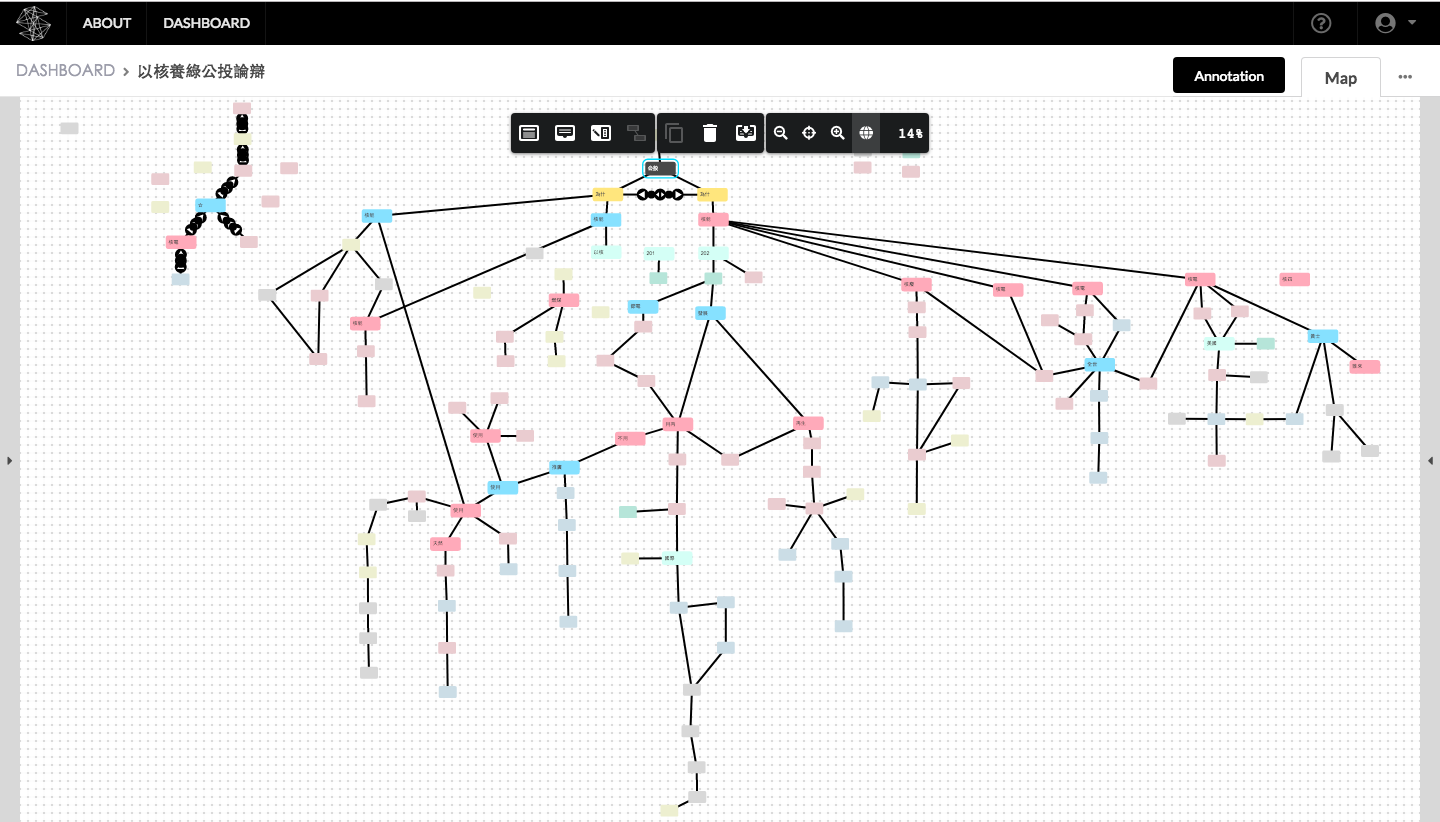
\includegraphics[width=.9\linewidth]{./images/nuclear_whole_picture.png}
\caption{\label{fig:orgf95bf1f}
以核養綠電視論辯分析圖全局觀}
\end{figure}
\begin{enumerate}
\item 在原始網頁、pdf 上註解。
\label{sec:org4faaf48}
sense.tw 可直接在網頁和 pdf 文件上畫重點註記。在此案例中使用此功能註記 HackMD 共筆上之辯論逐字稿,將單一論點論述與單一資料拆開紀錄,並且標上發言者與重點摘要,如下圖。

\begin{center}
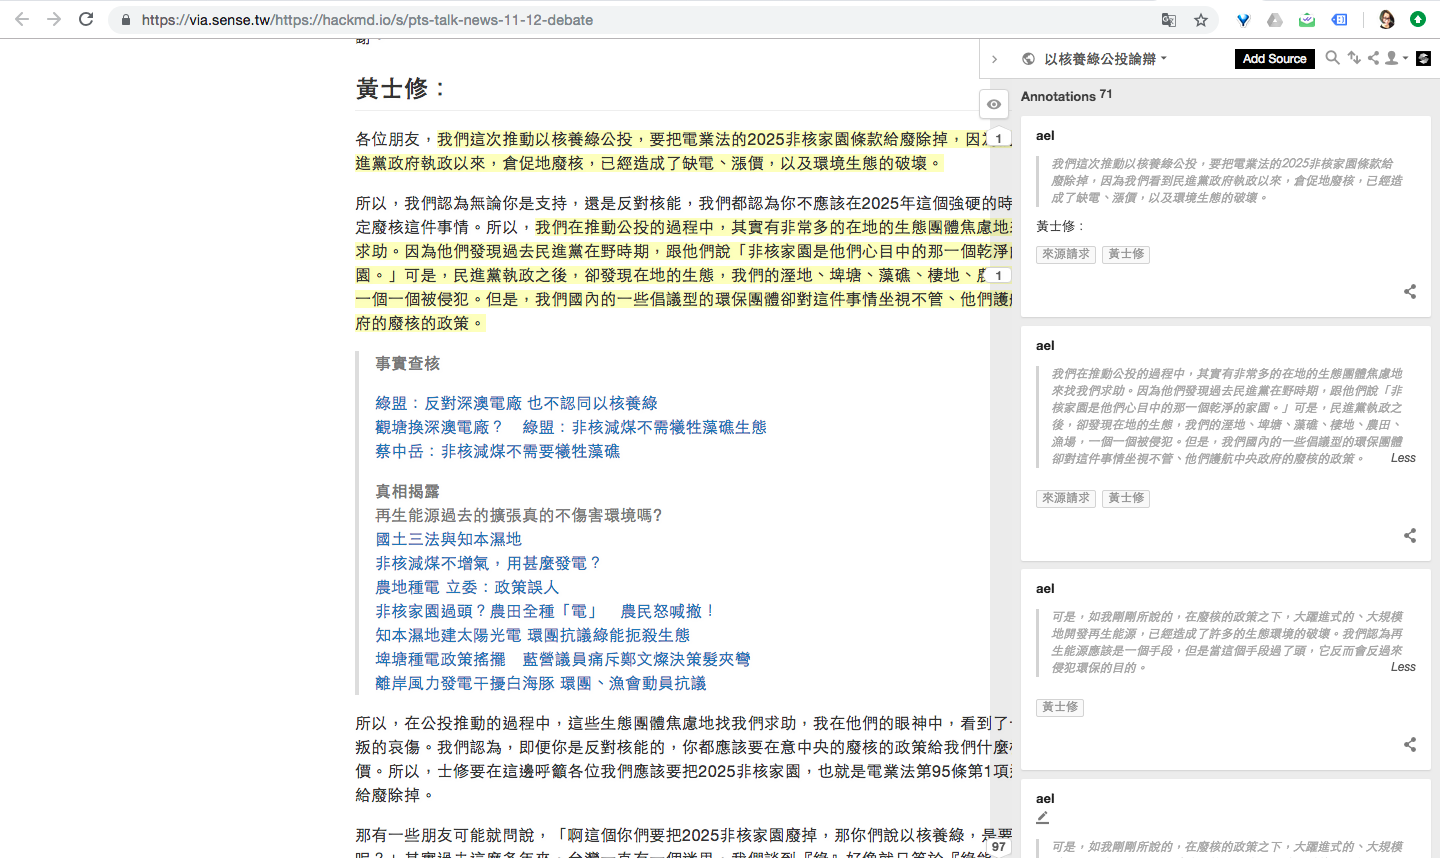
\includegraphics[width=.9\linewidth]{./images/nuclear_annotation_hackmd.png}
\end{center}

也使用此功能註記 IPCC 文件作為補充資料,如下圖。

\begin{center}
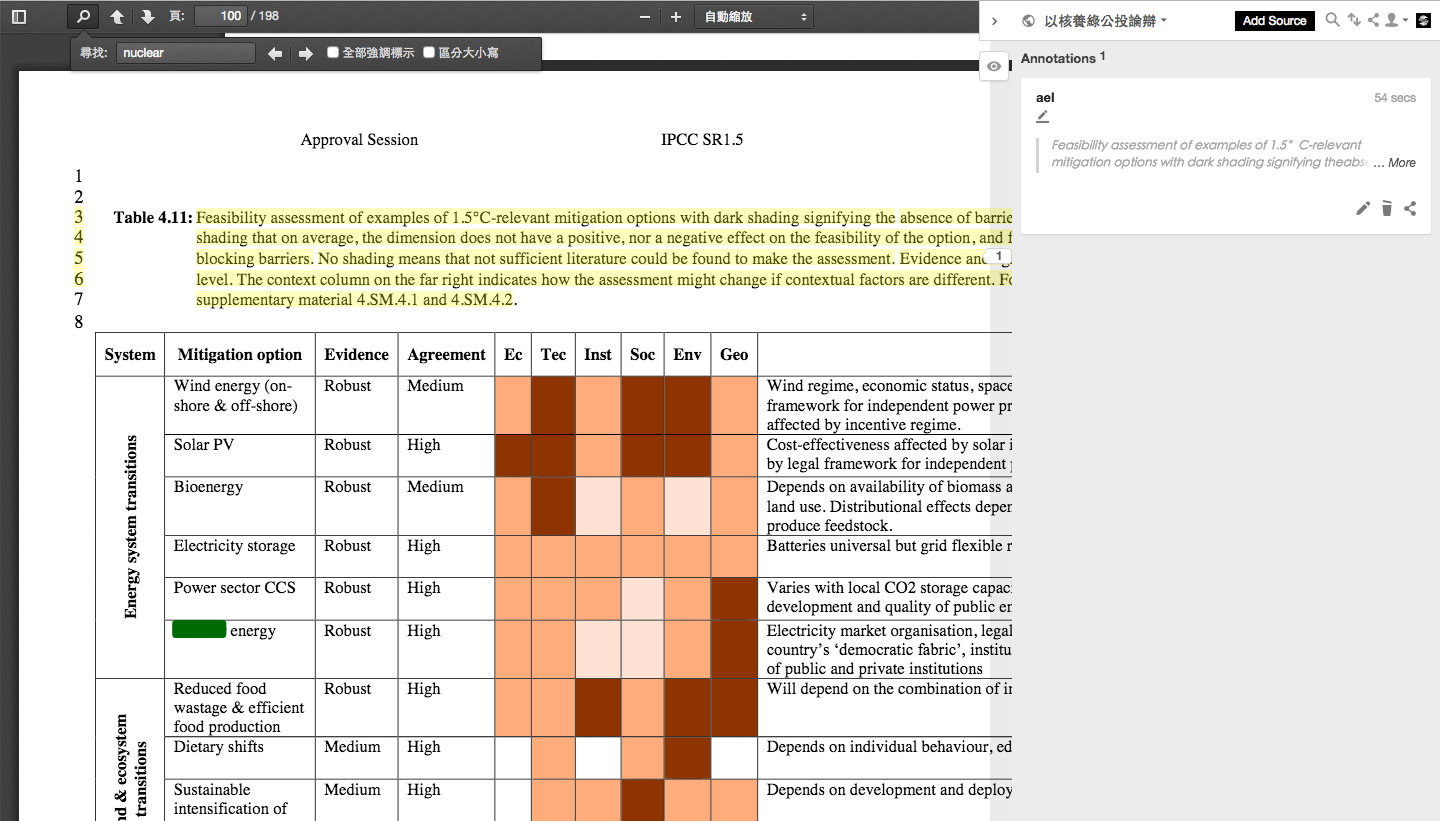
\includegraphics[width=.9\linewidth]{./images/nuclear_annotation_pdf.png}
\end{center}
\item Map Editor:群組、分類、連線、回應
\label{sec:org334cda8}
所摘要的註記,可在 Map Editor 介面作為 Card 被編輯,並可加入更多敘述、標籤、相關利害關係人。

\begin{center}
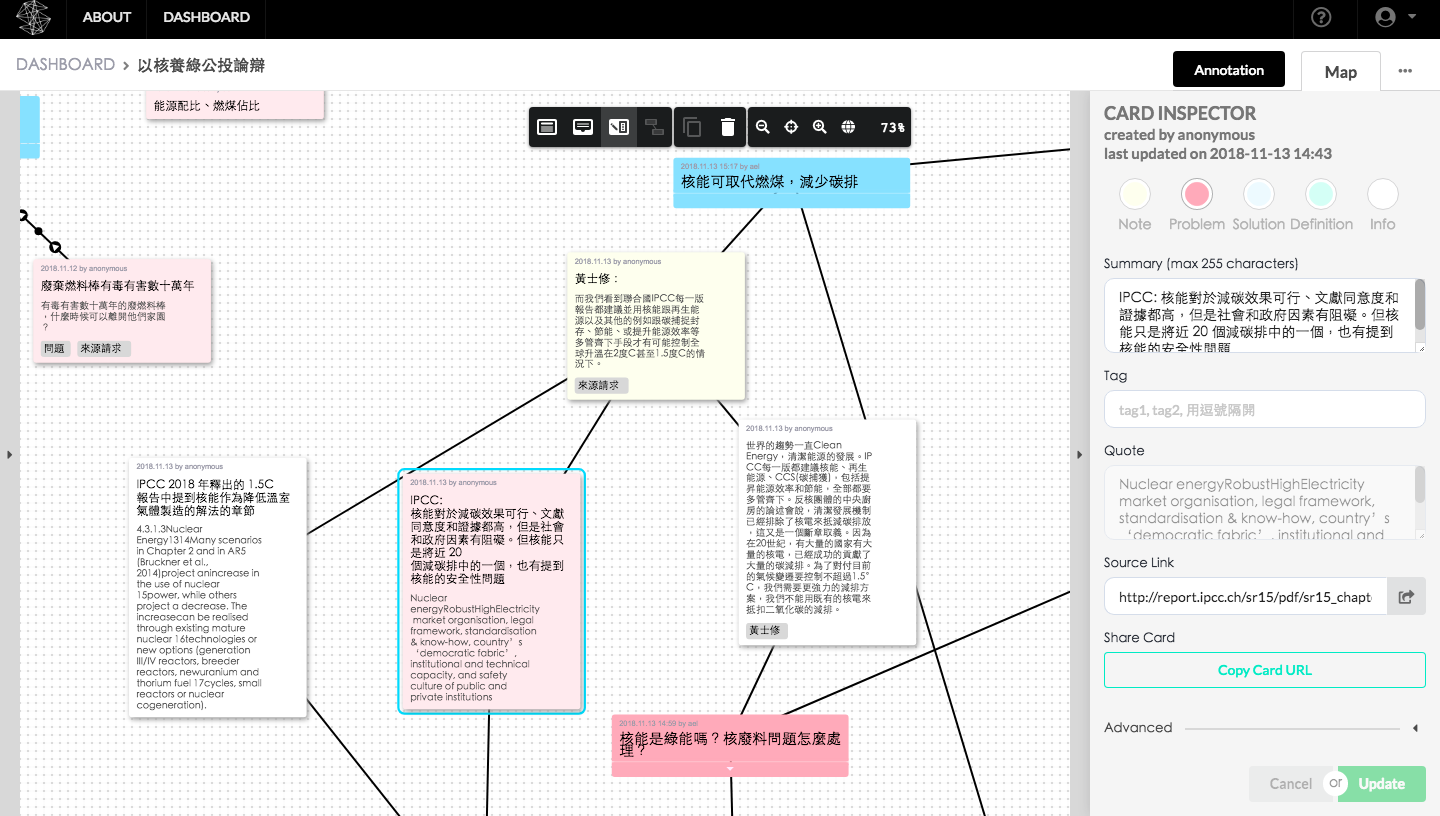
\includegraphics[width=.9\linewidth]{./images/nuclear_inspector2.png}
\end{center}


也可以單獨在 Map Editor 創建 Card,Card 有五種種類分別為不同顏色,以引導網路討論與分析:
\begin{itemize}
\item 紅色:問題(Question)
\item 藍色:回答(Solution)
\item 綠色:名詞定義(Definition)
\item 黑/白色:補充資料(Info)
\item 黃色:意見(Note)
\end{itemize}

另外,可看到較長的長方形為 Box。

\begin{center}
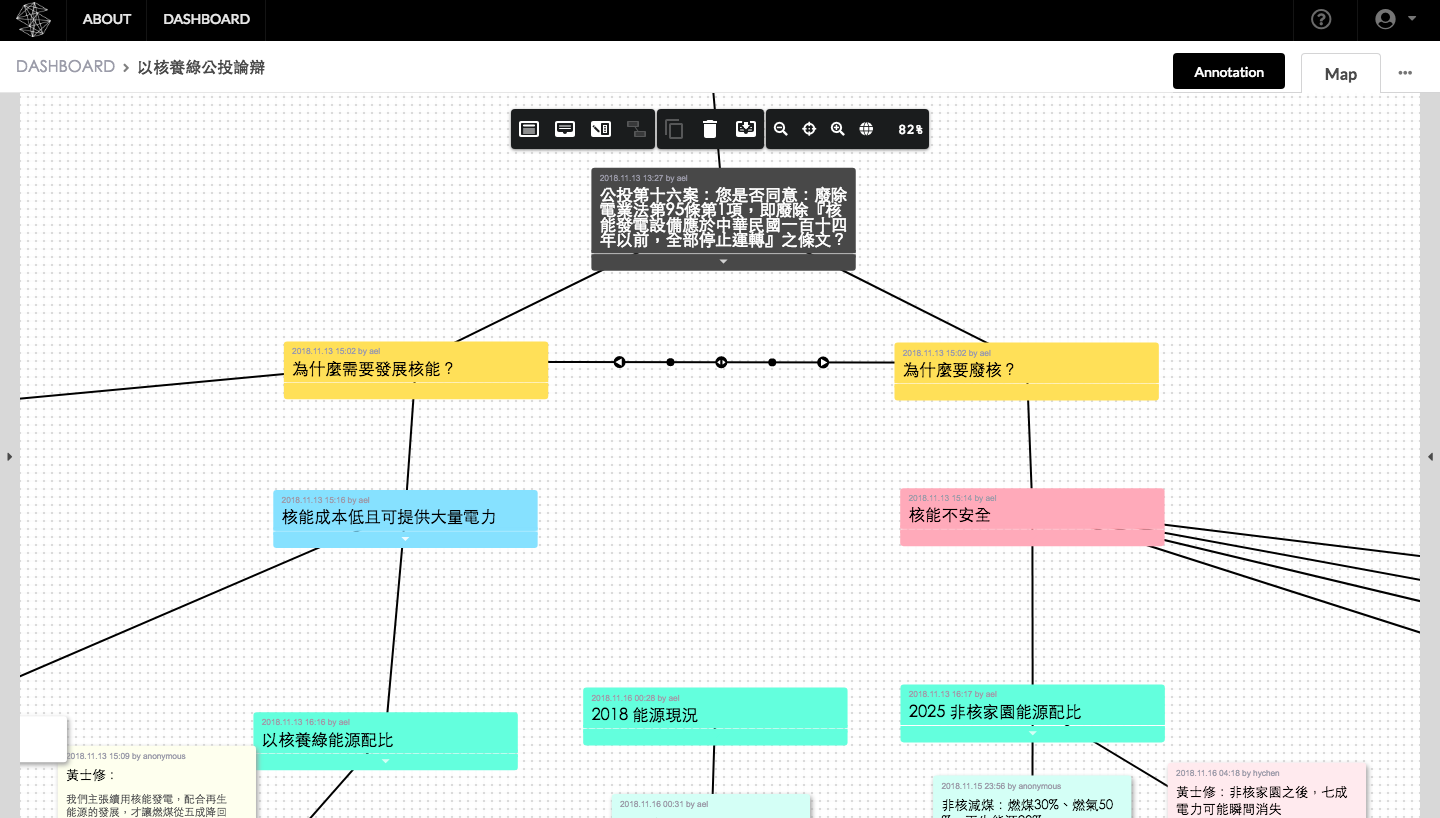
\includegraphics[width=.9\linewidth]{./images/nuclear_main_boxes.png}
\end{center}

可作為標題或是拿來群組類似之概念與論述,類似抽屜的概念可以把 Card 丟進去再做整理,如下圖為在 Box 中放入多張 Card。

\begin{center}
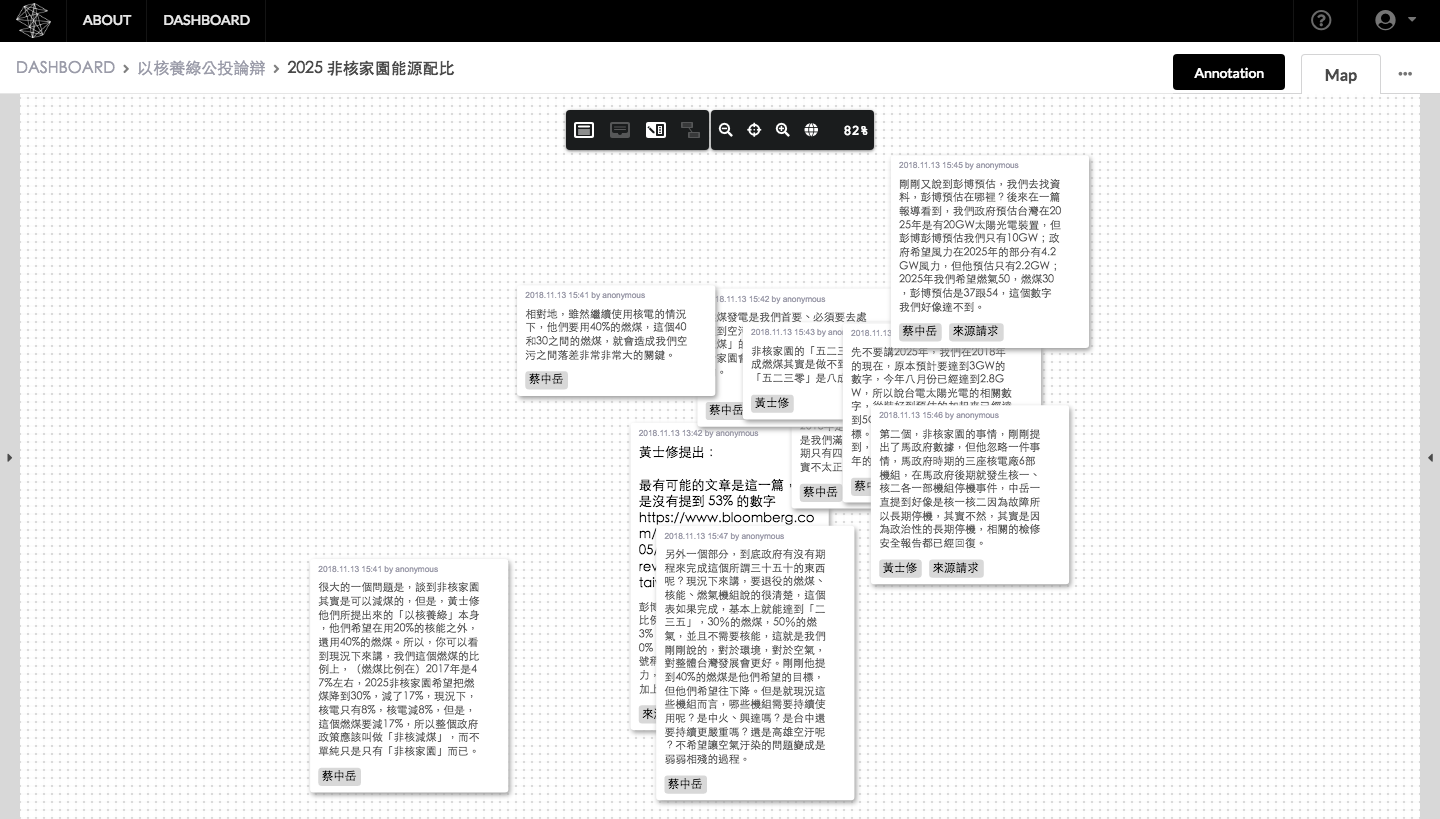
\includegraphics[width=.9\linewidth]{./images/nuclear_in_box.png}
\end{center}

最後,這些 Card 和 box 彼此之間都可連線,並標註連線關係。

\begin{center}
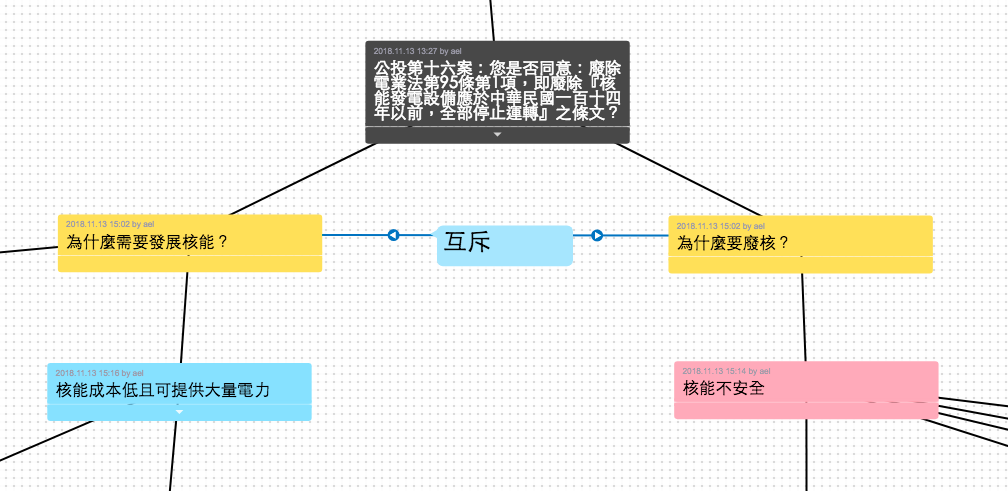
\includegraphics[width=.9\linewidth]{./images/nuclear_anti.png}
\end{center}

透過此種方式可以梳理議題脈絡、添加補充回應、補充資料來源,可看出哪些論述還未被查證缺乏資料來源、哪些問題有被完整回答,論述方所提出的解法是否還有存在其他問題等。
\begin{center}
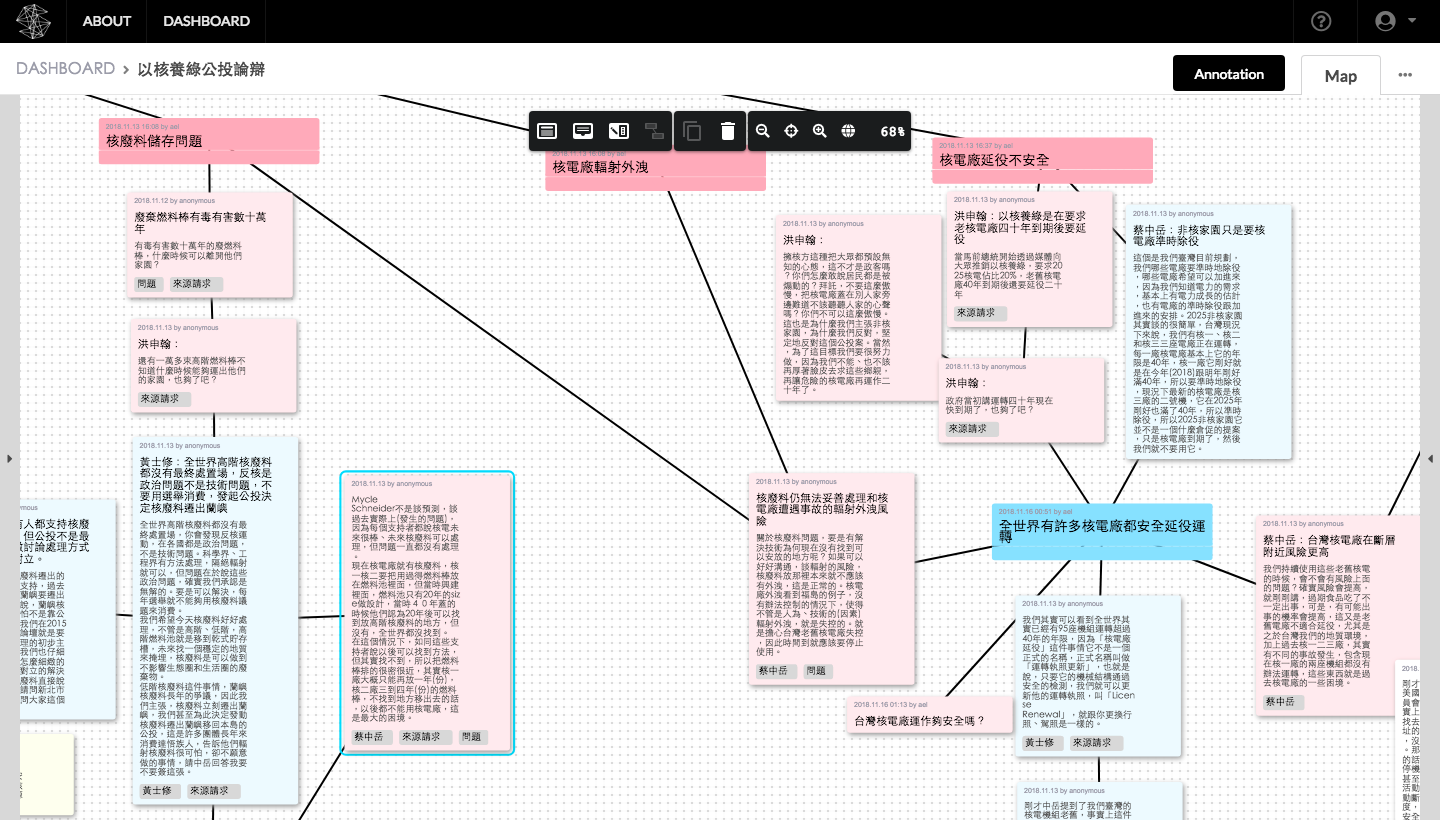
\includegraphics[width=.9\linewidth]{./images/nuclear_context.png}
\end{center}
\end{enumerate}

\item 數位化紀錄現場討論
\label{sec:org24f8f13}
以區塊鍊治理討論為例,透過投影出將討論拆解成單一概念與資料間的論證建構圖,可協助與會者在現場討論時看到已討論過的名詞定義讓知識語彙對齊,並且可檢視問答的深度與廣度,並線上補充資料連結。

\begin{figure}[htbp]
\centering
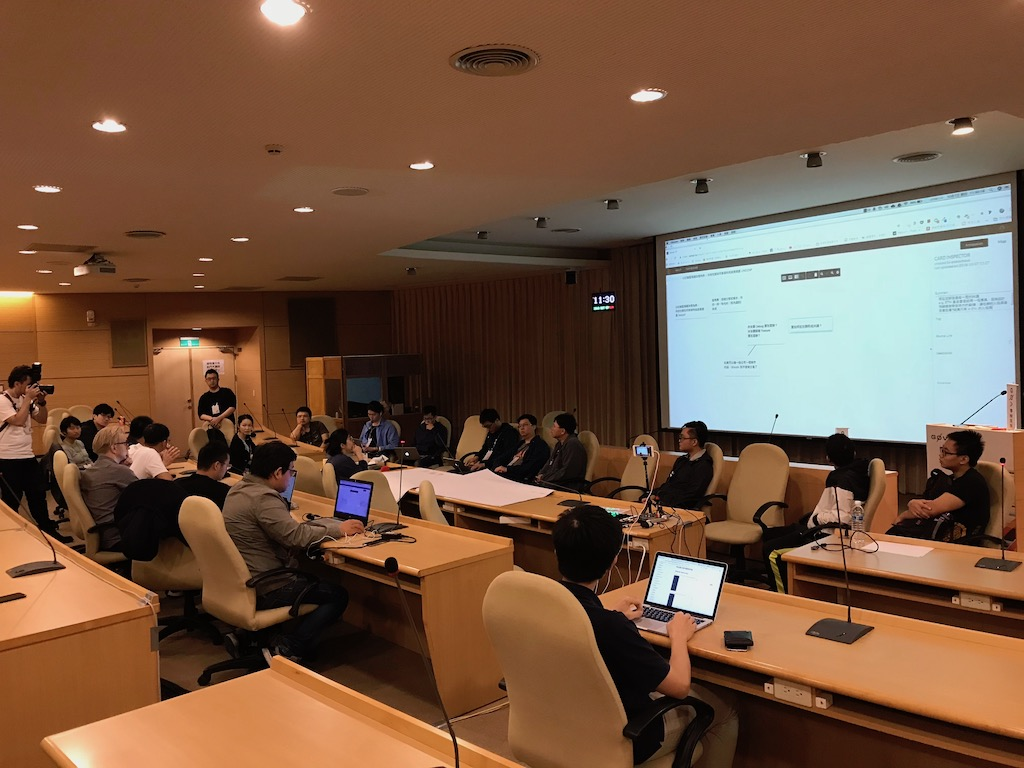
\includegraphics[width=.9\linewidth]{./images/blockchain_unconf.jpeg}
\caption{\label{fig:org54a1189}
區塊鏈治理 Unconference - G0V Summit 2018}
\end{figure}
\end{enumerate}

\item 應用成果
\label{sec:org9365708}
\begin{table}[htbp]
\caption{\label{tab:org1c5b747}
sense.tw 上 2018 年 7 月 7 日至 2018 年 12 月 16 日活躍議題地圖列表清單(本研究製表)}
\centering
\setlength{\tabcolsep}{3pt} \rowcolors[]{2}{contiYellow!5}{contiYellow!20}
\begin{tabular}{p{130pt}llllp{204pt}}
\toprule
Page Title & PV. & UPV. & Avg. & 小聚 & Page Link\\
\midrule
女性主義者給問嗎 & 3561 & 1389 & 0:55 &  & \url{https://sense.tw/map/741258c1-ad77-4701-8220-cfa887ec3a75}\\
Public Money Public Code & 1294 & 458 & 2:10 & v & \url{https://sense.tw/map/8c1c6b87-8bf8-4360-af93-5e5c917aa780}\\
g0v 黑客松關心議題整理 & 617 & 329 & 2:52 &  & \url{https://sense.tw/map/12495dd1-c79b-4292-b413-98e81be4beda}\\
民航法無人機專章引起的爭議 & 525 & 222 & 0:55 &  & \url{https://sense.tw/map/e0c2c897-cc3a-4995-8a1e-fd966572580b}\\
sense 協作模型分析 & 459 & 239 & 2:46 &  & \url{https://sense.tw/map/e1f2bd16-378f-4abc-a689-ade6937075e2}\\
台灣有網路中立性嗎? & 412 & 198 & 1:08 & v & \url{https://sense.tw/map/c03aa999-534b-4fdf-8aa5-bf45ad6f3fc1}\\
以討論區塊鏈治理為例 - 科技社群如何參與科技政策規劃 UNCONF & 384 & 317 & 8:07 & v & \url{https://sense.tw/map/8c7eec7c-4457-4c86-9ce4-fb8d1df04caa}\\
以核養綠公投論辯 & 277 & 248 & 4:59 &  & \url{https://sense.tw/map/a6a2d883-35e0-4229-a483-a6ea14c04c59}\\
UBER CASE ISSUE MAPPING - PDIS WORKSHOP IN TORONTO & 101 & 85 & 7:18 &  & \url{https://sense.tw/map/49db252f-6a55-46ea-89b2-1a88a714f54e}\\
無人機關鍵技術 & 112 & 82 & 3:00 &  & \url{https://sense.tw/map/ed9c0bfa-3399-4cef-b5ba-6f0feb69da7f}\\
議題釐清如何議題釐清 & 124 & 52 & 2:25 & v & \url{https://sense.tw/map/5890ab3c-9c1e-41a8-8c25-4a8de929a9a0}\\
如何數位治理台中? & 72 & 62 & 11:15 & v & \url{https://sense.tw/map/07802bfc-bb3d-4009-a92d-c7f29c47a1d7}\\
\bottomrule
\end{tabular}
\end{table}

截至 2018 年 11 月 30 日,共 116 人註冊。

\item 小結
\label{sec:org04ad0bc}

sense.tw 目前滿足了個人整理大量資料與數位化紀錄現場討論的使用情境,線上非同步協作則因操作門檻高,難以單純從線上吸引使用者協作。

sense.tw 工具優點:
\begin{enumerate}
\item 工具可顯現複雜議題脈絡。
\item 設計有連結的欄位可促進使用者增加連結資料,並且保留原始資料來源供讀者檢視。
\item 數位工去可在議題前期資料收集與現場討論紀錄,串接線下討論有共同知識基礎與其感興趣的主題進行討論。
\end{enumerate}
缺點:
\begin{enumerate}
\item 因功能複雜,新使用者難以上手,使用者介面易用性需提升。
\item 尚需歷史紀錄與搜尋功能協助非同步協作。
\item 難以單純由線上發起討論。
\item 對不熟悉圖像思考的人,議題地圖可讀性低,許多人不知道從何看起。
\end{enumerate}
\end{enumerate}
\subsection{線下線下議題小聚 }
\label{sec:orgf6013d3}
初期專注在開發數位工具做議題整理與爭點釐清,但發現目標之資訊實踐社群,在討論社會議題與政策尚停留在社群媒體回應留言階段,較少能夠對接到政策制定的組織論述,因此發起線下討論之議題小聚,建立資訊社群討論科技政策的參與意願與方法,目標是建立低門檻、高頻度、社群自組織的深度科技政策相關討論,讓資訊社群在下班後的時間即可抓定大原則自主發起討論,不需有專業主持人或剛性討論架構,並搭配數位工具去釐清議題和爭點,在對議題有深度討論後能以此為基礎進一步能有所行動。

議題小聚因此以資訊社群關心議題作為切入,主動尋找活躍社群合作,並搭配資訊社群舉辦之大型活動做擴散,在資訊社群熟悉的線下與網路活動空間進行討論與擴散,並且記錄操作方式公開於網路上讓網路社群採用。
\begin{enumerate}
\item 建立參與意願(議題小聚會前流程)
\label{sec:orga0676ec}
\begin{enumerate}
\item 應用場景
\label{sec:orgf100e9f}
議題小聚的應用場景建議以數位原生代為主體,配合在地社群合辦,解決場地與會眾問題。討論主題貼近與會者生活要能引起共鳴。以下以「人事時地物」五個面向來說明。

\begin{center}
\label{tab:org6d9c22b}
\rowcolors[]{2}{contiYellow!5}{contiYellow!20}
\begin{tabular}{ll}
\toprule
面向 & 說明\\
\midrule
人 & 建議對象為科技從業人員或是高中或大專學生\\
事 & 以貼近生活或環境相關主題,例如網路與物聯網\\
時 & 建議周間 19:00\textasciitilde{}22:00 或六日下午 14:00\textasciitilde{}17:00 以三個小時為單位\\
地 & 舉辦地點建議在市中心,交通便利的場所,與當地社群合辦\\
物 & 請參考下章節 - 設備需求與人員配置\\
\bottomrule
\end{tabular}
\end{center}
\item 設定討論議題
\label{sec:orgba76eb7}
科技人表面上往往對政策冷感不關心,但實際上是缺乏暸解而認為不需要知道。環境、民生、交通、經濟課題是貼近
生活的比較容易被暸解並喚起共鳴,例如教育、就業。

操作上選定都會區,找尋在地活躍技術社群,加入他們並暸解他們所關心的議題及技術,參與討論並主動分享科技政策
新知與新聞。找到核心討論目標,選定關心議題,排定時間以協辦的角色加入。
\item 尋找合作社群
\label{sec:org1a0c0f0}
想第一手接觸各縣市的科技人,透過在地活躍的技術社群會是最簡便的方式。科技圈因為技術不斷的演化及進步,需要
時時更新科技新知及知識背景與深度,往往會以一種類讀書會的形式聚集在一起,將零碎的時間組織起來透過分享學習
的方法來克服軟體技術迭代速度。透過社交軟體,如 Facebook 、Slack 、Telegram 、Blog 這類的軟體找尋合作的當地社群,口碑、與過往的聚會記錄都是可以互相暸解的方法。選定後實際參與聚會可以更加暸解活動屬性,加上與主持人深度交談交換辦活動的概念與想法。之後就是敲定舉辦小聚的時間,一般建議一場 3 個小時為主,時間以周六或平日晚上。
並保持 2 周以上的宣傳時間。

\item 網路宣傳
\label{sec:orga5f6849}
擬定宣傳稿並針對社群屬性以及習慣之溝通社群媒體擴散,例如可以發起 Facebook 活動頁作為宣傳。內文範本如下:
\textbf{【你不關心政策,政策將遠離你】}

到底要怎麼做,政府才會聽科技社群的意見?帶著你關心的議題一起來行動!在政策搞到我們之前,有沒有機會提早把聲音送進政府,讓政策制定跟得上時代。
如果把自由軟體圈習慣的開放協作流程應用到科技政策規劃,是否能讓政策能更容易迭代學習,更貼近民間真實的需求?

\textbf{【想要參與政策,如何開始實作】}

議題釐清小聚透過協同討論找出議題問題點、相關政策、法規,切入問題核心。透過組織思維把論述拉到可以跟政府對接的程度,才能提出政府會買單的提案。
這一套組織心智思維與資料的方式,同樣適合用於創業、專案規劃、設計與行銷推廣等面向。
在本活動中,將會使用到 Sense.tw 團隊所開發的 Sense Map 套件,進行議題討論與結果歸納整理,對於有興趣在團隊中導入議題協同討論工具的朋友,歡迎參加
\item 設備需求與人員配置
\label{sec:orga1ee2db}
設備需強烈建議需要網路查資料,需要可以共享畫面的投影機或電視。人員配置建議需要三以上,列表清單如下。
\begin{enumerate}
\item 設備需求
\label{sec:org861dd7c}
\begin{enumerate}
\item 20 人左右的場地
\item 投影機或電視
\item 無線網路
\item 四色便利貼,白色壁報紙
\item 簽字筆數隻
\item 名片收集箱
\item 錄音設備,拍照設備
\end{enumerate}
\item 工作人員配置
\label{sec:org39b1430}
\begin{enumerate}
\item 主持人
\item 反方角色扮演者
\item 會議紀錄者,用 hackmd 或用 sensemap 記錄
\end{enumerate}
\end{enumerate}
\end{enumerate}
\item 回應論證建構討論方法
\label{sec:org5b9a1f3}
現場討論方法採滾動式修正,主要發現為:

\begin{enumerate}
\item 要求精確名詞定義以釐清不同領域的名詞(Ground Term),光是釐清名詞定義就可協助準確定義問題。
\item 問出更深度問題(QBQ)。由對議題理解較深的老手帶新手,透過問答思辨能問出更深度的問題與如何讓更多人理解爭點。
\item 唱反調跟專家回饋可提高對議題的了解跟討論深度及品質。
\item 要求資料來源佐證資料可提高對議題的了解跟討論深度及品質。
\item 參與者組成多元性增加議題討論深度與廣度。
\item 跨時間地域的線上空間 (cyber space)與數位工具可讓現場討論被紀錄與當場補充資料,也可以延續討論,例如線上共筆、線上討論區。圖像化的數位工具如 sense.tw 可讓聚焦。
\item 線下聚會可連結對議題有興趣的參與者,引發後續討論。
\item 不追求一次有具體討論結論,而是創造頻繁而低成本的討論(Micro Activity),慢慢釐清議題與建立參與意願。
\end{enumerate}

目前已驗證前述之回應論證評估模型 \citep{guba01} ,但尚未達到網路效應(network effect)之臨界點,尚無法有代表性涵蓋一個議題特面向之利害關係人。
\begin{enumerate}
\item 活動當天操作流程
\label{sec:org813973f}
提早一個小時到現場佈置及測試活動設備,架設活動立牌、測試投影機、安排座位及入口動線、名片 e-mail 投放箱

\textbf{【活動議程】}
開場 (10 分鐘)
\begin{itemize}
\item sensen.tw 組織介紹 (5mins)
\item 活動目的介紹 (5mins)
\item 規則介紹 (20 分鐘)
\begin{itemize}
\item 四色便條紙用途介紹
\item 發言權杖使用
\item 選擇反方扮演人
\item 求資料來源
\item 時間控場
\item 與會者自我介紹
\end{itemize}
\item 活動開始 (120 分鐘)
\begin{itemize}
\item 提問
\item 問題回覆
\item 補充資料
\item 列舉利害人關係
\end{itemize}
\item 結束 (30 分鐘)
\item 各組小結
\item 介紹 vTaiwan,join, sesen.tw map
\end{itemize}

主持人開場與介紹儘量簡短,並快速的說明便利貼顏色規則。

\begin{center}
\label{tab:org723e647}
\rowcolors[]{2}{contiYellow!5}{contiYellow!20}
\begin{tabular}{lll}
\toprule
 & 資料輸入種類 & 顏色\\
\midrule
 & 問題 & 紅色\\
 & 解法與回答 & 藍色\\
 & 補充資訊 & 綠色\\
 & 利害關係人 & 黃色\\
\bottomrule
\end{tabular}
\end{center}

活動大部份的時間留給與會者自我介紹及討論。自我介紹每人 30 秒,以三個標籤用以說明描述個體,例如:

\begin{itemize}
\item 網路前端工程師
\item 自由軟體推廣者
\item 關心綠色能源
\end{itemize}

用便利貼製作名牌,放在桌前,用為交流及稱呼使用。主持人開始拋出問題,視情況請與會者發言。活動進行到中途
適時加入「利害關係人」透過反方立場觀察問題的角度的不同,來深掘問題核心建立論述強度與角度。補充資料會讓
想法變論點,論點變論述。透過大量佐証資料而非以一堆「我認為」、「我想」、「我猜」、應該」等這類不客觀,
流於情緒、謠言與假設性言論。當問題或解法被提出,要求佐証資料上網 google 即時紀錄查實,這個動作會大大影
響發言品質,因為言論經過思考記綠核實的關係而變得更好。

公民教育往往較不重視以致於大眾普偏對開會、討論、公開辨論、與發表意見等都缺乏方法與技巧。議題小聚工作坊的
流程就相當重要,人數的多寡,決定了發言規則的選定。即時紀錄是關鍵,有紀錄才能閱讀與思考,語言可以快速溝通
但記憶只有 20mins 就會被其意見擠出大腦思考列上。圖像式的記憶又比文字來的有效。Map 類將文字與文字的建立
關聯網路也比條列式的文字來的有效用。資料輸入預先以顏色作為分類,資料可快速分類過濾。

議題小聚每次約三個小時,第一次的操作往往只能達到知識語彙對齊(well-informed),而第二三次的操作透過閱讀地圖與記錄,可快速的彌補資訊落差。但之後又會因為資訊量大,而只會有少數人可以理解的人會持續關心相關議題。
\end{enumerate}
\item 會後擴散
\label{sec:org7d0a4e1}
收集與會者名片或 e-mail,用 sensemap 整理會議記錄,並主動邀請參與者參加線下討論,會後發佈當天討論的結論,並在三天內發送會議記錄,將與會者加入 mailing list 討論串內,發佈當天活動 blog 記錄。籌劃下次的活動,並延續當天討論的內容發展,進行下一次的循環。
\item 應用成果
\label{sec:org2618b7e}
截至 2018 年 12 月 20 日為止,共計舉辦 9 場議題小聚如下表。初期由本團隊發起並主動接洽北中南資訊社群,討論主題如:區塊鍊、數位治理,並且使用本計劃開發之意見整理工具 sense.tw 做數位紀錄,數位工具之紀錄使線下之討論可擴散給更多關心此議題的社群參與者,及非同步協作補充資料。在 2018 年底開始造成社群擴散效應,有資訊社群主動聯絡自行發起議題小聚,如學生計算機年會 SITCON 參與者發起「資訊教育」議題小聚;李梅樹紀念館發起在台北舉辦「文化組織如何數位開放」,並將於 2019 年持續在台北、台中舉辦延續之議題小聚討論文化組織之資訊系統標案。

\begin{table}[htbp]
\caption{\label{tab:org4aa117e}
議題小聚活動列表清單(本研究製表)}
\centering
\scriptsize \setlength{\tabcolsep}{3pt} \rowcolors[]{2}{contiYellow!5}{contiYellow!20}
\begin{tabular}{p{80pt}lllp{70pt}lp{90pt}l}
\toprule
活動名稱 & 日期 & 人數 & 地區 & 參與者背景 & 年齡 & 記錄連結 & 網路擴散\\
\midrule
COSCUP Workshop 議題小聚 & 2018/08/12 & 10 & 台北市 & 律師、工程師、業務、退休 CEO & 16-65 & \url{https://sense.tw/map/8c1c6b87-8bf8-4360-af93-5e5c917aa780} & 458\\
網路中立性議題小聚 & 2018/09/13 & 29 & 台北市 & 企業公關、公務員、出版業從業人士、學生、工程師 & 20-55 & \url{https://sense.tw/map/c03aa999-534b-4fdf-8aa5-bf45ad6f3fc1} & 198\\
區塊鏈治理 Unconf & 2018/10/17 & 40 & 台北市 & 公務員、公共行政學者、記者、區塊鏈研究員、人文科系學生、積極公民 & 20-55 & \url{https://sense.tw/map/8c7eec7c-4457-4c86-9ce4-fb8d1df04caa} & 317\\
數位治理台中議題小聚 & 2018/10/20 & 15 & 台中市 & 台中維基、自由軟體愛好者社群	議題小聚 & 20-55 & \url{https://sense.tw/map/07802bfc-bb3d-4009-a92d-c7f29c47a1d7} & 62\\
台南議題小聚 & 2018/10/30 & 7 & 台南市 & 南科工程師、成大學生 & 25-55 & N/A & \\
MOPCON 議題小聚 & 2018/11/04 & 25 & 高雄市 & 濁水溪以南 25 個資訊科技社群 & 25-55 & N/A & \\
文化組織如何數位開放? & 2018/12/02 & 20 & 台北市 & 博物館從業人員、資訊工程師、學生、科技藝術家、傳統藝術家、維基百科社群等 & 15-55 & \url{https://g0v.hackmd.io/129ZYA-GQFKcS0gtVIYvFA} & 1542 (直播)\\
先不管課綱,你想要怎樣的資訊素養? & 2018/12/20 & 20 & 台北市 & 大學生、高中生、工程師 & 15-35 & \url{https://sense.tw/map/1c2220b6-75b1-40dc-816d-13d57d0ddfb3} & 42(擴散人次待補)\\
\bottomrule
\end{tabular}
\end{table}
\end{enumerate}

\subsection{線上線下串接案例 }
\label{sec:orgd4f33da}
前述分別介紹線上意見整理工具 sense.tw 與線下的議題小聚,此節以案例介紹如何串接線上數位工具與線下線下討論,加深網路社群討論科技政策之品質。
\begin{enumerate}
\item Public Money, Public Code
\label{sec:orgdc15fce}
Public Money, Public Code 為國際開源社群長期推動由政府資助開發的軟體應開放原始碼的運動\footnote{Public Money, Public Code 活動由歐洲自由軟體基金會發起,要求制定法律,明訂以公務機關的經費,為公務機關開發的軟體,必須以自由開源軟體授權釋出,截至 2018/12/21 為止全球已有 158 個組織與 19130 個人已經連署公開信表達支持。詳見 \url{https://publiccode.eu/zh-tw/}。}。在開源人年會(COSCUP)中大高雄 Linux 協會(KaLUG)與樹黨\textsuperscript{\ref{org2853c6b}}開始討論,於是舉辦之議題工作坊以此為主題進行討論。

流程如下\footnote{以下 Public Money Public Code 討論流程改寫自本計劃 2018 年 8 月 17 日部落格〈COSCUP 小記:科技社群如何參與科技政策規劃(我們需要更多 Pizza!)〉,連結:\url{https://medium.com/sense-tw/community-tech-policy-coscup2018-1cefe60b38c3}}:
\begin{enumerate}
\item 先使用 sense.tw 在網路上整理相關問題與討論架構,分類問題與找到的相關資料作為回答
\begin{center}
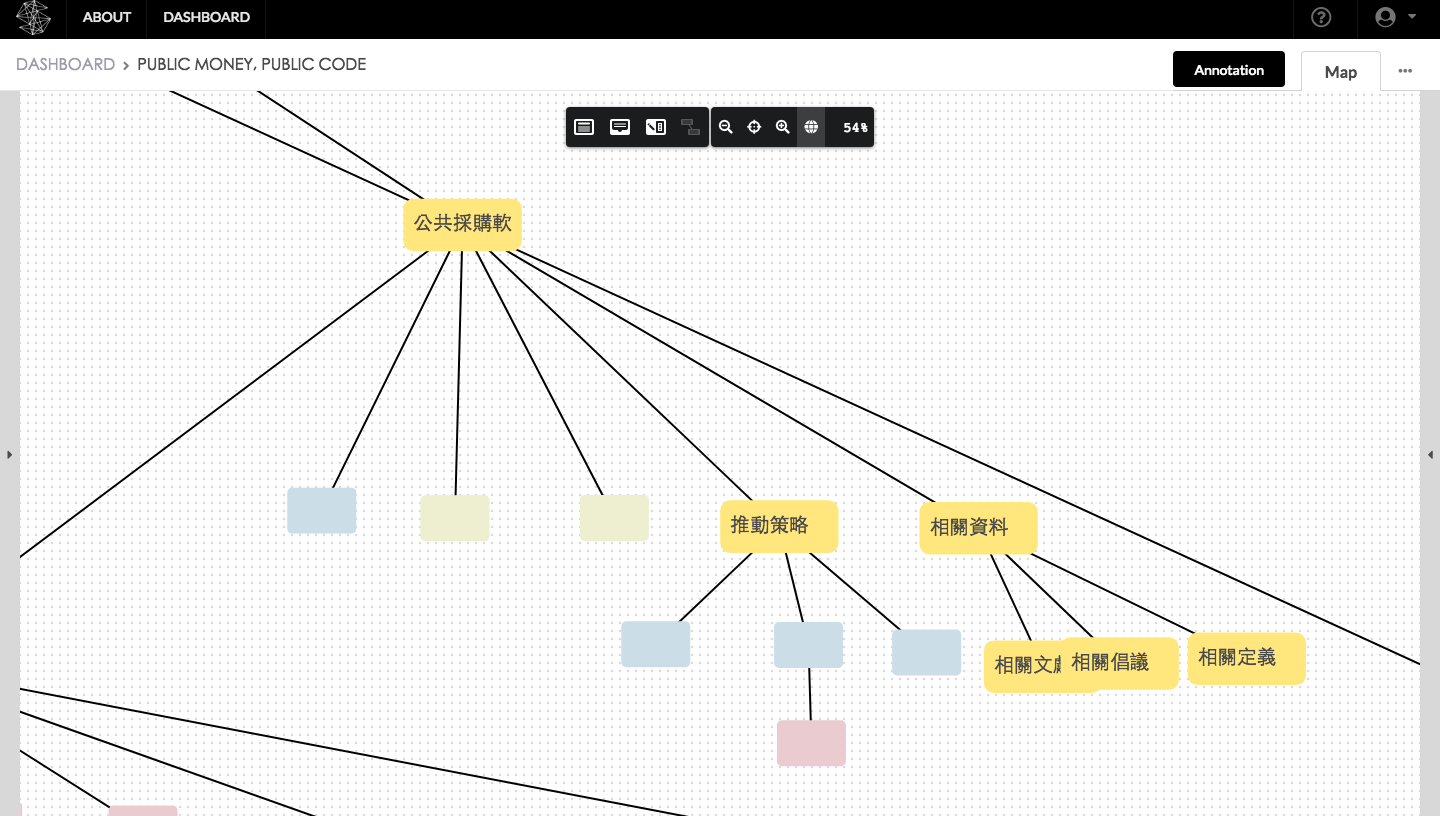
\includegraphics[width=.9\linewidth]{./images/pmpc2.png}
\end{center}
\item 在資訊社群大量出沒的開源人年會舉辦線下議題小聚工作坊,以問答、名詞定義、利害關係人、補充資料來源之方式釐清議題。
這一場有三位長期參與開源專案的工程師(Shawn、宗翰、Tim)、一位資通訊產業協會的前輩(Vincent)、一位前公務員(Weilun)。我們將便利貼分為四種顏色:
\begin{itemize}
\item 問題(紅色)
\item 解法/回答(藍色)
\item 補充資訊(綠色)
\item 利害關係人(黃色)

\item 步驟:
\end{itemize}
\begin{enumerate}
\item 請大家對這個主題提出相關的問題(紅色)
\item 結果就必須去作名詞定義、釐清、回答(藍色)
\item 在名詞定義過程中需要補充資訊(綠色):補充國內法規、國外作法、政府補助方式。加上問題和解法會牽涉到的利害關係人(黃色)
\item 讓參與的人意識到提出他的解法會是別人的問題,因此引導預想可能會被質疑的面相。
\item 討論過程中覺得是誰的發言很重要,所以也把發言人的名字標上去。
\begin{center}
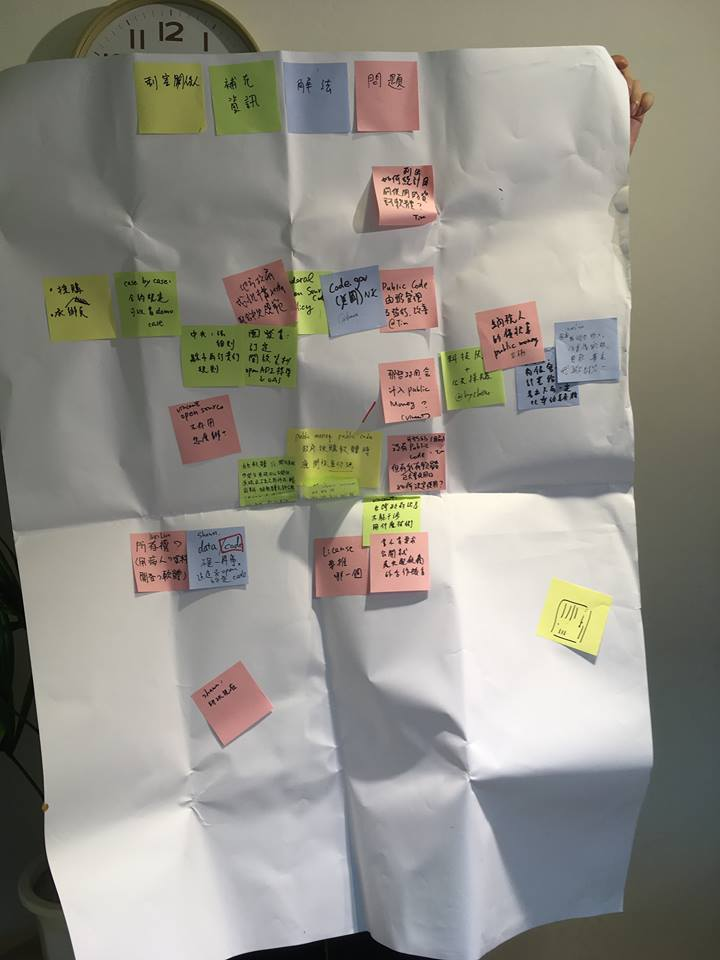
\includegraphics[width=.9\linewidth]{./images/pmpc.png}
\end{center}
\begin{enumerate}
\item 討論內容:
\end{enumerate}
\item (名詞定義)開源軟體與自由軟體差別:不是公布原始碼就有達到 Public Code 的標準
\item (問題)Public Money Public Code 指的是政府採購既有軟體產品還是政府出資開發的程式?
\item (回答)確認 PMPC 的意思,今天宗翰、Tim、Shawn 認為是政府花出去的請業者開發的錢,所寫的新開發的軟體/程式碼需要開源。而不是指政府都需要採購開源軟體。
\item (問題)什麼是 Public Code?
\item (回答)public code 對於非工程師,會想到資料安全性和隱私權的問題。這邊有釐清 public code 不等於 open data,code 跟 data 是分開的。
\item (問題)那 Public Code 要由誰管理和維護和訂定標準?
\item (補充資訊)美國有 code.gov
\item (補充資訊)台灣目前是 open data 標準由國發會制定,但是地方政府可以參考但不定要遵循
\item (問題)什麼是 Public Money?
\item (回答)需要釐清 Public money 是什麼意思,哪些經費來源所開發的程式碼需要開源。本來工程師覺得定義很簡單,就是納稅人的錢,但維倫和 Vincent 有提到政府收入有很多種來源,並非全部都來自稅收,而且政府有許多補助研究案,會採取政府 49\%,企業 51 \% 的方式出資,因為鼓勵創新,研究成果歸企業主。
因為時間不夠,很多關鍵問題釐清了但很可惜沒又繼續討論下去,於是我們有將這個討論結果整理到線上的工具,希望能夠延續討論。這可以回答工作坊有些參與者質疑為什麼需要開發線上工具做議題釐清,因為線上可以:
\begin{itemize}
\item 非同步協作重複這個線下的討論 cycle,使討論可以延續
\item 線上工具比線下更容易加補充資料
\end{itemize}
\end{enumerate}
\item 將現場討論紀錄在 sense.tw 並在網路上延續討論,例如互相標註來源請求、補資料、修正說法。
在線下討論會後,持續在線上做議題釐清,這邊以 hychen 和 kevin 在 sense.tw 吵 Public Money Public Code 為例。
\begin{center}
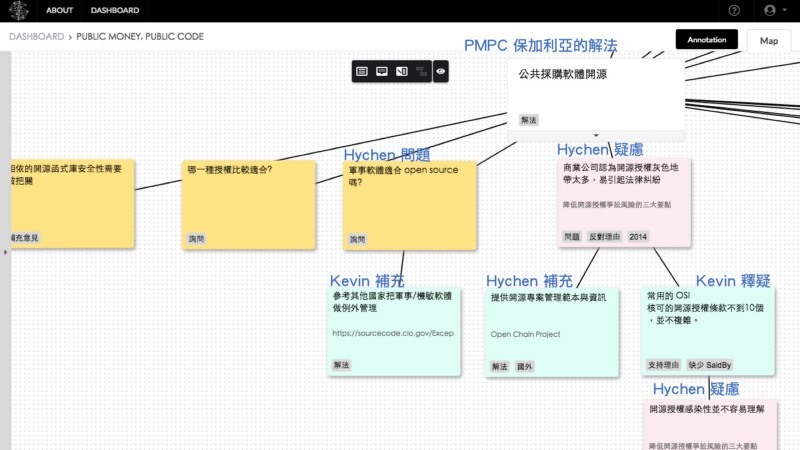
\includegraphics[width=.9\linewidth]{./images/pmpc-hychen-kevin1.jpg}
\end{center}
上面的截圖中,Hychen 先盤點了 Public Money Public Code 的一些大點,在公共採購軟體開源這個保加利亞的政策下,hychen 列了幾個問題,包括 — — 軍事軟體適合 open source 嗎?商業公司認為開源授權灰色地帶太多,易引起法律糾紛。並且都附上資料來源。kevin 就針對這兩個問題補充了資訊,也附上連結,hychen 則進一步針對 kevin 的回答提出問題。
在下圖中,他們也用 tag 互相標注對方的卡片「來源請求」、「缺少 SaidBy」,要求對方的論證品質,或進一步根據對方提供的資料修改自己的論述。hychen原本的紅色卡片是說開源軟體容易被駭,但 Kevin 覺得是假議題,是在開源圈裡早就被廣泛澄清的資訊;於是 hychen 修正為,開源容易被有心人針對撰寫攻擊程式。
\begin{center}
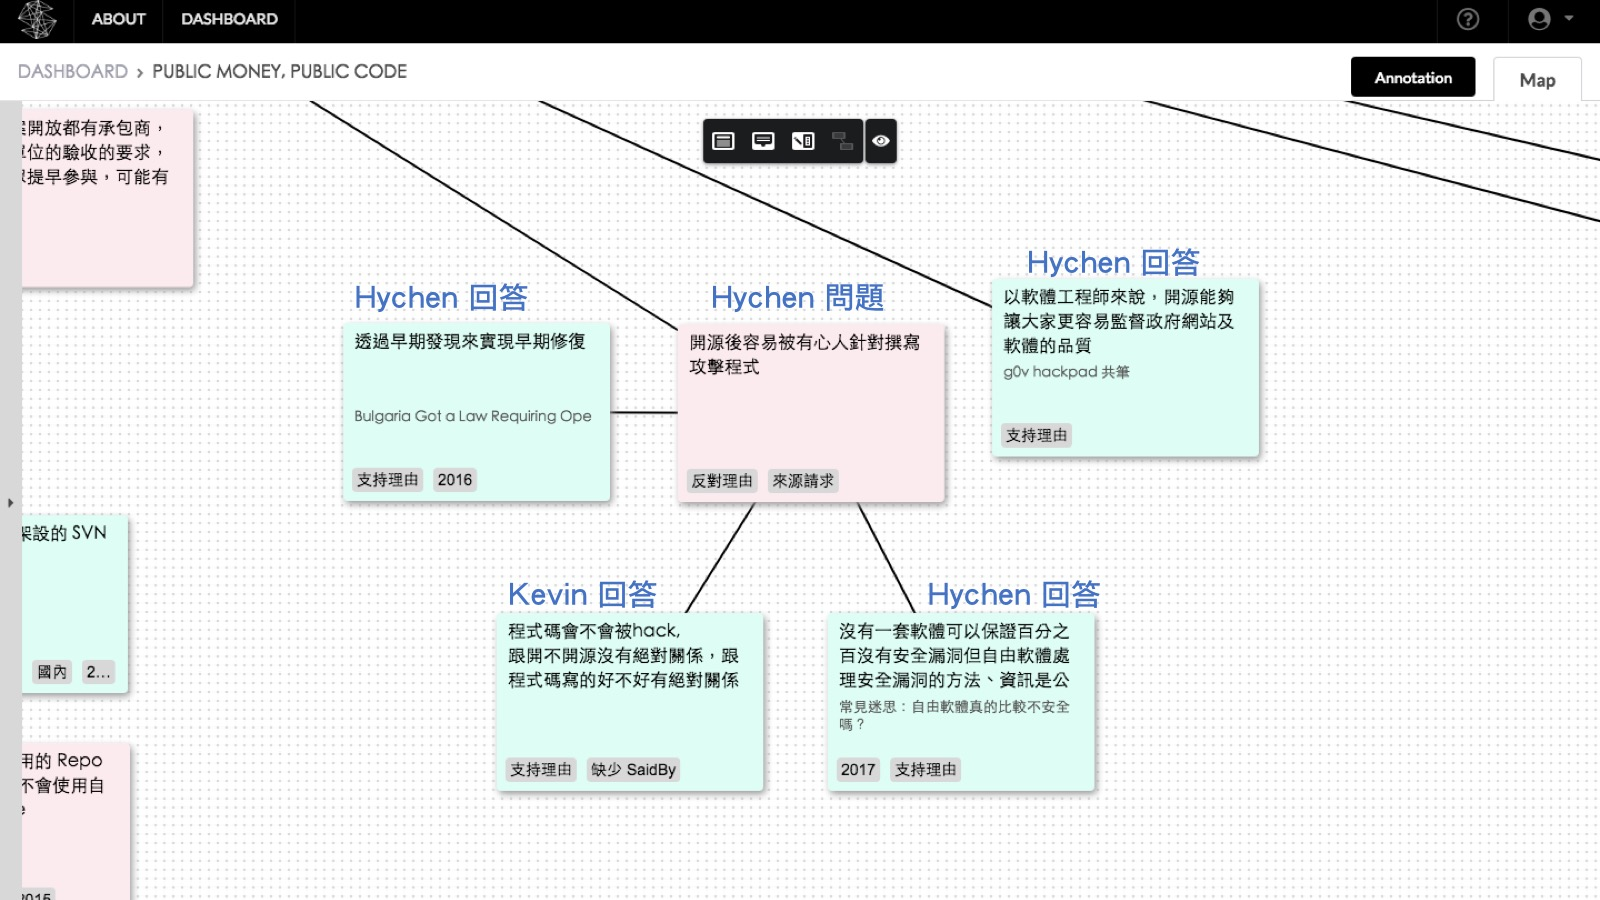
\includegraphics[width=.9\linewidth]{./images/pmpc-hychen-kevin2.jpg}
\end{center}
\item 會後有人整理成說帖文件去與地方政府溝通
\end{enumerate}
\begin{enumerate}
\item 小結
\label{sec:orgaf0ff43}
這是第一場議題小聚,後來的議題小聚延續這樣問題(questions/concerns/problems)、解法(answers/solutions)、利害關係人(stakeholders)、名詞定義(definition)、立場(statements/claims)的討論。利害關係人對於非公共行政、專案管理背景的人來說是個新的思考事情的維度,但熟悉網路治理多邊利害關係人模式的社群參與者馬上可以抓到這個概念。名詞定義則是在網路上特別需要去聚焦的部分,以及跨專業時需要去確認的東西,才能建立共同語彙,推進實質討論。想要用這樣回應的方式讓社群可以在同溫層裡面意見徵詢,透過同溫層滾同溫層的模式,去做到論點交換,對話迴圈要雪球滾起來,找到同溫層內的共識。在數位工具上則是能做到,當彼此可以看到彼此的資料來源的時候,才能知道為何得出那樣的論證。
\end{enumerate}
\item 網路中立性
\label{sec:org3eed1fd}
\begin{enumerate}
\item 設定議題
\end{enumerate}
網路中立性為第二場議題小聚,議題設定選擇為網路社群一直關心的「網路中立性」和「境外封網」\footnote{台灣近年境外封網事件整理:\url{https://bit.ly/2PWFkZ7}。}作為議題,網路社群基本上支持網路中立性與反對境外封網,雖然後來經過現場討論議題釐清之後,發現其實是兩個不同的議題。
\begin{enumerate}
\item 初步整理網路資料並創建活動頁面做網路擴散:
\begin{itemize}
\item 創建活動頁面:\url{https://www.facebook.com/events/453192175172987/} ,依靠臉書做擴散,既可以收集對此議題感興趣者的名單,又可提供線上空間讓參與者可丟連結和參與共筆紀錄。
\item 事先整理整理台灣封網事件的時間軸:\url{https://bit.ly/2PWFkZ7}。
\end{itemize}
\item 議題小聚現場討論
\begin{enumerate}
\item 創立線上共筆與線上論證圖 sense.tw 紀錄
\end{enumerate}
\begin{enumerate}
\item 指定一人做紀錄。
\item 將 sense.tw 論證圖投影至投影幕幫助理解論點討論進度與爭點。
\end{enumerate}
議題地圖連結: \url{https://sense.tw/map/c03aa999-534b-4fdf-8aa5-bf45ad6f3fc1}
\begin{enumerate}
\item 討論方式介紹:介紹問答、名詞定義、要求補充資料來源、利害關係人的討論方法。
\item 自我介紹:讓參與者彼此認識,並且認知到每個參與者都有其關心的面向與可貢獻的討論方向。此次參與者組成非常多元,有學生、工程師、公關、公務員、議題倡議者。
\item 討論方法:
\end{enumerate}
\begin{enumerate}
\item 同步以線下海報、便利貼和 sense.tw 做討論。
\item 同時間只有一人發言,但任何人都可以現場筆電補充資訊或遠端線上補充資訊,並且在討論過程中所舉出的事例都需要說明資料來源,實際在討論過程中也有不講話的工程師默默補了很多連結,NCC 僱員提供已公開的研究資料、議題倡議者提供國外 NGO 的倡議文件等。
\item 未有指定主持人,只有指定唱反調者挑戰既有討論、要求名詞定義與資訊來源。
\begin{enumerate}
\item 討論內容:
\end{enumerate}
\end{enumerate}
\begin{center}
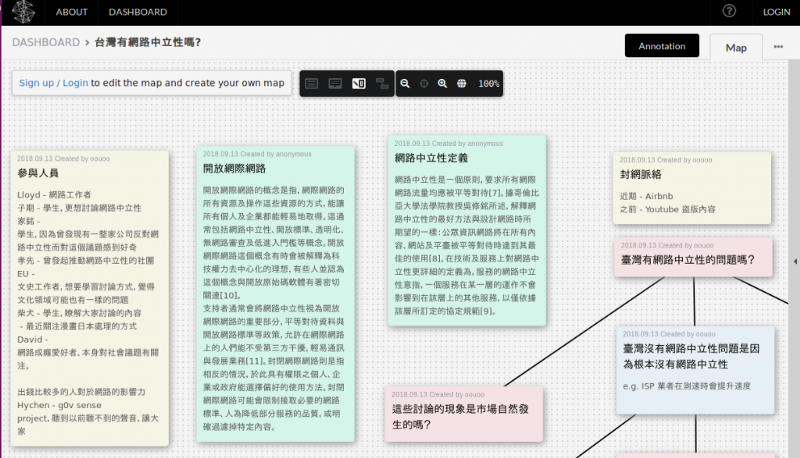
\includegraphics[width=.9\linewidth]{./images/net-neutrality1.png}
\end{center}
\begin{enumerate}
\item 問題:首先問什麼是網路中立性,就發現跟境外封網的定義不同,決定討論網路中立性。
\item 名詞定義:使用維基百科對於網路中立性的定義。
\end{enumerate}
「網路中立性是一個原則,要求所有網際網路流量均應被平等對待。據哥倫比亞大學法學院教授吳修銘所述,解釋網路中立性的最好方法與設計網路時所期望的一樣:公眾資訊網路將在所有內容、網站及平臺被平等對待時達到其最佳的使用。在技術及服務上對網路中立性更詳細的定義為,服務的網路中立性意指,一個服務在某一層的運作不會影響到在該層上的其他服務,以僅依據該層所訂定的協定規範。\footnote{「網路中立性」維基百科定義,2018 年 9 月 13 日摘自 \url{https://zh.wikipedia.org/wiki/\%E7\%BD\%91\%E7\%BB\%9C\%E4\%B8\%AD\%E7\%AB\%8B\%E6\%80\%A7}}」
\begin{enumerate}
\item 問題:台灣真的有網路中立性的問題嗎?
\item 回答:台灣目前沒有網路中立性,因為網速會因為內容而不同(個人實測)。
\item 問題:為什麼?
\item 回答:因為 ISP 對接上有收費。
\item 問題:什麼是 ISP (Internet Service Provider)?
\item 定義:狹義為網路提供商,廣義進一步包括網站提供者, Google 作為網站服務提供者,有自己的海纜。
\item 問題:所以是怎麼對接收費的?
\item 回答:台灣有四個網際網路交換中心,有上架費,但使用率都不高。
\item 問題:什麼叫做使用率不高,誰會跟網際網路交換中心對接?
\item 回答、利害關係人:畫了個網路基礎建設服務商線路串接的關係圖,如下圖。(提供這些資訊的參與者當初只是為了想要省網路費而查清楚,並且現場搜尋資料)
\end{enumerate}
\begin{center}
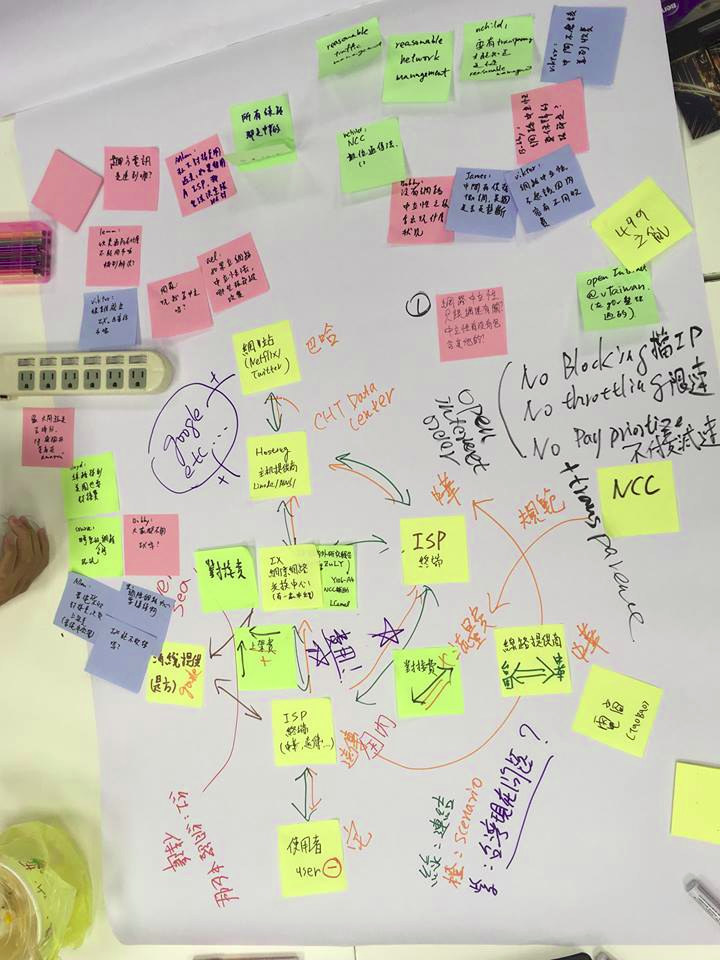
\includegraphics[width=.9\linewidth]{./images/net-neutrality-ISP.png}
\end{center}
\begin{enumerate}
\item (延續討論)
\end{enumerate}
最後總算讓大家搞懂,因為 ISP 業者間的上架費與不同廠商硬體纜線成本,使用者取得不同網站內容的網路線路成本是不同的,所以接下來要討論的價值判斷,是要讓市場機制和成本決定使用者所需要的付費或網速,還是政府為了取得資訊的公平性而要介入?有什麼可能的解法?並且丟出網路中立性三個重要原則:「No Blocking. No Throtting. No Paid Prioritization.」。
\begin{center}
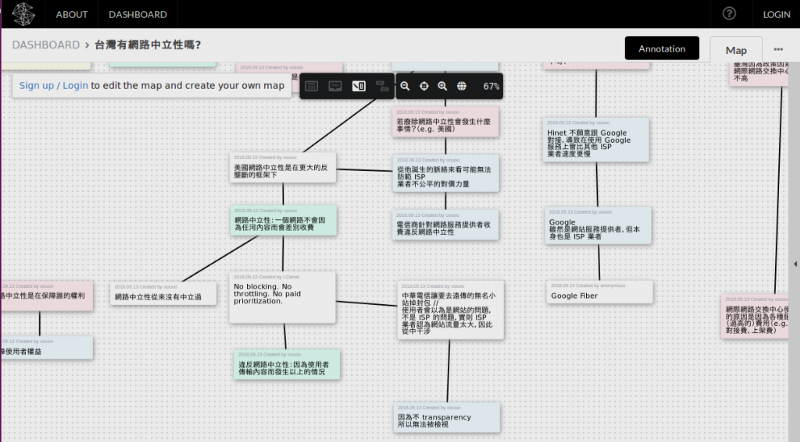
\includegraphics[width=.9\linewidth]{./images/net-neutrality2.png}
\end{center}
\item 在會後在線上持續補充資訊、參與者互相交換連絡方式
\item 整理成文章網路擴散
\end{enumerate}
\end{enumerate}
\section{結論與建議 }
\label{sec:orge2be46f}
\subsection{研究發現}
\label{sec:orgd46af54}
\begin{enumerate}
\item 溝通落差
\label{sec:orgdaaacab}
從使用者訪談中得知網路社群與政府間的溝通落差來自於視角不同與掌握資訊不同,政府應提供單一入口、易於查詢的全面政策規劃資料,而民間需將自己的知識語彙與政府對齊,並且整理出論述以便與政策討論接軌。

\item 網路社群公民參與機制分析
\label{sec:orgc2c573e}
以服務藍圖、顧客旅程圖等服務設計方法,拆解網路社群公民參與之階段為五個階段:「前期議題設定」、「議題發酵」、「正式行動」、「政府正式會議」、「政策修正」,並且針對網路社群在每個階段的接觸點做深入探討,發現在每個階段讓行動者、與會者的知識語彙對齊以梳理議題脈絡非常重要。在進入「正式行動」對政府提出訴求之前,在前期議題設定和議題發酵讓更多人關心與參與的階段,知識語彙對齊更顯重要。網路社群需先有參與意願,有參與意願後有時會因缺乏凝聚共識與議題釐清之方法,無法提出有效之論述影響政策。

\item 發展出線上線下議題釐清工具與機制
\label{sec:orgdfdbfc8}
從文獻檢閱檢視如何促進線上公民參與之討論品質,發現需增加線上參與誘因與引導公眾做議題釐清,而高頻度低成本之討論、問出深度問題、根基原始文獻之討論,可有效提升討論品質。根據文獻與訪談結果分析,發展出線上線下串接之議題釐清工具與機制。基本架構為採用群眾協作貢獻多元知識與視角,問答方式引導討論者問出更深度的問題和換位思考,並且要求名詞定義和論述需引用資料來源以做查證和知識語彙對齊,並且納入利害關係人分析視角檢視議題之不同意見。

其中本研究所開發之數位工具 sense.tw ,具備在原始文獻上註記之功能,並且能夠將論述與原始資料以論證圖等視覺化方式協助使用者整理議題脈絡、導引協助論證式思考,可用於大量資料整理與記錄實體討論使之能網路擴散。實體討論之議題小聚,則以實體討論建立網路社群之參與意願與建立對該議題關注之積極公民間之個人連結,透過參與者多元背景交換知識做知識語彙對齊,透過問答討論做議題釐清,使網路社群參與者可在業餘時間自組織鬆散討論,以低成本、高頻之方式滾動討論,逐漸深入議題核心爭點,並i搭配數位工具紀錄與在網路上延續討論和分享資料。讓每個社群可發起自己對於政策的預評估。

最好的效果是由熟悉該社群文化之社群參與者發起並延續討論,進行線下實體討論並且有線上數位記錄與資訊分享做擴散,是為網路社群自發之線上線下網路參與機制。
\end{enumerate}

\subsection{政策建議}
\label{sec:org099aa21}
本研究專注在促進民間網路社群自組織議題釐清,主動權不在政府部門手上,然而政府能夠做好資料開放作為促進網路公共政策討論之品質之基石。

\begin{enumerate}
\item 開放易搜尋與互相連結之資料補足民間與政府知識落差
\label{sec:org7edb381}
從對線上參與機制與公民參與的使用者訪談中得知網路社群因視角不同與政府產生溝通落差(見 \ref{fig:gap1} ),網路社群容易對議題、新聞做出反應,較難得知跨部會的全盤政策與各部會職掌。若政府政策相關文件只有以 PDF 檔分別放在各部會網站上,對於不熟悉各部會執掌和計畫的民間收集相關議題資料較為不便,建議除了 PDF 檔案外有網頁形式或至少有標註關鍵字和提供相關連結,方便有興趣之公民使用搜尋引擎查找。例如科技會報之「AI 行動計畫」有完整網頁介紹全面性政策\footnote{2018 年 12 月 22 日,截至行政院網站 \url{https://www.ey.gov.tw/Page/5A8A0CB5B41DA11E/a8ec407c-6154-4c14-8f1e-d494ec2dbf23} 。},只可惜缺乏連結回相關原始文件報告,只有連結新聞報導。亦可參考馬德里市政府開發之 CONSUL 的線上參與平台\footnote{該平台在線上投票、線上論壇外,亦有線上註記之功能,可參考 \url{http://consulproject.org/en/\#features}。}與美國聯邦政府 18F \footnote{18F 為美國聯邦總務署(General Service Administration)轄下之數位創新單位,此註記政策回饋功能在 2018 年 5 月拜訪開發團隊時為原型開發階段,程式碼在 \url{https://github.com/18F/omb-eregs}。}皆有開發可供民眾直接在線上註記政策網頁檔以回應政策意見之工具
,本計劃開發之 sense.tw 意見整理工具也可達到同樣功能。
\end{enumerate}
\section{附錄}
\label{sec:orgcdeedd3}
\subsection{訪談對象與訪談形式}
\label{sec:org62782c2}
\begin{table}[htbp]
\caption{\label{tab:org4c4066a}
訪談對象及訪談形式}
\centering
\rowcolors[]{2}{contiYellow!5}{contiYellow!20}
\begin{tabular}{lrlll}
\toprule
日期 & 編號 & 形式 & 身份 & 性質\\
\midrule
2018/01/10 & 1 & 半結構式 & 社群參與者 & 使用者需求訪談\\
2018/01/11 & 2 & 非正式 & 社群參與者 & 使用者需求訪談\\
2018/01/11 & 3 & 半結構式 & 社群參與者, 外部專家 & 使用者需求訪談\\
2018/01/12 & 4 & 半結構式 & 社群參與者, 外部專家 & 使用者需求訪談\\
2018/1/13 & 5 & 團體討論 & 政務官, 社群參與者 & 諮詢\\
2018/1/13 & 6 & 團體討論 & 積極公民, 社群參與者, 外部專家 & 諮詢\\
2018/1/13 & 7 & 團體討論 & 政務官幕僚, 社群參與者 & 諮詢\\
2018/1/13 & 8 & 團體討論 & NGO 工作者, 社群參與者 & 諮詢\\
2018/1/13 & 9 & 團體討論 & 社群參與者, 法人承辦 & 諮詢\\
2018/1/13 & 10 & 團體討論 & 學者 & 諮詢\\
2018/01/19 & 6 & 半結構式 & 積極公民, 社群參與者, 外部專家 & 使用者需求訪談\\
2018/01/25 & 11 & 半結構式 & 一般公民 & 使用者需求訪談\\
2018/01/25 & 12 & 半結構式 & 社群參與者, 外部專家 & 使用者需求訪談\\
2018/01/29 & 13 & 半結構式 & 社群參與者, 外部專家 & 使用者需求訪談\\
2018/01/29 & 14 & 半結構式 & 社群參與者 & 使用者需求訪談\\
2018/1/31 & 15 & 非正式 & 社群參與者 & 諮詢\\
2018/02/10 & 16 & 半結構式 & 積極公民, 媒體工作者 & 使用者需求訪談\\
2018/02/11 & 17 & 半結構式 & 積極公民, 媒體工作者 & 使用者測試\\
2018/03/01 & 18 & 半結構式 & 分析師 & 使用者需求訪談\\
2018/03/05 & 8 & 半結構式 & NGO 工作者 & 諮詢\\
2018/03/05 & 19 & 半結構式 & 法人承辦 & 諮詢\\
2018/03/05 & 20 & 半結構式 & 政務官幕僚, 設計師 & 諮詢\\
2018/03/09 & 21 & 半結構式 & 政府顧問 & 使用者需求訪談\\
2018/03/09 & 22 & 半結構式 & 事務官 & 使用者需求訪談\\
2018/03/17 & 23 & 非正式 & 前政務官 & 使用者需求訪談\\
2018/03/17 & 24 & 非正式 & 社群參與者, 外部專家 & 使用者需求訪談\\
2018/03/17 & 14 & 非正式 & 社群參與者 & 使用者需求訪談\\
2018/03/17 & 2 & 非正式 & 社群參與者 & 使用者需求訪談\\
2018/03/17 & 13 & 非正式 & 社群參與者, 外部專家 & 諮詢\\
2018/03/17 & 25 & 非正式 & 社群參與者 & \\
2018/03/28 & 26 & 半結構式 & 分析師 & 使用者需求訪談\\
2018/03/28 & 10 & 非正式 & 學者 & 使用者需求訪談\\
2018/03/29 & 20 & 團體討論 & 政務官幕僚 & 諮詢\\
2018/03/29 & 27 & 團體討論 & 政務官幕僚 & 諮詢\\
2018/03/29 & 10 & 團體討論 & 政務官幕僚 & 諮詢\\
2018/03/29 & 28 & 團體討論 & 政務官幕僚 & 諮詢\\
2018/04/02 & 7 & 半結構式 & 政務官幕僚 & 使用者需求訪談\\
2018/04/08 & 29 & 非正式 & 公務員 & 使用者需求訪談\\
2018/04/11 & 20 & 團體討論 & 政務官幕僚 & 諮詢\\
2018/04/11 & 27 & 團體討論 & 政務官幕僚 & 諮詢\\
2018/04/13 & 30 & 非正式 & 政府顧問 & 使用者需求訪談\\
2018/04/16 & 31 & 半結構式 & 分析師 & 使用者需求訪談\\
2018/04/20 & 32 & 半結構式 & 分析師 & 使用者需求訪談\\
2018/04/25 & 20 & 團體討論 & 政務官幕僚 & 諮詢\\
2018/04/25 & 27 & 團體討論 & 政務官幕僚 & 諮詢\\
2018/05/04 & 20 & 團體討論 & 政務官幕僚 & 使用者需求訪談\\
2018/05/21 & 26 & 半結構式 & 分析師 & 使用者測試\\
2018/07/07 & 33 & 非正式 & 公務員 & 使用者測試\\
2018/07/07 & 34 & 非正式 & NGO 工作者 & 諮詢\\
2018/07/07 & 35 & 非正式 & 社群參與者 & 諮詢\\
2018/07/07 & 36 & 非正式 & 社群參與者 & 使用者測試\\
2018/07/07 & 37 & 半結構式 & 社群參與者 & 使用者測試\\
2018/07/13 & 38 & 非正式 & 設計師 & 諮詢\\
2018/08/02 & 39 & 半結構式 & 法人承辦 & 使用者需求訪談\\
2018/08/02 & 34 & 半結構式 & NGO 工作者 & 使用者需求訪談\\
2018/08/04 & 40 & 半結構式 & 社群參與者 & 使用者測試\\
2018/08/04 & 41 & 半結構式 & 社群參與者 & 使用者測試\\
2018/08/20 & 9 & 團體討論 & 社群參與者 & 諮詢\\
2018/08/20 & 20 & 團體討論 & 社群參與者 & 諮詢\\
2018/08/20 & 2 & 團體討論 & 社群參與者 & 諮詢\\
2018/08/20 & 27 & 團體討論 & 社群參與者 & 諮詢\\
2018/08/20 & 42 & 團體討論 & 社群參與者 & 諮詢\\
2018/08/20 & 8 & 團體討論 & 社群參與者 & 諮詢\\
2018/10/30 & 43 & 非正式 & 學者 & 諮詢\\
2018/12/3 & 37 & 半結構式 & 社群參與者 & 使用者測試\\
\bottomrule
\end{tabular}
\end{table}
\subsection{數位原民參與訪談大綱}
\label{sec:org60fdf7e}
\begin{enumerate}
\item 訪談目的
\label{sec:orge745585}
訪談參與政府政策制定的網路社群外部專家的相關經驗,從案例分享,歸納出建議政府與積極公民的協作準則、可參考的流程、範本,或修正寫作與訪談方向。
\item 訪談對象
\label{sec:org53fcd91}
訪談十位積極參與(科技)政策制定的社群朋友(以下任一條件):
\begin{itemize}
\item 積極公民,會分享轉貼、評論公共事務。
\item 整理過議題資訊的懶人包或是論點、事實整理。
\item 發起過網路 campaign。
\item 在網路組織線下實體活動。
\item 參與過政策遊說。
\item 參與過政府專家會議。
\item 參與過 vTaiwan, JOIN 等官方網路公民參與平台。
\end{itemize}
\item 訪談問題
\label{sec:org44d5538}
\begin{enumerate}
\item 怎樣蒐集社群意見、倡議產生政策影響力
\label{sec:org4072465}
簡述政策參與(促進)的經驗
\begin{enumerate}
\item 政府部門參與過的政策形式,什麼樣的方式參與?與政府開會的角色是什麼?
\label{sec:org7d2a3fc}
\item 用什麼架構分析政策形成、公民參與?
\label{sec:org8fee3f5}
\end{enumerate}
\item 政策參與(促進)的方式
\label{sec:org95f3905}
\begin{enumerate}
\item 怎麼倡議?
\label{sec:org563e9ac}
\item 怎麼組織? 會舉辦實體會議嗎?)
\label{sec:orgf182c56}
\item 現行體制(政府意見陳達、溝通」)問題點
\label{sec:org187af75}
\item 案例建議與原因?
\label{sec:orgc4533ea}
\item 任何範本、方法?
\label{sec:orgbd3fbc6}
\end{enumerate}
\item 促進社群討論的方式
\label{sec:orged8b27c}
\item 如何保持內部成員資訊即時更新、通知同步
\label{sec:org9b4ea94}
\item 如何鼓勵/促進內部人員討論(討論風氣、鼓勵發言的文化)
\label{sec:org2f24ae3}
\item 使用的討論工具
\label{sec:org5e007d8}
\item 使用什麼工具協助討論?
\label{sec:org20de68c}
\item 使用什麼平台作團隊內知識分享、討論?
\label{sec:orgfbb48bf}
\item 平台的優缺點?
\label{sec:orgbf85082}
\item 哪些是覺得必要的功能?
\label{sec:org0703c6c}
\end{enumerate}
\end{enumerate}


\subsection{議題釐清工具相關開發資訊}
\label{sec:orgdc9d38c}
\begin{enumerate}
\item 源碼庫
\label{sec:orge3cc3a9}
\begin{enumerate}
\item 設計文件: \url{https://github.com/SenseTW/sensetw/wiki}
\item 前後端源碼: \url{https://github.com/SenseTW/sensetw}
\item Annotation-Enabled web proxy: \url{https://github.com/SenseTW/via}
\end{enumerate}
\item 部落格
\label{sec:org0e52c0b}
\url{https://medium.com/sense-tw}
\end{enumerate}
\subsection{民眾語彙腳本}
\label{sec:org79528cb}
\begin{enumerate}
\item 對公部門介紹何為網路社群應如何比喻
\label{sec:org32fa935}
透過宗教信仰的比喻,對較少數位協作經驗、沒有社群經驗的的人員建構對網路社群的想像。

\begin{center}
\label{tab:orgaec7508}
\setlength{\tabcolsep}{6pt} \rowcolors[]{2}{contiYellow!5}{contiYellow!20}
\begin{tabular}{p{228pt}p{120pt}}
\toprule
轉譯前 & 轉譯後\\
\midrule
如何找出一個網路社群常用來討論的數位工具在哪? & 廟在哪裡?\\
如何判斷出一個網路社群存在? & 廟有很多信徒嗎?\\
如何算出一個網路社群的大小? & 廟的香爐有多厚?\\
如何找出誰是這個網路社群的專家? & 廟裡有幾尊神?\\
如何找出網路社群專家對一個議題有幫助? & 要拜哪一尊神才會靈?\\
要問幾次才能問到真正能給建議的專家? & 要去過多少間廟才找得到會靈的神?\\
如何找出這個網路社群的黑話? & 要在廟裏怎樣講比較不被人當成小白?\\
如何找出網路社群跟網路社群之間的關係,怎麼接觸一個網路社群不會得罪另一個社群? & 進香路線規劃\\
如何在網路社群號召做某件事會有人跟隨? & 怎麼在廟裡變成神?\\
如何衍伸相關社群? & 怎麼分靈?\\
如何增加網路社群的凝聚感? & 如何讓信眾聚在一起增加感情?\\
如何成立一個網路社群? & 怎麼蓋一間廟?\\
怎麼讓一個網路社群變大? & 怎麼增加信徒?\\
怎麼不一個網路社群崩壞? & 怎麼不會有妙天?\\
如何判斷一個數位工具有沒有產生社群? & 這間廟有沒有管理委員會?\\
要花多久才會知道一個網路社群的專家不是專家? & 要多久信徒才會對神失去信仰\\
\bottomrule
\end{tabular}
\end{center}
\item 對網路社群介紹行政部門如何分類議題的層次
\label{sec:org9328d6f}
每個層級的長官關心的議題大小不同,以政務委員為例,頂多看到第二級。

\begin{center}
\label{tab:org1c370b0}
\rowcolors[]{2}{contiYellow!5}{contiYellow!20}
\begin{tabular}{lll}
\toprule
層次 & 關心議題的動機 & 長官\\
\midrule
第一級 & 這議題會影響到臺灣嗎? 哪些部會要出來負責 ? & 院長/政委\\
第二級 & 部會針對議題的解法是什麼? & 部長/主委\\
第三級 & 解法裡面的子解法是什麼 & 局處司\\
\bottomrule
\end{tabular}
\end{center}
\end{enumerate}
\end{document}